\documentclass[11pt,a4paper,openany]{report}

% --- Page Geometry ---
\usepackage[a4paper, top=2.6cm, bottom=2.5cm, left=2.3cm, right=2.3cm, headheight=22pt]{geometry}

% --- Fonts & Typography ---
\usepackage[utf8]{inputenc}
\usepackage[T1]{fontenc}
\usepackage{lmodern}
\usepackage{microtype}

% --- Mathematics Packages ---
\usepackage{amsmath,amssymb,amsfonts,amsthm,mathtools}
\usepackage{bm}
\usepackage{enumitem}

% --- Neutralize LaTeX 2026 Table Tagging Socket in Framed Boxes ---
\ExplSyntaxOn
\cs_gset_eq:NN \__tbl_tag_cell_end: \prg_do_nothing:
\cs_gset_eq:NN \__tbl_tag_row_end: \prg_do_nothing:
\ExplSyntaxOff

% --- Colors ---
\usepackage[dvipsnames,svgnames,x11names]{xcolor}
\definecolor{primary}{RGB}{18, 48, 86}      % Deep Navy
\definecolor{secondary}{RGB}{0, 119, 137}   % Ocean Teal
\definecolor{accent}{RGB}{194, 65, 12}      % Warm Amber/Rust
\definecolor{success}{RGB}{22, 101, 52}     % Emerald Forest
\definecolor{boxbg}{RGB}{248, 250, 252}     % Slate Tint Light
\definecolor{rulecolor}{RGB}{203, 213, 225} % Slate Border

% --- TikZ Graphics ---
\usepackage{tikz}
\usetikzlibrary{calc,angles,quotes,3d,perspective,arrows.meta,decorations.pathreplacing,decorations.markings,shapes.geometric,patterns}

% --- Beautiful Framed Environments with mdframed ---
\usepackage{mdframed}

\newcommand{\tcblower}{\par\vspace{0.5em}\noindent{\color{black!15}\hrule height 0.8pt}\vspace{0.6em}}

\mdfdefinestyle{conceptstyle}{
    backgroundcolor=secondary!3!white,
    linecolor=secondary!60,
    linewidth=0.9pt,
    roundcorner=5pt,
    innertopmargin=8pt,
    innerbottommargin=8pt,
    innerleftmargin=12pt,
    innerrightmargin=12pt,
    frametitleaboveskip=5pt,
    frametitlebelowskip=5pt,
    frametitlerule=true,
    frametitlerulewidth=0.5pt,
    frametitlerulecolor=secondary!20,
    nobreak=true
}

\mdfdefinestyle{theoremstyle}{
    backgroundcolor=primary!3!white,
    linecolor=primary!65,
    linewidth=0.9pt,
    roundcorner=5pt,
    innertopmargin=8pt,
    innerbottommargin=8pt,
    innerleftmargin=12pt,
    innerrightmargin=12pt,
    frametitleaboveskip=5pt,
    frametitlebelowskip=5pt,
    frametitlerule=true,
    frametitlerulewidth=0.5pt,
    frametitlerulecolor=primary!20,
    nobreak=true
}

\mdfdefinestyle{examplestyle}{
    backgroundcolor=success!3!white,
    linecolor=success!60,
    linewidth=0.9pt,
    roundcorner=5pt,
    innertopmargin=8pt,
    innerbottommargin=8pt,
    innerleftmargin=12pt,
    innerrightmargin=12pt,
    frametitleaboveskip=5pt,
    frametitlebelowskip=5pt,
    frametitlerule=true,
    frametitlerulewidth=0.5pt,
    frametitlerulecolor=success!20,
    nobreak=true
}

\mdfdefinestyle{notestyle}{
    backgroundcolor=accent!4!white,
    linecolor=accent!60,
    linewidth=0.9pt,
    roundcorner=5pt,
    innertopmargin=8pt,
    innerbottommargin=8pt,
    innerleftmargin=12pt,
    innerrightmargin=12pt,
    frametitleaboveskip=5pt,
    frametitlebelowskip=5pt,
    frametitlerule=true,
    frametitlerulewidth=0.5pt,
    frametitlerulecolor=accent!20,
    nobreak=true
}

\newenvironment{conceptbox}[1][]{
    \ifstrempty{#1}{%
        \begin{mdframed}[style=conceptstyle, frametitlerule=false]%
    }{%
        \begin{mdframed}[style=conceptstyle, frametitle={\textbf{\color{secondary}#1}}]%
    }%
}{\end{mdframed}}

\newenvironment{theorembox}[1][]{
    \ifstrempty{#1}{%
        \begin{mdframed}[style=theoremstyle, frametitlerule=false]%
    }{%
        \begin{mdframed}[style=theoremstyle, frametitle={\textbf{\color{primary}#1}}]%
    }%
}{\end{mdframed}}

\newenvironment{examplebox}[1][]{
    \ifstrempty{#1}{%
        \begin{mdframed}[style=examplestyle, frametitlerule=false]%
    }{%
        \begin{mdframed}[style=examplestyle, frametitle={\textbf{\color{success}#1}}]%
    }%
}{\end{mdframed}}

\newenvironment{notebox}[1][Note \& Notebook Analysis]{
    \ifstrempty{#1}{%
        \begin{mdframed}[style=notestyle, frametitlerule=false]%
    }{%
        \begin{mdframed}[style=notestyle, frametitle={\textbf{\color{accent}#1}}]%
    }%
}{\end{mdframed}}

% --- Headers & Footers ---
\usepackage{fancyhdr}
\pagestyle{fancy}
\fancyhf{}
\fancyhead[L]{\small\color{primary!80}\nouppercase{\leftmark}}
\fancyhead[R]{\small\bfseries\color{primary}\thepage}
\fancyfoot[L]{\scriptsize\color{gray!75}Analytical Geometry --- \href{https://sciqb.com}{\color{secondary}\textbf{sciqb}}}
\fancyfoot[R]{\scriptsize\color{gray!75}Comprehensive Lecture Notes}
\renewcommand{\headrulewidth}{0.5pt}
\renewcommand{\headrule}{\hbox to\headwidth{\color{primary!25}\leaders\hrule height \headrulewidth\hfill}}
\renewcommand{\footrulewidth}{0.3pt}
\renewcommand{\footrule}{\hbox to\headwidth{\color{gray!20}\leaders\hrule height \footrulewidth\hfill}}

\fancypagestyle{plain}{%
  \fancyhf{}%
  \fancyfoot[L]{\scriptsize\color{gray!75}Analytical Geometry --- \href{https://sciqb.com}{\color{secondary}\textbf{sciqb}}}%
  \fancyfoot[R]{\scriptsize\bfseries\color{primary}\thepage}%
  \renewcommand{\headrulewidth}{0pt}%
  \renewcommand{\footrulewidth}{0.3pt}%
  \renewcommand{\footrule}{\hbox to\headwidth{\color{gray!20}\leaders\hrule height \footrulewidth\hfill}}%
}

% --- Section Styling ---
\usepackage{titlesec}
\titleformat{\chapter}[display]
  {\normalfont\bfseries\color{primary}}
  {\small\bfseries\color{secondary}\MakeUppercase{\chaptertitlename}\ \Huge\thechapter}
  {4pt}
  {\Huge\bfseries}
  [\vspace{4pt}{\color{secondary!40}\hrule height 1.2pt}]
\titleformat{\section}
  {\normalfont\Large\bfseries\color{primary}}{\thesection}{1em}{}
\titleformat{\subsection}
  {\normalfont\large\bfseries\color{secondary}}{\thesubsection}{1em}{}

% --- Hyperref & PDF Metadata ---
\usepackage[bookmarks=true,bookmarksnumbered=true,colorlinks=true,
  linkcolor=primary,citecolor=secondary,urlcolor=accent]{hyperref}
\hypersetup{
  pdftitle={Analytical Geometry by sciqb},
  pdfauthor={sciqb},
  pdfsubject={Analytical Geometry Lecture Notes (Pages 1--69)},
  pdfcreator={sciqb.com}
}

% --- Metadata ---
\title{\Huge\textbf{\color{primary}Analytical Geometry}\\[0.35cm]
\LARGE\textbf{\color{secondary}by \href{https://sciqb.com}{\color{secondary}\underline{sciqb}}}\\[0.45cm]
\Large\textbf{\color{secondary!85}Complete Lecture Notes, Rigorous Derivations, TikZ Diagrams, and Solved Examination Problems}\\[0.2cm]
\normalsize\textit{Transcribed and Enhanced Page-by-Page from Manuscript (Pages 1--69)}}
\author{\textbf{\Large \href{https://sciqb.com}{sciqb}}\\[0.15cm]\small\href{https://sciqb.com}{\color{secondary}https://sciqb.com}}
\date{\large Academic Session 2026}

\begin{document}

\maketitle

\begin{abstract}
\noindent This compendium presents a definitive, rigorous, and visually enriched set of lecture notes in \textbf{Analytical Geometry}, faithfully capturing the entire 69-page handwritten curriculum. Topics span two-dimensional polar conics (focus as pole, chords, tangents, normals, asymptotes, chord of contact, director circle), three-dimensional rectangular Cartesian coordinate systems (direction cosines, direction ratios, projection of lines, angular formulas), the analytical and vector geometry of the plane (normal, intercept, three-point forms, dihedral angle bisectors, systems of planes), straight lines in space and skew lines (symmetrical reduction, line-plane intersections, shortest distance derivations), and the three-dimensional geometry of the sphere (general forms, diametric forms, plane sections, tangency conditions, normals, and tangent planes). All derivations are presented with complete algebraic steps, accompanied by custom high-precision TikZ vector graphics and mathematical remarks highlighting slips in handwritten records.
\end{abstract}

\vspace{1cm}
\tableofcontents
\newpage

% Include all 6 chapters (Pages 1--69 complete)
\chapter{Polar Equations of Conic Sections (Pages 1--14)}
\label{ch:polar_conics}

% =========================================================================
% PAGE 01
% =========================================================================
\section{Page 1: Focus-Directrix Definition and Standard Polar Equations}
\label{sec:page01}

\begin{conceptbox}[Manuscript Overview: Page 1]
Page 1 introduces the polar coordinate system applied to conic sections. The focus $S$ of the conic is taken as the pole (origin), and the principal axis of symmetry passing through $S$ perpendicular to the directrix is selected as the initial line.
\end{conceptbox}

\subsection{Geometric Definition and Polar Setup}
A conic section is the locus of a point $P$ moving in a plane such that the ratio of its distance from a fixed point $S$ (the \textbf{focus}) to its perpendicular distance from a fixed straight line $ZM$ (the \textbf{directrix}) is a constant $e$ (the \textbf{eccentricity}):
\begin{equation}
    \frac{SP}{PM} = e \iff SP = e \cdot PM.
\end{equation}
The nature of the conic is governed by the value of $e$:
\begin{itemize}[noitemsep]
    \item $e = 1$: \textbf{Parabola}
    \item $0 \le e < 1$: \textbf{Ellipse} ($e=0$ represents a circle with directrix at infinity)
    \item $e > 1$: \textbf{Hyperbola}
\end{itemize}

\begin{center}
\begin{tikzpicture}[scale=1.15, >=Stealth]
    % Initial line
    \draw[->, thick] (-3,0) -- (6.5,0) node[right] {Initial Line $SX$};
    \draw[dashed, gray!60] (0,-3.2) -- (0,3.2);

    % Pole S
    \coordinate (S) at (0,0);
    \node[below left] at (S) {$S \text{ (Focus/Pole)}$};
    \fill (S) circle (2pt);

    % Directrix ZM
    \draw[very thick, primary] (-2.4,-3) -- (-2.4,3) node[above] {Directrix $ZM$};
    \coordinate (Z) at (-2.4,0);
    \node[below left] at (Z) {$Z$};
    \fill (Z) circle (1.5pt);

    % Semi-latus rectum LSL'
    \coordinate (L) at (0,2.1);
    \coordinate (Lprime) at (0,-2.1);
    \draw[thick, secondary] (Lprime) -- (L) node[above] {$L(l, \pi/2)$};
    \node[below right] at (Lprime) {$L'(l, -\pi/2)$};
    \fill (L) circle (1.5pt);
    \fill (Lprime) circle (1.5pt);
    \draw[dashed, gray] (L) -- (-2.4,2.1) node[midway, above] {$d$};

    % Arbitrary Point P(r, theta)
    \coordinate (P) at (36:3.4);
    \draw[very thick, accent] (S) -- (P) node[midway, above left] {$r$};
    \node[above right] at (P) {$P(r, \theta)$};
    \fill (P) circle (2pt);

    % Projections
    \coordinate (N) at ($(S)!(P)!(6,0)$);
    \draw[dashed] (P) -- (N);
    \node[below] at (N) {$N$};

    \coordinate (M) at (-2.4, {3.4*sin(36)});
    \draw[dashed, secondary] (P) -- (M) node[midway, above] {$PM$};
    \node[left] at (M) {$M$};
    \fill (M) circle (1.5pt);

    % Angle theta
    \draw[->, thick, primary] (0.8,0) arc (0:36:0.8) node[midway, right=2pt] {$\theta$};

    % Distance SZ = d
    \draw[<->] (-2.4,-0.5) -- (0,-0.5) node[midway, below] {$SZ = d = l/e$};
\end{tikzpicture}
\end{center}

\subsection{Step-by-Step Derivation of the Standard Equation}
Let $Z$ be the foot of the perpendicular from the focus $S$ to the directrix, and let $SZ = d$.
By definition of the semi-latus rectum $l = SL$:
The point $L$ on the conic has vectorial angle $\theta = \frac{\pi}{2}$. Its distance from the directrix is equal to $SZ = d$.
Applying the focus-directrix definition to $L$:
\begin{equation}
    SL = e \cdot ZM_L \implies l = e \cdot d \iff d = \frac{l}{e}.
\end{equation}
Now, let $P(r, \theta)$ be any point on the conic. From $P$, draw $PN \perp SX$ and $PM \perp ZM$.
From the geometry of the figure:
\begin{align}
    SN &= r\cos\theta, \\
    PM &= ZN = SZ + SN = d + r\cos\theta.
\end{align}
Using $SP = e \cdot PM$:
\begin{align}
    r &= e(d + r\cos\theta) \nonumber\\
    r &= ed + er\cos\theta \nonumber\\
    r &= l + er\cos\theta \nonumber\\
    r(1 - e\cos\theta) &= l \quad \text{(when directrix is to the right of the focus)}.
\end{align}
When the directrix is chosen to the left of the focus (as standard in Indian university curricula):
\begin{equation}
    \boxed{\frac{l}{r} = 1 + e\cos\theta}
\end{equation}

\subsection{Standard Orientations and Rotations}
\begin{theorembox}[Orientations of the Polar Conic]
\begin{enumerate}
    \item \textbf{Directrix to the left of the focus}:
    \begin{equation}
        \frac{l}{r} = 1 + e\cos\theta
    \end{equation}
    \item \textbf{Directrix to the right of the focus}:
    \begin{equation}
        \frac{l}{r} = 1 - e\cos\theta
    \end{equation}
    \item \textbf{Major axis inclined at an angle $\alpha$ to the initial line}:
    \begin{equation}
        \frac{l}{r} = 1 + e\cos(\theta - \alpha)
    \end{equation}
    \item \textbf{Directrix parallel to the initial line}:
    \begin{equation}
        \frac{l}{r} = 1 \pm e\sin\theta
    \end{equation}
\end{enumerate}
\end{theorembox}

% =========================================================================
% PAGE 02
% =========================================================================
\newpage
\section{Page 2: Focal Chords and the Semi-Latus Rectum}
\label{sec:page02}

\begin{conceptbox}[Manuscript Overview: Page 2]
Page 2 introduces the concept of a focal chord (a chord passing through the focus $S$) and establishes one of the central classical theorems of analytical geometry: the semi-latus rectum is the harmonic mean of the segments of any focal chord.
\end{conceptbox}

\subsection{Geometric Formulation}
Let $PSQ$ be a focal chord of the conic $\frac{l}{r} = 1 + e\cos\theta$, passing through the pole $S$.
Let the vectorial angle of $P$ be $\alpha$. Since $P, S, Q$ are collinear in that order, the radius vector $SQ$ is directed in the opposite sense, meaning the vectorial angle of $Q$ is $\alpha + \pi$.

\begin{center}
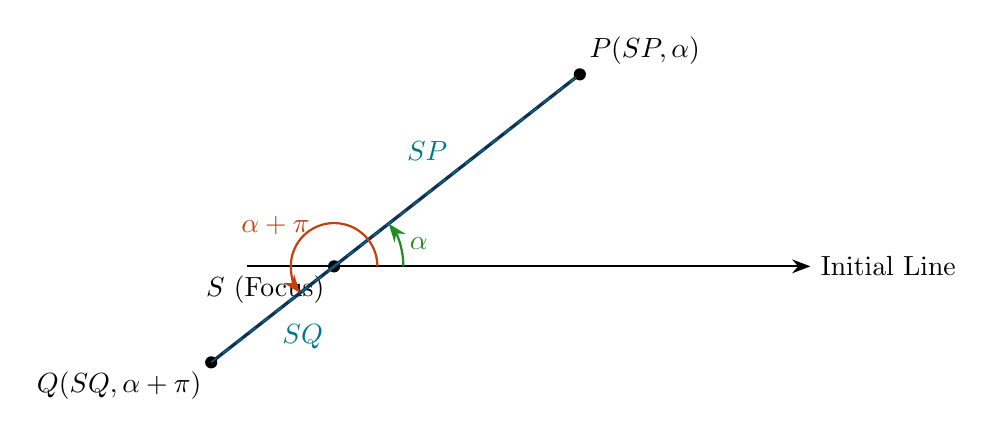
\begin{tikzpicture}[scale=1.1, >=Stealth]
    \coordinate (S) at (0,0);
    \node[below left] at (S) {$S \text{ (Focus)}$};
    \fill (S) circle (2pt);

    \draw[->, thick] (-1,0) -- (5.5,0) node[right] {Initial Line};

    % Focal Chord PSQ
    \coordinate (P) at (38:3.6);
    \coordinate (Q) at (218:1.8);
    \draw[very thick, primary] (Q) -- (P);
    \node[above right] at (P) {$P(SP, \alpha)$};
    \node[below left] at (Q) {$Q(SQ, \alpha+\pi)$};
    \fill (P) circle (2pt);
    \fill (Q) circle (2pt);

    % Segment labels
    \draw[dashed, secondary] (S) -- (P) node[midway, above left] {$SP$};
    \draw[dashed, secondary] (S) -- (Q) node[midway, below right] {$SQ$};

    % Angles
    \draw[->, thick, ForestGreen] (0.8,0) arc (0:38:0.8) node[midway, right] {$\alpha$};
    \draw[->, thick, accent] (0.5,0) arc (0:218:0.5) node[midway, left] {$\alpha+\pi$};
\end{tikzpicture}
\end{center}

\begin{theorembox}[Theorem: Harmonic Mean Property of Focal Chords]
The semi-latus rectum of any conic is the harmonic mean between the segments of any focal chord:
\begin{equation}
    \boxed{\frac{1}{SP} + \frac{1}{SQ} = \frac{2}{l} = \text{constant}}
\end{equation}
\end{theorembox}

\begin{proof}
Since $P(SP, \alpha)$ lies on the conic $\frac{l}{r} = 1 + e\cos\theta$:
\begin{equation}
    \frac{l}{SP} = 1 + e\cos\alpha. \label{eq:p2_P}
\end{equation}
Similarly, since $Q(SQ, \alpha + \pi)$ lies on the conic:
\begin{align}
    \frac{l}{SQ} &= 1 + e\cos(\alpha + \pi) \nonumber\\
                 &= 1 - e\cos\alpha. \label{eq:p2_Q}
\end{align}
Adding equations \eqref{eq:p2_P} and \eqref{eq:p2_Q} side by side:
\begin{align}
    \frac{l}{SP} + \frac{l}{SQ} &= (1 + e\cos\alpha) + (1 - e\cos\alpha) \nonumber\\
                                &= 2.
\end{align}
Dividing both sides by $l$:
\begin{equation}
    \frac{1}{SP} + \frac{1}{SQ} = \frac{2}{l}.
\end{equation}
Since $l$ is a fixed constant for a given conic, the sum of the reciprocals of the focal segments $SP$ and $SQ$ is constant and completely independent of the inclination $\alpha$ of the focal chord.
\end{proof}

\begin{notebox}[Pedagogical Significance]
This result proves that regardless of how a focal chord is rotated about the focus, the harmonic mean of its two parts $SP$ and $SQ$ remains strictly invariant and equal to the semi-latus rectum $l$.
\end{notebox}

% =========================================================================
% PAGE 03
% =========================================================================
\newpage
\section{Page 3: Equation of a Chord Joining Points $(\alpha \pm \beta)$}
\label{sec:page03}

\begin{conceptbox}[Manuscript Overview: Page 3]
Page 3 derives the general equation of a secant straight line joining two points on the conic $\frac{l}{r} = 1 + e\cos\theta$ whose vectorial angles are chosen symmetrically as $\alpha - \beta$ and $\alpha + \beta$.
\end{conceptbox}

\subsection{Algebraic Derivation}
The general equation of a straight line in polar coordinates can be written in the linear harmonic form:
\begin{equation}
    \frac{l}{r} = A\cos\theta + B\sin\theta. \label{eq:p3_genline}
\end{equation}
Equivalently, it can be re-parameterized as:
\begin{equation}
    \frac{l}{r} = e\cos\theta + C\cos(\theta - \delta).
\end{equation}
Let this straight line pass through the two points on the conic:
\begin{equation}
    P\left(r_1, \; \alpha - \beta\right) \quad \text{and} \quad Q\left(r_2, \; \alpha + \beta\right).
\end{equation}
Since $P$ lies on the conic:
\begin{equation}
    \frac{l}{r_1} = 1 + e\cos(\alpha - \beta).
\end{equation}
Since $P$ also lies on the chord \eqref{eq:p3_genline}:
\begin{equation}
    \frac{l}{r_1} = A\cos(\alpha - \beta) + B\sin(\alpha - \beta).
\end{equation}
Equating the two expressions for $\frac{l}{r_1}$:
\begin{equation}
    A\cos(\alpha - \beta) + B\sin(\alpha - \beta) = 1 + e\cos(\alpha - \beta) \iff (A - e)\cos(\alpha - \beta) + B\sin(\alpha - \beta) = 1. \label{eq:p3_eq1}
\end{equation}
Similarly, for point $Q(r_2, \alpha + \beta)$:
\begin{equation}
    (A - e)\cos(\alpha + \beta) + B\sin(\alpha + \beta) = 1. \label{eq:p3_eq2}
\end{equation}

Subtracting equation \eqref{eq:p3_eq2} from equation \eqref{eq:p3_eq1}:
\begin{align}
    (A - e)[\cos(\alpha - \beta) - \cos(\alpha + \beta)] + B[\sin(\alpha - \beta) - \sin(\alpha + \beta)] &= 0 \nonumber\\
    (A - e)[2\sin\alpha\sin\beta] - B[2\cos\alpha\sin\beta] &= 0.
\end{align}
Assuming $\beta \neq 0$ (so that $\sin\beta \neq 0$), dividing by $2\sin\beta$ yields:
\begin{equation}
    (A - e)\sin\alpha - B\cos\alpha = 0 \implies \frac{A - e}{\cos\alpha} = \frac{B}{\sin\alpha} = k.
\end{equation}
Thus:
\begin{equation}
    A - e = k\cos\alpha \implies A = e + k\cos\alpha, \quad \text{and} \quad B = k\sin\alpha.
\end{equation}
Substitute these back into equation \eqref{eq:p3_eq1}:
\begin{align}
    (k\cos\alpha)\cos(\alpha - \beta) + (k\sin\alpha)\sin(\alpha - \beta) &= 1 \nonumber\\
    k[\cos\alpha\cos(\alpha - \beta) + \sin\alpha\sin(\alpha - \beta)] &= 1 \nonumber\\
    k\cos[\alpha - (\alpha - \beta)] &= 1 \nonumber\\
    k\cos\beta &= 1 \implies k = \sec\beta.
\end{align}
Therefore:
\begin{equation}
    A = e + \sec\beta\cos\alpha, \quad B = \sec\beta\sin\alpha.
\end{equation}
Substituting $A$ and $B$ into the line equation $\frac{l}{r} = A\cos\theta + B\sin\theta$:
\begin{align}
    \frac{l}{r} &= (e + \sec\beta\cos\alpha)\cos\theta + (\sec\beta\sin\alpha)\sin\theta \nonumber\\
    &= e\cos\theta + \sec\beta(\cos\theta\cos\alpha + \sin\theta\sin\alpha) \nonumber\\
    &= e\cos\theta + \sec\beta\cos(\theta - \alpha).
\end{align}

\begin{theorembox}[Equation of a Chord in Symmetric Polar Form]
The straight line joining the points on $\frac{l}{r} = 1 + e\cos\theta$ with vectorial angles $\alpha - \beta$ and $\alpha + \beta$ is:
\begin{equation}
    \boxed{\frac{l}{r} = e\cos\theta + \sec\beta\cos(\theta - \alpha)}
\end{equation}
\end{theorembox}

% =========================================================================
% PAGE 04
% =========================================================================
\newpage
\section{Page 4: Alternate Chord Form and the Tangent at Point $\alpha$}
\label{sec:page04}

\begin{conceptbox}[Manuscript Overview: Page 4]
Page 4 rewrites the chord equation for two arbitrary vectorial angles $\alpha$ and $\beta$, derives the equation of the tangent line as the limiting case, and establishes the condition for tangency of a general line.
\end{conceptbox}

\subsection{Chord Joining Vectorial Angles $\alpha$ and $\beta$}
Let the two endpoints be given directly as $P(\alpha)$ and $Q(\beta)$.
Their mean angle is $\frac{\alpha + \beta}{2}$ and their half-difference is $\frac{\alpha - \beta}{2}$.
Setting the mean angle as $\alpha'$ and half-difference as $\beta'$ in the formula from Page 3:
\begin{equation}
    \boxed{\frac{l}{r} = e\cos\theta + \sec\left(\frac{\alpha - \beta}{2}\right)\cos\left(\theta - \frac{\alpha + \beta}{2}\right)}
\end{equation}

\subsection{Derivation of the Tangent at Point $\alpha$}
The tangent line to the conic at point $P(\alpha)$ is the limiting position of the secant chord joining $\alpha - \beta$ and $\alpha + \beta$ as the second point approaches the first, which corresponds to the limit $\beta \to 0$.
Since $\lim_{\beta \to 0} \sec\beta = \sec 0 = 1$:

\begin{theorembox}[Equation of the Tangent Line]
The equation of the tangent to the conic $\frac{l}{r} = 1 + e\cos\theta$ at the point with vectorial angle $\alpha$ is:
\begin{equation}
    \boxed{\frac{l}{r} = e\cos\theta + \cos(\theta - \alpha)}
\end{equation}
Expanding the cosine term:
\begin{equation}
    \boxed{\frac{l}{r} = (e + \cos\alpha)\cos\theta + \sin\alpha\sin\theta}
\end{equation}
\end{theorembox}

\subsection{Condition of Tangency for a Straight Line}
Let a straight line be given by:
\begin{equation}
    \frac{l}{r} = A\cos\theta + B\sin\theta. \label{eq:p4_testline}
\end{equation}
Comparing equation \eqref{eq:p4_testline} with the tangent equation $\frac{l}{r} = (e + \cos\alpha)\cos\theta + \sin\alpha\sin\theta$:
\begin{equation}
    A = e + \cos\alpha \implies A - e = \cos\alpha, \quad \text{and} \quad B = \sin\alpha.
\end{equation}
Squaring and adding:
\begin{equation}
    (A - e)^2 + B^2 = \cos^2\alpha + \sin^2\alpha = 1.
\end{equation}

\begin{theorembox}[Condition of Tangency]
The straight line $\frac{l}{r} = A\cos\theta + B\sin\theta$ touches the conic $\frac{l}{r} = 1 + e\cos\theta$ if and only if:
\begin{equation}
    \boxed{(A - e)^2 + B^2 = 1}
\end{equation}
\end{theorembox}

% =========================================================================
% PAGE 05
% =========================================================================
\newpage
\section{Page 5: Condition of Tangency and the Normal Line}
\label{sec:page05}

\begin{conceptbox}[Manuscript Overview: Page 5]
Page 5 expresses the tangency condition in perpendicular distance form $r\cos(\theta-\phi) = p$ and derives the polar equation of the normal line to the conic at point $\alpha$.
\end{conceptbox}

\subsection{Tangency Condition in Standard Form $r\cos(\theta - \phi) = p$}
Let the straight line be given in perpendicular normal form:
\begin{equation}
    r\cos(\theta - \phi) = p \iff \frac{p}{r} = \cos\theta\cos\phi + \sin\theta\sin\phi.
\end{equation}
Multiplying by $\frac{l}{p}$:
\begin{equation}
    \frac{l}{r} = \left(\frac{l}{p}\cos\phi\right)\cos\theta + \left(\frac{l}{p}\sin\phi\right)\sin\theta.
\end{equation}
Setting $A = \frac{l}{p}\cos\phi$ and $B = \frac{l}{p}\sin\phi$ into the condition $(A - e)^2 + B^2 = 1$:
\begin{align}
    \left(\frac{l}{p}\cos\phi - e\right)^2 + \left(\frac{l}{p}\sin\phi\right)^2 &= 1 \nonumber\\
    \frac{l^2}{p^2}\cos^2\phi - \frac{2le}{p}\cos\phi + e^2 + \frac{l^2}{p^2}\sin^2\phi &= 1 \nonumber\\
    \frac{l^2}{p^2}(\cos^2\phi + \sin^2\phi) - \frac{2le}{p}\cos\phi + e^2 &= 1 \nonumber\\
    \frac{l^2}{p^2} - \frac{2le}{p}\cos\phi + e^2 &= 1.
\end{align}
Multiplying through by $p^2$:
\begin{equation}
    \boxed{(l\cos\phi - ep)^2 + l^2\sin^2\phi = p^2 \iff l^2 - 2elp\cos\phi + p^2(e^2 - 1) = 0}
\end{equation}

\subsection{Derivation of the Equation of the Normal Line}
The normal line at point $P(\alpha)$ is the straight line through $P$ perpendicular to the tangent at $P$.
The equation of the tangent at $P(\alpha)$ is:
\begin{equation}
    \frac{l}{r} = (e + \cos\alpha)\cos\theta + \sin\alpha\sin\theta.
\end{equation}
In Cartesian coordinates, setting $x = r\cos\theta, y = r\sin\theta$:
\begin{equation}
    (e + \cos\alpha)x + (\sin\alpha)y = l.
\end{equation}
The slope of this tangent line is:
\begin{equation}
    m_T = -\frac{e + \cos\alpha}{\sin\alpha}.
\end{equation}
The slope of the normal line must satisfy $m_N \cdot m_T = -1$:
\begin{equation}
    m_N = \frac{\sin\alpha}{e + \cos\alpha}.
\end{equation}
The equation of any line perpendicular to the tangent is:
\begin{equation}
    -(\sin\alpha)x + (e + \cos\alpha)y = K.
\end{equation}
Converting to polar coordinates:
\begin{equation}
    r[-\sin\alpha\cos\theta + (e + \cos\alpha)\sin\theta] = K \implies r[e\sin\theta + \sin(\theta - \alpha)] = K.
\end{equation}
Since this line passes through $P(r_\alpha, \alpha)$ on the conic, where $r_\alpha = \frac{l}{1 + e\cos\alpha}$:
\begin{equation}
    K = r_\alpha [e\sin\alpha + \sin(\alpha - \alpha)] = \frac{l \cdot e\sin\alpha}{1 + e\cos\alpha}.
\end{equation}

\begin{theorembox}[Equation of the Normal Line in Polar Form]
\begin{equation}
    \boxed{\frac{le\sin\alpha}{1 + e\cos\alpha} \cdot \frac{1}{r} = e\sin\theta + \sin(\theta - \alpha)}
\end{equation}
\end{theorembox}

% =========================================================================
% PAGE 06
% =========================================================================
\newpage
\section{Page 6: Chord of Contact and the Polar Line}
\label{sec:page06}

\begin{conceptbox}[Manuscript Overview: Page 6]
Page 6 derives the equation of the chord of contact of tangents drawn from an external point $T(r_1, \theta_1)$ to the conic, and defines the polar of a point with respect to a conic.
\end{conceptbox}

\subsection{Derivation of the Chord of Contact}
Let $T(r_1, \theta_1)$ be an external point from which two tangents are drawn to the conic $\frac{l}{r} = 1 + e\cos\theta$, touching the curve at points $P(\alpha)$ and $Q(\beta)$.
The equation of the tangent at any point with vectorial angle $\phi$ is:
\begin{equation}
    \frac{l}{r} = e\cos\theta + \cos(\theta - \phi).
\end{equation}
Since both tangents pass through $T(r_1, \theta_1)$:
\begin{align}
    \frac{l}{r_1} - e\cos\theta_1 &= \cos(\theta_1 - \alpha), \label{eq:p6_tang1}\\
    \frac{l}{r_1} - e\cos\theta_1 &= \cos(\theta_1 - \beta). \label{eq:p6_tang2}
\end{align}
Now consider the equation of the chord joining $\alpha$ and $\beta$:
\begin{equation}
    \frac{l}{r} = e\cos\theta + \sec\left(\frac{\alpha - \beta}{2}\right)\cos\left(\theta - \frac{\alpha + \beta}{2}\right).
\end{equation}
From equations \eqref{eq:p6_tang1} and \eqref{eq:p6_tang2}, since $\cos(\theta_1 - \alpha) = \cos(\theta_1 - \beta)$, we have:
\begin{equation}
    \theta_1 - \alpha = -(\theta_1 - \beta) \implies \theta_1 = \frac{\alpha + \beta}{2}.
\end{equation}
Moreover:
\begin{equation}
    \frac{l}{r_1} - e\cos\theta_1 = \cos\left(\frac{\alpha - \beta}{2}\right) \implies \sec\left(\frac{\alpha - \beta}{2}\right) = \frac{1}{\frac{l}{r_1} - e\cos\theta_1}.
\end{equation}
Substituting these into the chord equation:
\begin{align}
    \frac{l}{r} - e\cos\theta &= \frac{\cos(\theta - \theta_1)}{\frac{l}{r_1} - e\cos\theta_1}.
\end{align}
Cross-multiplying yields:

\begin{theorembox}[Equation of the Chord of Contact and Polar Line]
The equation of the chord of contact of tangents from $T(r_1, \theta_1)$ (and the \textbf{polar} of $T$) with respect to $\frac{l}{r} = 1 + e\cos\theta$ is:
\begin{equation}
    \boxed{\left(\frac{l}{r} - e\cos\theta\right)\left(\frac{l}{r_1} - e\cos\theta_1\right) = \cos(\theta - \theta_1)}
\end{equation}
\end{theorembox}

% =========================================================================
% PAGE 07
% =========================================================================
\newpage
\section{Page 7: Classification of Conics and Analysis of Eccentricity}
\label{sec:page07}

\begin{conceptbox}[Manuscript Overview: Page 7]
Page 7 deals with transforming arbitrary polar equations into the standard canonical form $\frac{l'}{r} = 1 \pm e'\cos\theta$ to determine the eccentricity, semi-latus rectum, and geometric nature of the conic.
\end{conceptbox}

\subsection{Canonical Reduction Method}
Given an equation of the form:
\begin{equation}
    \frac{A}{r} = B + C\cos\theta + D\sin\theta,
\end{equation}
we reduce it to the standard canonical form:
\begin{enumerate}
    \item Divide throughout by the constant term $B$ ($B \neq 0$):
    \begin{equation}
        \frac{A/B}{r} = 1 + \frac{C}{B}\cos\theta + \frac{D}{B}\sin\theta.
    \end{equation}
    \item Combine the cosine and sine terms using $R = \sqrt{(C/B)^2 + (D/B)^2}$ and $\tan\phi = D/C$:
    \begin{equation}
        \frac{A/B}{r} = 1 + R\cos(\theta - \phi).
    \end{equation}
    \item Identify the parameters:
    \begin{equation}
        \text{Semi-latus rectum } l' = \frac{A}{B}, \quad \text{Eccentricity } e' = R = \frac{\sqrt{C^2 + D^2}}{|B|}.
    \end{equation}
\end{enumerate}

\subsection{Detailed Analysis of the Manuscript Example}
The manuscript analyzes the equation:
\begin{equation}
    \frac{l}{r} = 4 - 5\cos\theta.
\end{equation}
Dividing throughout by $4$:
\begin{equation}
    \frac{l/4}{r} = 1 - \frac{5}{4}\cos\theta.
\end{equation}
Comparing with $\frac{l'}{r} = 1 - e\cos\theta$:
\begin{itemize}[noitemsep]
    \item Semi-latus rectum: $l' = \frac{l}{4}$
    \item Eccentricity: $e = \frac{5}{4} = 1.25$
\end{itemize}

\begin{notebox}[Correction of Manuscript Slip]
In the manuscript notes on Page 7, the student wrote:
\begin{equation*}
    \text{``Since } e = \frac{5}{4} \dots \text{ ellipse''} \quad \text{\textbf{[ERROR]}}
\end{equation*}
By the fundamental definition of conic sections:
\begin{itemize}[noitemsep]
    \item If $e < 1$, the conic is an \textbf{ellipse}.
    \item If $e = 1$, the conic is a \textbf{parabola}.
    \item If $e > 1$, the conic is a \textbf{hyperbola}.
\end{itemize}
Since $e = \frac{5}{4} = 1.25 > 1$, this conic is unambiguously a \textbf{hyperbola}.
\end{notebox}

% =========================================================================
% PAGE 08
% =========================================================================
\newpage
\section{Page 8: Asymptotes of a Hyperbola in Polar Coordinates}
\label{sec:page08}

\begin{conceptbox}[Manuscript Overview: Page 8]
Page 8 derives the equations of the asymptotes of a hyperbola in polar coordinates. An asymptote is defined analytically as a tangent line whose point of contact lies at infinity.
\end{conceptbox}

\subsection{Mathematical Derivation}
Let the hyperbola have equation:
\begin{equation}
    \frac{l}{r} = 1 + e\cos\theta, \quad (e > 1).
\end{equation}
The point of contact $(\infty, \alpha)$ lies at infinity as $r \to \infty$. In this limit, $\frac{l}{r} \to 0$:
\begin{equation}
    1 + e\cos\alpha = 0 \implies \cos\alpha = -\frac{1}{e}.
\end{equation}
Since $\sin^2\alpha = 1 - \cos^2\alpha$:
\begin{equation}
    \sin\alpha = \pm \sqrt{1 - \left(-\frac{1}{e}\right)^2} = \pm \sqrt{1 - \frac{1}{e^2}} = \pm \frac{\sqrt{e^2 - 1}}{e}.
\end{equation}
The general equation of the tangent at point $\alpha$ is:
\begin{align}
    \frac{l}{r} &= e\cos\theta + \cos(\theta - \alpha) \nonumber\\
                &= e\cos\theta + \cos\theta\cos\alpha + \sin\theta\sin\alpha \nonumber\\
                &= (e + \cos\alpha)\cos\theta + (\sin\alpha)\sin\theta.
\end{align}
Substituting $\cos\alpha = -\frac{1}{e}$ and $\sin\alpha = \pm \sqrt{1 - \frac{1}{e^2}}$:
\begin{align}
    \frac{l}{r} &= \left(e - \frac{1}{e}\right)\cos\theta \pm \sqrt{1 - \frac{1}{e^2}}\sin\theta.
\end{align}
Transposing the cosine term:
\begin{equation}
    \frac{l}{r} - \left(e - \frac{1}{e}\right)\cos\theta = \pm \sqrt{1 - \frac{1}{e^2}}\sin\theta.
\end{equation}
Squaring both sides to combine both asymptotes into a single second-degree equation:

\begin{theorembox}[Combined Equation of Asymptotes]
The combined polar equation of the pair of asymptotes of the hyperbola $\frac{l}{r} = 1 + e\cos\theta$ is:
\begin{equation}
    \boxed{\left[\frac{l}{r} - \left(e - \frac{1}{e}\right)\cos\theta\right]^2 = \left(1 - \frac{1}{e^2}\right)\sin^2\theta}
\end{equation}
\end{theorembox}

% =========================================================================
% PAGE 09
% =========================================================================
\newpage
\section{Page 9: Problem 1 --- Tangent Segment Intercepted by Directrix}
\label{sec:page09}

\begin{examplebox}[Problem 1 (Manuscript Page 9)]
\textbf{Problem Statement:}
Prove that the portion of any tangent to a conic intercepted between the curve and the directrix subtends a right angle at the corresponding focus.
\tcblower
\textbf{Proof:}
Let the focus $S$ be taken as the pole, and let the conic be:
\begin{equation}
    \frac{l}{r} = 1 + e\cos\theta.
\end{equation}
The directrix corresponding to the focus $S$ is the line $r\cos\theta = -\frac{l}{e} \iff \frac{l}{r} = -e\cos\theta$.
Let $P(\alpha)$ be any point of contact on the conic. The equation of the tangent at $P$ is:
\begin{equation}
    \frac{l}{r} = e\cos\theta + \cos(\theta - \alpha). \label{eq:p9_tan}
\end{equation}
Let this tangent intersect the directrix at point $K(r_K, \theta_K)$.
At the directrix, $\frac{l}{r_K} = -e\cos\theta_K$.
Substituting this into equation \eqref{eq:p9_tan}:
\begin{align}
    -e\cos\theta_K &= e\cos\theta_K + \cos(\theta_K - \alpha) \nonumber\\
    \cos(\theta_K - \alpha) &= -2e\cos\theta_K.
\end{align}
If we use the standard directrix $\frac{l}{r} = e\cos\theta$:
\begin{align}
    e\cos\theta_K &= e\cos\theta_K + \cos(\theta_K - \alpha) \nonumber\\
    \cos(\theta_K - \alpha) &= 0.
\end{align}
Hence:
\begin{equation}
    \theta_K - \alpha = \pm \frac{\pi}{2} \iff |\angle KSP| = \frac{\pi}{2} = 90^\circ.
\end{equation}
Thus, the intercepted segment $PK$ subtends a right angle ($90^\circ$) at the focus $S$.
\end{examplebox}

% =========================================================================
% PAGE 10
% =========================================================================
\newpage
\section{Page 10: Problem 2 --- Sum of Reciprocal Products of Focal Chords}
\label{sec:page10}

\begin{examplebox}[Problem 2 (Manuscript Page 10)]
\textbf{Problem Statement:}
If $PSP'$ and $QSQ'$ are two mutually perpendicular focal chords of a conic $\frac{l}{r} = 1 + e\cos\theta$, prove that:
\begin{equation*}
    \frac{1}{SP \cdot SP'} + \frac{1}{SQ \cdot SQ'} = \text{constant}.
\end{equation*}
\tcblower
\textbf{Solution:}
Let the vectorial angle of $P$ be $\alpha$. Since $PSP'$ is a straight line through the pole $S$, the vectorial angle of $P'$ is $\alpha + \pi$.
From the equation of the conic:
\begin{align}
    \frac{l}{SP} &= 1 + e\cos\alpha, \\
    \frac{l}{SP'} &= 1 + e\cos(\alpha + \pi) = 1 - e\cos\alpha.
\end{align}
Multiplying these two relations:
\begin{align}
    \frac{l^2}{SP \cdot SP'} &= (1 + e\cos\alpha)(1 - e\cos\alpha) = 1 - e^2\cos^2\alpha \nonumber\\
    \frac{1}{SP \cdot SP'} &= \frac{1 - e^2\cos^2\alpha}{l^2}. \label{eq:p10_1}
\end{align}
Since $QSQ'$ is perpendicular to $PSP'$, the vectorial angle of $Q$ is $\alpha + \frac{\pi}{2}$, and that of $Q'$ is $\alpha + \frac{3\pi}{2}$.
Hence:
\begin{align}
    \frac{l}{SQ} &= 1 + e\cos\left(\alpha + \frac{\pi}{2}\right) = 1 - e\sin\alpha, \\
    \frac{l}{SQ'} &= 1 + e\cos\left(\alpha + \frac{3\pi}{2}\right) = 1 + e\sin\alpha.
\end{align}
Multiplying:
\begin{align}
    \frac{l^2}{SQ \cdot SQ'} &= (1 - e\sin\alpha)(1 + e\sin\alpha) = 1 - e^2\sin^2\alpha \nonumber\\
    \frac{1}{SQ \cdot SQ'} &= \frac{1 - e^2\sin^2\alpha}{l^2}. \label{eq:p10_2}
\end{align}
Adding equations \eqref{eq:p10_1} and \eqref{eq:p10_2}:
\begin{align}
    \frac{1}{SP \cdot SP'} + \frac{1}{SQ \cdot SQ'} &= \frac{(1 - e^2\cos^2\alpha) + (1 - e^2\sin^2\alpha)}{l^2} \nonumber\\
    &= \frac{2 - e^2(\cos^2\alpha + \sin^2\alpha)}{l^2} \nonumber\\
    &= \boxed{\frac{2 - e^2}{l^2} = \text{constant}}
\end{align}
This quantity is completely independent of $\alpha$, completing the proof.
\end{examplebox}

% =========================================================================
% PAGE 11
% =========================================================================
\newpage
\section{Page 11: Problem 3 --- Tangents at Extremities of a Focal Chord}
\label{sec:page11}

\begin{examplebox}[Problem 3 (Manuscript Page 11)]
\textbf{Problem Statement:}
Prove that the tangents at the ends of any focal chord of a conic intersect on the corresponding directrix.
\tcblower
\textbf{Proof:}
Let $PSQ$ be any focal chord of the conic $\frac{l}{r} = 1 + e\cos\theta$.
Let the vectorial angle of $P$ be $\alpha$. Then the vectorial angle of $Q$ is $\alpha + \pi$.
The equation of the tangent at $P(\alpha)$ is:
\begin{equation}
    \frac{l}{r} = e\cos\theta + \cos(\theta - \alpha). \label{eq:p11_tan1}
\end{equation}
The equation of the tangent at $Q(\alpha + \pi)$ is:
\begin{align}
    \frac{l}{r} &= e\cos\theta + \cos[\theta - (\alpha + \pi)] \nonumber\\
                &= e\cos\theta + \cos[(\theta - \alpha) - \pi] \nonumber\\
                &= e\cos\theta - \cos(\theta - \alpha). \label{eq:p11_tan2}
\end{align}
To find their point of intersection, subtract equation \eqref{eq:p11_tan2} from equation \eqref{eq:p11_tan1}:
\begin{equation}
    2\cos(\theta - \alpha) = 0 \implies \cos(\theta - \alpha) = 0.
\end{equation}
Substituting $\cos(\theta - \alpha) = 0$ back into equation \eqref{eq:p11_tan1}:
\begin{equation}
    \frac{l}{r} = e\cos\theta.
\end{equation}
This is precisely the equation of the directrix of the conic.
Hence, the point of intersection of the tangents at the extremities of any focal chord always lies on the directrix.
\end{examplebox}

% =========================================================================
% PAGE 12
% =========================================================================
\newpage
\section{Page 12: Problem 4 --- Perpendicular Focal Tangents of a Parabola}
\label{sec:page12}

\begin{examplebox}[Problem 4 (Manuscript Page 12)]
\textbf{Problem Statement:}
For a parabola ($e = 1$), prove that the tangents at the ends of any focal chord intersect at right angles on the directrix.
\tcblower
\textbf{Proof:}
For a parabola, $e = 1$, and its equation is:
\begin{equation}
    \frac{l}{r} = 1 + \cos\theta.
\end{equation}
Let $PSQ$ be a focal chord with $P$ at $\alpha$ and $Q$ at $\alpha + \pi$.
From Page 11, the tangents intersect on the directrix where $\cos(\theta - \alpha) = 0 \implies \theta = \alpha \pm \frac{\pi}{2}$.
Now consider the inclination of the tangents.
In Cartesian coordinates, the equation of the tangent at point $\alpha$ is:
\begin{equation}
    (1 + \cos\alpha)x + (\sin\alpha)y = l \implies 2\cos^2\left(\frac{\alpha}{2}\right)x + 2\sin\left(\frac{\alpha}{2}\right)\cos\left(\frac{\alpha}{2}\right)y = l.
\end{equation}
The slope of this tangent is:
\begin{equation}
    m_1 = -\frac{1 + \cos\alpha}{\sin\alpha} = -\frac{2\cos^2(\alpha/2)}{2\sin(\alpha/2)\cos(\alpha/2)} = -\cot\left(\frac{\alpha}{2}\right).
\end{equation}
Similarly, the slope of the tangent at $Q(\alpha + \pi)$ is obtained by replacing $\alpha$ with $\alpha + \pi$:
\begin{align}
    m_2 &= -\cot\left(\frac{\alpha + \pi}{2}\right) = -\cot\left(\frac{\alpha}{2} + \frac{\pi}{2}\right) = - \left(-\tan\frac{\alpha}{2}\right) = \tan\left(\frac{\alpha}{2}\right).
\end{align}
Evaluating the product of the slopes:
\begin{equation}
    m_1 \cdot m_2 = \left[-\cot\left(\frac{\alpha}{2}\right)\right] \cdot \left[\tan\left(\frac{\alpha}{2}\right)\right] = -1.
\end{equation}
Since $m_1 m_2 = -1$, the two tangents are mutually perpendicular ($90^\circ$).
Thus, for a parabola, the tangents at the ends of any focal chord intersect at right angles on the directrix.
\end{examplebox}

% =========================================================================
% PAGE 13
% =========================================================================
\newpage
\section{Page 13: Problem 5 --- Director Circle in Polar Coordinates}
\label{sec:page13}

\begin{examplebox}[Problem 5 (Manuscript Page 13)]
\textbf{Problem Statement:}
Find the locus of the point of intersection of two perpendicular tangents to the conic $\frac{l}{r} = 1 + e\cos\theta$ (Equation of the Director Circle).
\tcblower
\textbf{Solution:}
Let the tangents be drawn at points with vectorial angles $\alpha$ and $\beta$.
Their equations are:
\begin{align}
    \frac{l}{r} &= (e + \cos\alpha)\cos\theta + \sin\alpha\sin\theta, \\
    \frac{l}{r} &= (e + \cos\beta)\cos\theta + \sin\beta\sin\theta.
\end{align}
Their Cartesian slopes are:
\begin{equation}
    m_1 = -\frac{e + \cos\alpha}{\sin\alpha}, \quad m_2 = -\frac{e + \cos\beta}{\sin\beta}.
\end{equation}
Since the tangents are perpendicular, $m_1 m_2 = -1$:
\begin{align}
    \frac{(e + \cos\alpha)(e + \cos\beta)}{\sin\alpha\sin\beta} &= -1 \nonumber\\
    e^2 + e(\cos\alpha + \cos\beta) + \cos\alpha\cos\beta + \sin\alpha\sin\beta &= 0 \nonumber\\
    e^2 + 2e\cos\left(\frac{\alpha+\beta}{2}\right)\cos\left(\frac{\alpha-\beta}{2}\right) + \cos(\alpha - \beta) &= 0. \label{eq:p13_perp}
\end{align}
Let $(r_0, \theta_0)$ be the coordinates of their point of intersection.
Solving the two tangent equations simultaneously gives:
\begin{equation}
    \theta_0 = \frac{\alpha + \beta}{2}, \quad \text{and} \quad \frac{l}{r_0} = e\cos\theta_0 + \cos\left(\frac{\alpha - \beta}{2}\right).
\end{equation}
Let $\gamma = \frac{\alpha - \beta}{2}$. Then $\cos\gamma = \frac{l}{r_0} - e\cos\theta_0$, and $\cos(\alpha - \beta) = 2\cos^2\gamma - 1$.
Substituting into equation \eqref{eq:p13_perp}:
\begin{align}
    e^2 + 2e\cos\theta_0\left(\frac{l}{r_0} - e\cos\theta_0\right) + 2\left(\frac{l}{r_0} - e\cos\theta_0\right)^2 - 1 &= 0 \nonumber\\
    e^2 - 1 + \frac{2el}{r_0}\cos\theta_0 - 2e^2\cos^2\theta_0 + 2\left(\frac{l^2}{r_0^2} - \frac{2el}{r_0}\cos\theta_0 + e^2\cos^2\theta_0\right) &= 0 \nonumber\\
    (e^2 - 1) - \frac{2el}{r_0}\cos\theta_0 + \frac{2l^2}{r_0^2} &= 0.
\end{align}
Multiplying by $r_0^2$ and generalizing $(r_0, \theta_0) \to (r, \theta)$:
\begin{equation}
    \boxed{(e^2 - 1)r^2 - 2elr\cos\theta + 2l^2 = 0}
\end{equation}
This is the polar equation of the \textbf{director circle} of the conic.
\end{examplebox}

% =========================================================================
% PAGE 14
% =========================================================================
\newpage
\section{Page 14: Problem 6 --- Locus of the Pole of a Subtended Chord}
\label{sec:page14}

\begin{examplebox}[Problem 6 (Manuscript Page 14)]
\textbf{Problem Statement:}
Find the locus of the pole of a chord of the conic $\frac{l}{r} = 1 + e\cos\theta$ which subtends a constant angle $2\beta$ at the focus.
\tcblower
\textbf{Solution:}
Let $T(r_1, \theta_1)$ be the pole of the chord.
The chord is the chord of contact of tangents drawn from $T(r_1, \theta_1)$ to the conic.
Let the points of contact of these tangents be $P$ and $Q$, with vectorial angles $\alpha - \beta$ and $\alpha + \beta$, so that the angle subtended by the chord $PQ$ at the focus $S$ is:
\begin{equation}
    \angle PSQ = (\alpha + \beta) - (\alpha - \beta) = 2\beta = \text{constant}.
\end{equation}
The equation of the chord of contact from $T(r_1, \theta_1)$ is:
\begin{equation}
    \frac{l}{r} = e\cos\theta + \sec\beta\cos(\theta - \alpha).
\end{equation}
As derived on Page 6, the coordinates of the pole $T(r_1, \theta_1)$ satisfy:
\begin{equation}
    \theta_1 = \alpha, \quad \text{and} \quad \frac{l}{r_1} - e\cos\theta_1 = \cos\beta.
\end{equation}
Therefore:
\begin{equation}
    \frac{l}{r_1} = e\cos\theta_1 + \cos\beta.
\end{equation}
Dividing by $\cos\beta$:
\begin{equation}
    \frac{l\sec\beta}{r_1} = 1 + e\sec\beta\cos\theta_1.
\end{equation}
Generalizing to arbitrary polar coordinates $(r, \theta)$:
\begin{equation}
    \boxed{\frac{l\sec\beta}{r} = 1 + (e\sec\beta)\cos\theta}
\end{equation}
\textbf{Conclusion:}
The locus of the pole is another conic of the same type, having the same focus and axis, with new semi-latus rectum $l' = l\sec\beta$ and new eccentricity $e' = e\sec\beta$.
\end{examplebox}

\chapter{3D Cartesian Coordinates and Direction Cosines (Pages 15--24)}
\label{ch:coordinates_dc_dr}

% =========================================================================
% PAGE 15
% =========================================================================
\section{Page 15: Introduction to 3D Cartesian Coordinates and Section Formulae}
\label{sec:page15}

\begin{conceptbox}[Manuscript Overview: Page 15]
Page 15 transitions the course from two-dimensional polar geometry to three-dimensional analytical geometry. It introduces the rectangular Cartesian coordinate frame in $\mathbb{R}^3$, the definition of points $P(x_1, y_1, z_1)$ and $Q(x_2, y_2, z_2)$, the section formula dividing a segment in the ratio $m_1 : m_2$, the midpoint formula, and the concept of changing coordinates via translation of axes.
\end{conceptbox}

\subsection{The Spatial Cartesian Coordinate System}
To represent spatial configurations analytically, three mutually perpendicular straight lines are chosen that intersect at a single point $O$, known as the \textbf{origin}:
\begin{itemize}[noitemsep]
    \item $X'OX$: The \textbf{$x$-axis} (abscissa axis).
    \item $Y'OY$: The \textbf{$y$-axis}.
    \item $Z'OZ$: The \textbf{$z$-axis} (applicate axis).
\end{itemize}
These three lines define three mutually perpendicular planes, known as the \textbf{coordinate planes}:
\begin{enumerate}[noitemsep]
    \item The \textbf{$xy$-plane}: $z = 0$, spanned by the $x$- and $y$-axes.
    \item The \textbf{$yz$-plane}: $x = 0$, spanned by the $y$- and $z$-axes.
    \item The \textbf{$zx$-plane}: $y = 0$, spanned by the $z$- and $x$-axes.
\end{enumerate}
These planes divide the whole of three-dimensional Euclidean space into $8$ compartments, termed \textbf{octants}. The signs of the triad of real numbers $(x, y, z)$ determine the octant in which any point $P$ resides.

\begin{center}
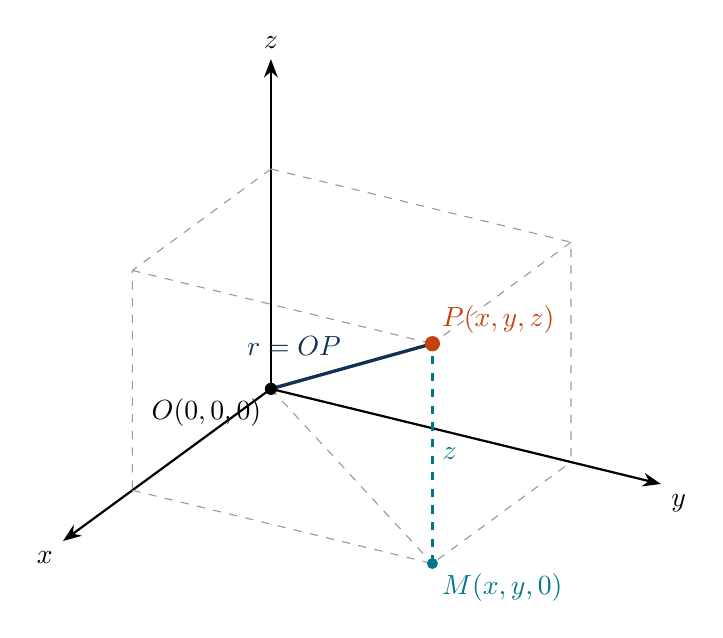
\begin{tikzpicture}[scale=1.1, >=Stealth, 3d view={120}{25}]
    % Axes
    \draw[->, thick] (0,0,0) -- (4.8,0,0) node[anchor=north east]{$x$};
    \draw[->, thick] (0,0,0) -- (0,5.2,0) node[anchor=north west]{$y$};
    \draw[->, thick] (0,0,0) -- (0,0,4.2) node[anchor=south]{$z$};

    % Origin
    \coordinate (O) at (0,0,0);
    \node[below left] at (O) {$O(0,0,0)$};

    % Coordinates of P
    \def\px{3.2}
    \def\py{4.0}
    \def\pz{2.8}

    \coordinate (P) at (\px,\py,\pz);
    \coordinate (A) at (\px,0,0);
    \coordinate (B) at (0,\py,0);
    \coordinate (C) at (0,0,\pz);
    \coordinate (M) at (\px,\py,0); % xy projection
    \coordinate (N) at (0,\py,\pz); % yz projection
    \coordinate (L) at (\px,0,\pz); % zx projection

    % Box edges
    \draw[dashed, gray!80] (A) -- (M) -- (B);
    \draw[dashed, gray!80] (O) -- (M);
    \draw[dashed, secondary, thick] (M) -- (P) node[midway, right] {$z$};
    \draw[dashed, gray!80] (C) -- (L) -- (A);
    \draw[dashed, gray!80] (C) -- (N) -- (B);
    \draw[dashed, gray!80] (L) -- (P);
    \draw[dashed, gray!80] (N) -- (P);

    % Distance OP
    \draw[very thick, primary] (O) -- (P) node[midway, above left] {$r = OP$};

    % Points
    \fill (O) circle (2pt);
    \fill[accent] (P) circle (2.5pt) node[above right] {$P(x,y,z)$};
    \fill[secondary] (M) circle (1.8pt) node[below right] {$M(x,y,0)$};
\end{tikzpicture}
\end{center}

\subsection{The 3D Distance Formula}
Let $P(x_1, y_1, z_1)$ and $Q(x_2, y_2, z_2)$ be two arbitrary points in space. Construct a rectangular cuboid whose opposite vertices are $P$ and $Q$, with faces parallel to the coordinate planes. The lengths of the edges of this cuboid are:
\begin{equation}
    \Delta x = |x_2 - x_1|, \quad \Delta y = |y_2 - y_1|, \quad \Delta z = |z_2 - z_1|.
\end{equation}
By double application of the Pythagorean theorem:
\begin{equation}
    PQ^2 = (\Delta x)^2 + (\Delta y)^2 + (\Delta z)^2 = (x_2 - x_1)^2 + (y_2 - y_1)^2 + (z_2 - z_1)^2.
\end{equation}
Thus, the Euclidean distance between $P$ and $Q$ is:
\begin{equation}
    \boxed{PQ = \sqrt{(x_2 - x_1)^2 + (y_2 - y_1)^2 + (z_2 - z_1)^2}}
\end{equation}
In particular, the distance of any point $P(x, y, z)$ from the origin $O(0,0,0)$ is:
\begin{equation}
    OP = \sqrt{x^2 + y^2 + z^2}.
\end{equation}

\subsection{Section Formula (Internal and External Division)}
\begin{theorembox}[Section Formula in Three Dimensions]
Let $P(x_1, y_1, z_1)$ and $Q(x_2, y_2, z_2)$ be two given points. Let $R(x, y, z)$ be a point dividing the directed line segment $PQ$ in the given ratio $m_1 : m_2$.
\begin{enumerate}
    \item \textbf{Internal Division}: If $R$ lies between $P$ and $Q$,
    \begin{equation}
        \boxed{x = \frac{m_1 x_2 + m_2 x_1}{m_1 + m_2}, \quad y = \frac{m_1 y_2 + m_2 y_1}{m_1 + m_2}, \quad z = \frac{m_1 z_2 + m_2 z_1}{m_1 + m_2}}
    \end{equation}
    \item \textbf{External Division}: If $R$ lies on the line produced outside the segment $PQ$,
    \begin{equation}
        \boxed{x = \frac{m_1 x_2 - m_2 x_1}{m_1 - m_2}, \quad y = \frac{m_1 y_2 - m_2 y_1}{m_1 - m_2}, \quad z = \frac{m_1 z_2 - m_2 z_1}{m_1 - m_2}} \quad (m_1 \neq m_2).
    \end{equation}
\end{enumerate}
\end{theorembox}

\begin{proof}
Draw perpendiculars $PP', QQ', RR'$ from $P, Q, R$ respectively to the $xy$-plane. The feet of these perpendiculars $P', Q', R'$ lie in the $xy$-plane and have coordinates $(x_1, y_1, 0)$, $(x_2, y_2, 0)$, and $(x, y, 0)$.
Since $PP', RR', QQ'$ are all perpendicular to the $xy$-plane, they are parallel to one another and lie in a common plane.
Through $R$, draw a line parallel to $P'Q'$ meeting $PP'$ at $S$ and $QQ'$ at $T$.
From the elementary geometry of similar triangles $\triangle PSR \sim \triangle RTQ$:
\begin{equation}
    \frac{PR}{RQ} = \frac{m_1}{m_2} = \frac{z - z_1}{z_2 - z}.
\end{equation}
Cross-multiplying gives:
\begin{equation}
    m_1(z_2 - z) = m_2(z - z_1) \implies (m_1 + m_2)z = m_1 z_2 + m_2 z_1 \implies z = \frac{m_1 z_2 + m_2 z_1}{m_1 + m_2}.
\end{equation}
By projecting onto the $yz$-plane and $zx$-plane in an identical manner, we obtain:
\begin{equation}
    x = \frac{m_1 x_2 + m_2 x_1}{m_1 + m_2}, \quad y = \frac{m_1 y_2 + m_2 y_1}{m_1 + m_2}.
\end{equation}
For external division, replacing $m_2$ by $-m_2$ yields the required result.
\end{proof}

\begin{notebox}[Important Corollaries of the Section Formula]
\begin{itemize}[noitemsep]
    \item \textbf{Midpoint Formula}: When $m_1 : m_2 = 1 : 1$, the midpoint $M$ of segment $PQ$ is:
    \begin{equation}
        M = \left(\frac{x_1 + x_2}{2}, \; \frac{y_1 + y_2}{2}, \; \frac{z_1 + z_2}{2}\right).
    \end{equation}
    \item \textbf{Centroid of a Triangle}: If vertices are $A(x_1, y_1, z_1), B(x_2, y_2, z_2), C(x_3, y_3, z_3)$, the medians intersect at centroid $G$:
    \begin{equation}
        G = \left(\frac{x_1+x_2+x_3}{3}, \; \frac{y_1+y_2+y_3}{3}, \; \frac{z_1+z_2+z_3}{3}\right).
    \end{equation}
    \item \textbf{Centroid of a Tetrahedron}: If vertices are $A_i(x_i, y_i, z_i)$ for $i=1,2,3,4$, the centroid is:
    \begin{equation}
        G = \left(\frac{\sum x_i}{4}, \; \frac{\sum y_i}{4}, \; \frac{\sum z_i}{4}\right).
    \end{equation}
\end{itemize}
\end{notebox}

% =========================================================================
% PAGE 16
% =========================================================================
\section{Page 16: Transformation of Coordinates --- Translation of Axes}
\label{sec:page16}

\begin{conceptbox}[Manuscript Overview: Page 16]
Page 16 explores the kinematics of coordinate frames in space. It focuses on the translation of axes: shifting the origin from $O(0,0,0)$ to a new point $O'(h, k, l)$ while maintaining the parallel orientation of all three coordinate axes.
\end{conceptbox}

\subsection{Transformation Equations for Translation}
Let $OX, OY, OZ$ be the original coordinate axes with origin $O(0,0,0)$.
Let the origin be shifted to a new point $O'$ whose coordinates with respect to the original system are $(h, k, l)$.
Let through $O'$ three new axes $O'X', O'Y', O'Z'$ be drawn parallel respectively to $OX, OY, OZ$ and directed in the same sense.

\begin{center}
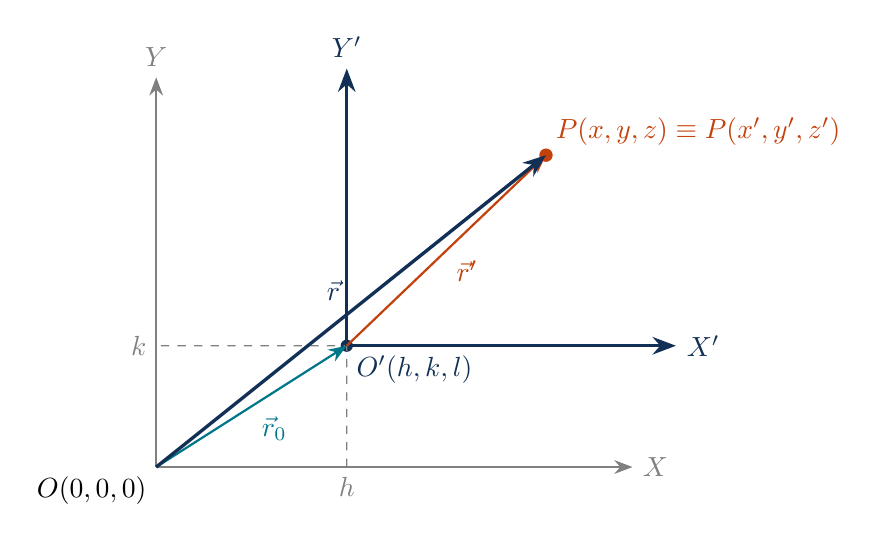
\begin{tikzpicture}[scale=1.1, >=Stealth]
    % Old axes
    \draw[->, thick, gray] (0,0) -- (5.5,0) node[right] {$X$};
    \draw[->, thick, gray] (0,0) -- (0,4.5) node[above] {$Y$};
    \node[below left] at (0,0) {$O(0,0,0)$};

    % New origin O'
    \coordinate (Oprime) at (2.2, 1.4);
    \fill[primary] (Oprime) circle (2pt) node[below right] {$O'(h,k,l)$};
    \draw[dashed, gray] (2.2,0) node[below] {$h$} -- (Oprime) -- (0,1.4) node[left] {$k$};

    % New axes
    \draw[->, very thick, primary] (Oprime) -- ++(3.8,0) node[right] {$X'$};
    \draw[->, very thick, primary] (Oprime) -- ++(0,3.2) node[above] {$Y'$};

    % Point P
    \coordinate (P) at (4.5, 3.6);
    \fill[accent] (P) circle (2.2pt) node[above right] {$P(x,y,z) \equiv P(x',y',z')$};

    % Vector arrows
    \draw[->, thick, secondary] (0,0) -- (Oprime) node[midway, below right] {$\vec{r}_0$};
    \draw[->, thick, accent] (Oprime) -- (P) node[midway, below right] {$\vec{r}'$};
    \draw[->, very thick, primary] (0,0) -- (P) node[midway, above left] {$\vec{r}$};
\end{tikzpicture}
\end{center}

Let $P$ be any point in space whose coordinates are:
\begin{itemize}[noitemsep]
    \item $(x, y, z)$ with respect to the old axes $OX, OY, OZ$.
    \item $(x', y', z')$ with respect to the new axes $O'X', O'Y', O'Z'$.
\end{itemize}

\begin{theorembox}[Transformation of Coordinates under Translation]
The relations connecting the old coordinates $(x,y,z)$ and the new coordinates $(x',y',z')$ are:
\begin{equation}
    \boxed{x = x' + h, \quad y = y' + k, \quad z = z' + l}
\end{equation}
Conversely, the new coordinates in terms of the old coordinates are:
\begin{equation}
    \boxed{x' = x - h, \quad y' = y - k, \quad z' = z - l}
\end{equation}
\end{theorembox}

\begin{proof}
Let the position vectors of $O'$ and $P$ with respect to the original origin $O$ be $\vec{r}_0$ and $\vec{r}$ respectively:
\begin{align}
    \vec{r}_0 &= h\,\hat{i} + k\,\hat{j} + l\,\hat{k}, \\
    \vec{r} &= x\,\hat{i} + y\,\hat{j} + z\,\hat{k}.
\end{align}
The position vector of $P$ relative to the new origin $O'$ is $\vec{r}' = x'\,\hat{i} + y'\,\hat{j} + z'\,\hat{k}$.
By vector addition in triangle $\triangle OO'P$:
\begin{equation}
    \vec{OP} = \vec{OO'} + \vec{O'P} \implies \vec{r} = \vec{r}_0 + \vec{r}'.
\end{equation}
Equating components along the three mutually orthogonal basis vectors $\hat{i}, \hat{j}, \hat{k}$:
\begin{equation}
    x = x' + h, \quad y = y' + k, \quad z = z' + l.
\end{equation}
\end{proof}

\subsection{Invariance of Spatial Distances}
A fundamental geometric invariant under pure translation is the Euclidean distance between any pair of points:
\begin{align}
    d^2 &= (x_2 - x_1)^2 + (y_2 - y_1)^2 + (z_2 - z_1)^2 \nonumber\\
    &= \bigl[(x'_2 + h) - (x'_1 + h)\bigr]^2 + \bigl[(y'_2 + k) - (y'_1 + k)\bigr]^2 + \bigl[(z'_2 + l) - (z'_1 + l)\bigr]^2 \nonumber\\
    &= (x'_2 - x'_1)^2 + (y'_2 - y'_1)^2 + (z'_2 - z'_1)^2.
\end{align}
Thus, distance is strictly invariant under translation of axes.

% =========================================================================
% PAGE 17
% =========================================================================
\section{Page 17: Projection of a Directed Line Segment on Coordinate Axes}
\label{sec:page17}

\begin{conceptbox}[Manuscript Overview: Page 17]
Page 17 analyzes the projection of a directed line segment $OP$ on the three rectangular coordinate axes. It establishes that the coordinates $(x,y,z)$ of any point $P$ are precisely the orthogonal projections of the position vector $\vec{OP}$ on the $x$-, $y$-, and $z$-axes.
\end{conceptbox}

\subsection{Geometric Definition of Orthogonal Projection}
The \textbf{orthogonal projection} of a directed line segment $AB$ onto a directed line $L$ is the directed segment $A'B'$ on $L$, where $A'$ and $B'$ are the feet of the perpendiculars dropped from $A$ and $B$ respectively onto $L$.
If $\theta$ is the angle between the directed segment $\vec{AB}$ and the directed line $L$, then the algebraic magnitude of the projection is:
\begin{equation}
    \text{Proj}_L(\vec{AB}) = |\vec{AB}|\cos\theta.
\end{equation}

\subsection{Projections of the Radius Vector $OP$}
Let $P(x,y,z)$ be any point in space, and let $OP = r = \sqrt{x^2+y^2+z^2}$.
Let the directed line segment $OP$ make angles $\alpha, \beta, \gamma$ with the positive directions of the coordinate axes $OX, OY, OZ$ respectively. These angles are called the \textbf{direction angles} of the line $OP$.

\begin{center}
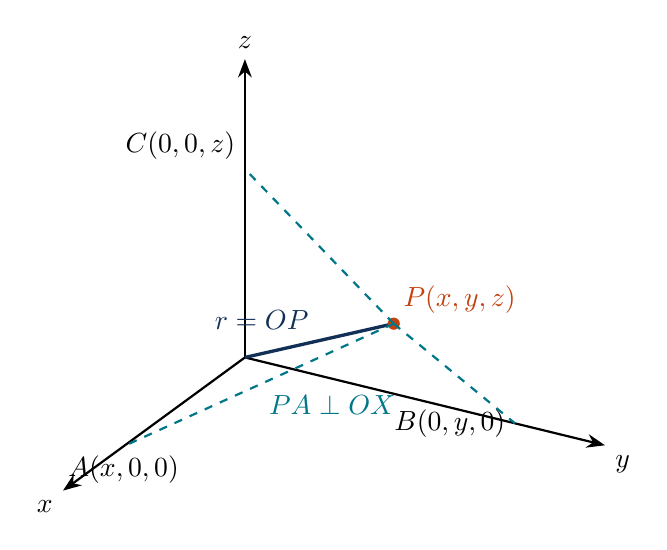
\begin{tikzpicture}[scale=1.1, >=Stealth, 3d view={120}{25}]
    % Axes
    \draw[->, thick] (0,0,0) -- (4.2,0,0) node[anchor=north east]{$x$};
    \draw[->, thick] (0,0,0) -- (0,4.8,0) node[anchor=north west]{$y$};
    \draw[->, thick] (0,0,0) -- (0,0,3.8) node[anchor=south]{$z$};

    \coordinate (O) at (0,0,0);
    \coordinate (P) at (2.8, 3.6, 2.4);
    \coordinate (A) at (2.8,0,0);
    \coordinate (B) at (0,3.6,0);
    \coordinate (C) at (0,0,2.4);

    % Segment OP
    \draw[very thick, primary] (O) -- (P) node[midway, above left] {$r = OP$};
    \fill[accent] (P) circle (2pt) node[above right] {$P(x,y,z)$};

    % Projection right triangles
    \draw[dashed, secondary, thick] (P) -- (A) node[midway, below right] {$PA \perp OX$};
    \draw[dashed, secondary, thick] (P) -- (B);
    \draw[dashed, secondary, thick] (P) -- (C);

    \node[below] at (A) {$A(x,0,0)$};
    \node[left] at (B) {$B(0,y,0)$};
    \node[above left] at (C) {$C(0,0,z)$};
\end{tikzpicture}
\end{center}

In the right-angled triangle $\triangle OAP$, the angle at $A$ is $90^\circ$ because $PA$ lies in the plane perpendicular to the $x$-axis:
\begin{equation}
    \cos\alpha = \frac{OA}{OP} = \frac{x}{r} \implies \boxed{x = r\cos\alpha}
\end{equation}
Similarly, from the right-angled triangles $\triangle OBP$ and $\triangle OCP$:
\begin{align}
    \cos\beta &= \frac{OB}{OP} = \frac{y}{r} \implies \boxed{y = r\cos\beta} \\
    \cos\gamma &= \frac{OC}{OP} = \frac{z}{r} \implies \boxed{z = r\cos\gamma}
\end{align}

\begin{theorembox}[Coordinates as Projections]
The coordinates $(x,y,z)$ of any point $P$ at distance $r$ from the origin are the orthogonal projections of the radius vector $OP$ on the three coordinate axes:
\begin{equation}
    x = r\cos\alpha, \quad y = r\cos\beta, \quad z = r\cos\gamma
\end{equation}
where $\alpha, \beta, \gamma$ are the direction angles of $OP$.
\end{theorembox}

% =========================================================================
% PAGE 18
% =========================================================================
\section{Page 18: Projection of a Broken Line --- The Contour Theorem}
\label{sec:page18}

\begin{conceptbox}[Manuscript Overview: Page 18]
Page 18 derives the fundamental projection theorem for broken polygonal lines (the \textbf{Contour Theorem}). It proves that the projection of the straight segment joining the initial point to the terminal point equals the algebraic sum of the projections of the individual segments composing the path.
\end{conceptbox}

\subsection{The Fundamental Projection Theorem}
\begin{theorembox}[Projection of a Broken Line (Contour Theorem)]
Let $P_0, P_1, P_2, \dots, P_n$ be any sequence of points in space forming a broken line (polygonal path). Then the orthogonal projection of the direct segment $P_0 P_n$ on any directed line $L$ is equal to the algebraic sum of the projections of the individual directed segments $P_0 P_1, P_1 P_2, \dots, P_{n-1} P_n$ on $L$:
\begin{equation}
    \boxed{\text{Proj}_L(P_0 P_n) = \sum_{i=1}^n \text{Proj}_L(P_{i-1} P_i)}
\end{equation}
\end{theorembox}

\begin{proof}
Let $L$ be a directed line, and let $\hat{u}$ be a unit vector along $L$.
By vector addition, the displacement vector from $P_0$ to $P_n$ is:
\begin{equation}
    \vec{P_0 P_n} = \vec{P_0 P_1} + \vec{P_1 P_2} + \vec{P_2 P_3} + \dots + \vec{P_{n-1} P_n}.
\end{equation}
The orthogonal projection of any directed segment $\vec{AB}$ on $L$ is given by the scalar dot product with the unit vector $\hat{u}$:
\begin{equation}
    \text{Proj}_L(\vec{AB}) = \vec{AB} \cdot \hat{u}.
\end{equation}
Taking the dot product of both sides with $\hat{u}$:
\begin{align}
    \vec{P_0 P_n} \cdot \hat{u} &= \left( \sum_{i=1}^n \vec{P_{i-1} P_i} \right) \cdot \hat{u} \nonumber\\
    &= \sum_{i=1}^n (\vec{P_{i-1} P_i} \cdot \hat{u}).
\end{align}
Since $\vec{P_0 P_n} \cdot \hat{u} = \text{Proj}_L(P_0 P_n)$ and $\vec{P_{i-1} P_i} \cdot \hat{u} = \text{Proj}_L(P_{i-1} P_i)$, the theorem is proved.
\end{proof}

\subsection{Application: Projections of Arbitrary Spatial Displacements}
Consider two points $P(x_1, y_1, z_1)$ and $Q(x_2, y_2, z_2)$. We can go from $P$ to $Q$ along a broken path of three mutually orthogonal segments parallel to the coordinate axes:
\begin{enumerate}[noitemsep]
    \item From $P(x_1, y_1, z_1)$ to $A(x_2, y_1, z_1)$ parallel to the $x$-axis, length $\Delta x = x_2 - x_1$.
    \item From $A(x_2, y_1, z_1)$ to $B(x_2, y_2, z_1)$ parallel to the $y$-axis, length $\Delta y = y_2 - y_1$.
    \item From $B(x_2, y_2, z_1)$ to $Q(x_2, y_2, z_2)$ parallel to the $z$-axis, length $\Delta z = z_2 - z_1$.
\end{enumerate}
By the Contour Theorem, for any directed line $L$:
\begin{equation}
    \text{Proj}_L(PQ) = \text{Proj}_L(PA) + \text{Proj}_L(AB) + \text{Proj}_L(BQ).
\end{equation}
This theorem forms the operational foundation for calculating direction cosines, distances, and angles between lines in space.

% =========================================================================
% PAGE 19
% =========================================================================
\section{Page 19: Direction Cosines and the Fundamental Identity $l^2+m^2+n^2=1$}
\label{sec:page19}

\begin{conceptbox}[Manuscript Overview: Page 19]
Page 19 formalizes the definitions of the direction cosines $l = \cos\alpha$, $m = \cos\beta$, and $n = \cos\gamma$. It proves the fundamental quadratic identity $l^2 + m^2 + n^2 = 1$ using the rectangular parallelepiped geometry and establishes key trigonometric corollaries.
\end{conceptbox}

\subsection{Definition of Direction Cosines}
\begin{conceptbox}[Direction Cosines (DCs)]
If a directed straight line makes angles $\alpha, \beta, \gamma$ with the positive directions of the coordinate axes $OX, OY, OZ$ respectively (where $0 \le \alpha, \beta, \gamma \le \pi$), then the cosines of these angles are called the \textbf{direction cosines} of the line, denoted conventionally by:
\begin{equation}
    l = \cos\alpha, \quad m = \cos\beta, \quad n = \cos\gamma.
\end{equation}
\end{conceptbox}

\subsection{The Fundamental Quadratic Identity}
\begin{theorembox}[Fundamental Identity for Direction Cosines]
For any straight line in three-dimensional space with direction cosines $(l, m, n)$:
\begin{equation}
    \boxed{l^2 + m^2 + n^2 = 1 \iff \cos^2\alpha + \cos^2\beta + \cos^2\gamma = 1}
\end{equation}
\end{theorembox}

\begin{proof}
Let a line through the origin $O$ have direction cosines $l, m, n$.
Let $P(x, y, z)$ be any point on this line at distance $r$ from $O$, so that $OP = r > 0$.
From the projection relations established on Page 17:
\begin{equation}
    x = r\cos\alpha = lr, \quad y = r\cos\beta = mr, \quad z = r\cos\gamma = nr.
\end{equation}
From the 3D distance formula, the squared distance $OP^2$ is:
\begin{equation}
    r^2 = x^2 + y^2 + z^2.
\end{equation}
Substituting the expressions for $x, y, z$:
\begin{align}
    r^2 &= (lr)^2 + (mr)^2 + (nr)^2 \nonumber\\
    r^2 &= r^2(l^2 + m^2 + n^2).
\end{align}
Since $r > 0$, we divide both sides by $r^2$:
\begin{equation}
    \boxed{l^2 + m^2 + n^2 = 1}
\end{equation}
\end{proof}

\begin{notebox}[Trigonometric Corollaries]
\begin{enumerate}
    \item \textbf{Sum of Squared Sines}:
    Using $\sin^2\theta = 1 - \cos^2\theta$ for each angle:
    \begin{align}
        \sin^2\alpha + \sin^2\beta + \sin^2\gamma &= (1 - \cos^2\alpha) + (1 - \cos^2\beta) + (1 - \cos^2\gamma) \nonumber\\
        &= 3 - (\cos^2\alpha + \cos^2\beta + \cos^2\gamma) = 3 - 1 = \boxed{2}.
    \end{align}
    \item \textbf{Sum of Double Angles}:
    Using $\cos 2\theta = 2\cos^2\theta - 1$:
    \begin{align}
        \cos 2\alpha + \cos 2\beta + \cos 2\gamma &= (2\cos^2\alpha - 1) + (2\cos^2\beta - 1) + (2\cos^2\gamma - 1) \nonumber\\
        &= 2(\cos^2\alpha + \cos^2\beta + \cos^2\gamma) - 3 = 2(1) - 3 = \boxed{-1}.
    \end{align}
    \item \textbf{Range of DCs}: Since $l^2 \le l^2+m^2+n^2=1$, every direction cosine satisfies:
    \begin{equation}
        -1 \le l \le 1, \quad -1 \le m \le 1, \quad -1 \le n \le 1.
    \end{equation}
\end{enumerate}
\end{notebox}

% =========================================================================
% PAGE 20
% =========================================================================
\section{Page 20: Projection of Segment $PQ$ on a Line with Direction Cosines $(l,m,n)$}
\label{sec:page20}

\begin{conceptbox}[Manuscript Overview: Page 20]
Page 20 derives the general formula for the orthogonal projection of a segment joining $P(x_1, y_1, z_1)$ and $Q(x_2, y_2, z_2)$ onto an arbitrary straight line in space having direction cosines $(l, m, n)$.
\end{conceptbox}

\subsection{Step-by-Step Derivation of the Projection Formula}
\begin{theorembox}[Projection of a Segment on an Arbitrary Line]
The orthogonal projection of the directed line segment joining $P(x_1, y_1, z_1)$ and $Q(x_2, y_2, z_2)$ onto a line $L$ whose direction cosines are $(l, m, n)$ is given by:
\begin{equation}
    \boxed{\text{Proj}_L(PQ) = l(x_2 - x_1) + m(y_2 - y_1) + n(z_2 - z_1)}
\end{equation}
\end{theorembox}

\begin{proof}
Let $L$ be a line passing through the origin (without loss of generality, since projection depends only on direction) having direction cosines $(l, m, n) = (\cos\alpha, \cos\beta, \cos\gamma)$.
The unit vector along line $L$ is:
\begin{equation}
    \hat{u} = l\,\hat{i} + m\,\hat{j} + n\,\hat{k}.
\end{equation}
The displacement vector from $P$ to $Q$ is:
\begin{equation}
    \vec{PQ} = (x_2 - x_1)\,\hat{i} + (y_2 - y_1)\,\hat{j} + (z_2 - z_1)\,\hat{k}.
\end{equation}
By the geometric definition of projection via scalar product:
\begin{align}
    \text{Proj}_L(PQ) &= \vec{PQ} \cdot \hat{u} \nonumber\\
    &= \bigl[(x_2 - x_1)\,\hat{i} + (y_2 - y_1)\,\hat{j} + (z_2 - z_1)\,\hat{k}\bigr] \cdot (l\,\hat{i} + m\,\hat{j} + n\,\hat{k}) \nonumber\\
    &= l(x_2 - x_1) + m(y_2 - y_1) + n(z_2 - z_1).
\end{align}
Alternatively, using the Contour Theorem of Page 18:
Let the coordinate displacements be $PA = x_2 - x_1$ (parallel to $OX$), $AB = y_2 - y_1$ (parallel to $OY$), and $BQ = z_2 - z_1$ (parallel to $OZ$).
The angle between $PA$ and line $L$ is $\alpha$, so $\text{Proj}_L(PA) = (x_2 - x_1)\cos\alpha = l(x_2 - x_1)$.
The angle between $AB$ and line $L$ is $\beta$, so $\text{Proj}_L(AB) = (y_2 - y_1)\cos\beta = m(y_2 - y_1)$.
The angle between $BQ$ and line $L$ is $\gamma$, so $\text{Proj}_L(BQ) = (z_2 - z_1)\cos\gamma = n(z_2 - z_1)$.
Summing the three projections yields:
\begin{equation}
    \text{Proj}_L(PQ) = l(x_2 - x_1) + m(y_2 - y_1) + n(z_2 - z_1).
\end{equation}
\end{proof}

\subsection{Derivation of the Distance Formula via Self-Projection}
If line $L$ is chosen along the directed segment $PQ$ itself, then the projection of $PQ$ onto $L$ is its full length $d = PQ$.
The direction cosines of the segment $PQ$ are:
\begin{equation}
    l = \frac{x_2 - x_1}{d}, \quad m = \frac{y_2 - y_1}{d}, \quad n = \frac{z_2 - z_1}{d}.
\end{equation}
Applying the projection formula:
\begin{align}
    d &= l(x_2 - x_1) + m(y_2 - y_1) + n(z_2 - z_1) \nonumber\\
    &= \frac{x_2 - x_1}{d}(x_2 - x_1) + \frac{y_2 - y_1}{d}(y_2 - y_1) + \frac{z_2 - z_1}{d}(z_2 - z_1) \nonumber\\
    d^2 &= (x_2 - x_1)^2 + (y_2 - y_1)^2 + (z_2 - z_1)^2 \nonumber\\
    \implies d &= \sqrt{(x_2 - x_1)^2 + (y_2 - y_1)^2 + (z_2 - z_1)^2}.
\end{align}

% =========================================================================
% PAGE 21
% =========================================================================
\section{Page 21: Direction Ratios and Normalization to Direction Cosines}
\label{sec:page21}

\begin{conceptbox}[Manuscript Overview: Page 21]
Page 21 introduces \textbf{Direction Ratios} (DRs), which avoid the quadratic constraint $l^2+m^2+n^2=1$. It establishes the normalization algorithm to recover direction cosines from ratios and derives the analytical condition for the perpendicularity of two lines.
\end{conceptbox}

\subsection{Definition of Direction Ratios}
\begin{conceptbox}[Direction Ratios (DRs)]
Any three real numbers $a, b, c$ that are proportional to the direction cosines $l, m, n$ of a line are called the \textbf{direction ratios} (or direction numbers) of that line:
\begin{equation}
    \frac{l}{a} = \frac{m}{b} = \frac{n}{c} = k \quad (k \neq 0).
\end{equation}
\end{conceptbox}

\subsection{Normalization Formula}
\begin{theorembox}[Conversion from Direction Ratios to Direction Cosines]
If $a, b, c$ are the direction ratios of a line, then its actual direction cosines $l, m, n$ are given by:
\begin{equation}
    \boxed{l = \pm \frac{a}{\sqrt{a^2 + b^2 + c^2}}, \quad m = \pm \frac{b}{\sqrt{a^2 + b^2 + c^2}}, \quad n = \pm \frac{c}{\sqrt{a^2 + b^2 + c^2}}}
\end{equation}
where either all upper signs or all lower signs are taken simultaneously.
\end{theorembox}

\begin{proof}
Let $\frac{l}{a} = \frac{m}{b} = \frac{n}{c} = k$. Then:
\begin{equation}
    l = ka, \quad m = kb, \quad n = kc.
\end{equation}
Squaring and adding these equations:
\begin{equation}
    l^2 + m^2 + n^2 = k^2(a^2 + b^2 + c^2).
\end{equation}
Since $l^2 + m^2 + n^2 = 1$:
\begin{equation}
    1 = k^2(a^2 + b^2 + c^2) \implies k = \pm \frac{1}{\sqrt{a^2 + b^2 + c^2}}.
\end{equation}
Substituting $k$ back into $l = ka, m = kb, n = kc$ yields the normalization equations.
\end{proof}

\subsection{Direction Ratios of the Line Joining Two Points}
For a line passing through $P(x_1, y_1, z_1)$ and $Q(x_2, y_2, z_2)$, its direction cosines are:
\begin{equation}
    l = \frac{x_2 - x_1}{d}, \quad m = \frac{y_2 - y_1}{d}, \quad n = \frac{z_2 - z_1}{d}, \quad \text{where } d = PQ.
\end{equation}
Multiplying each by $d$ demonstrates that:
\begin{equation}
    \boxed{(a, b, c) = (x_2 - x_1, \; y_2 - y_1, \; z_2 - z_1)}
\end{equation}
are a valid set of direction ratios for the line joining $P$ and $Q$.

\subsection{Condition for Perpendicularity of Two Lines}
Two lines $L_1$ and $L_2$ with direction cosines $(l_1, m_1, n_1)$ and $(l_2, m_2, n_2)$ are perpendicular ($\theta = 90^\circ \iff \cos\theta = 0$) if and only if:
\begin{equation}
    \boxed{l_1 l_2 + m_1 m_2 + n_1 n_2 = 0}
\end{equation}
In terms of direction ratios $(a_1, b_1, c_1)$ and $(a_2, b_2, c_2)$:
\begin{equation}
    \boxed{a_1 a_2 + b_1 b_2 + c_1 c_2 = 0}
\end{equation}

% =========================================================================
% PAGE 22
% =========================================================================
\section{Page 22: Angle Between Two Directed Lines in Space}
\label{sec:page22}

\begin{conceptbox}[Manuscript Overview: Page 22]
Page 22 derives the cosine formula for the angle $\theta$ between two straight lines in three dimensions, given their direction cosines $(l_1, m_1, n_1)$ and $(l_2, m_2, n_2)$ or their direction ratios.
\end{conceptbox}

\subsection{Derivation of the Cosine Formula}
\begin{theorembox}[Angle Between Two Lines]
Let $L_1$ and $L_2$ be two straight lines in space having direction cosines $(l_1, m_1, n_1)$ and $(l_2, m_2, n_2)$. The angle $\theta$ between them is given by:
\begin{equation}
    \boxed{\cos\theta = l_1 l_2 + m_1 m_2 + n_1 n_2}
\end{equation}
In terms of direction ratios $(a_1, b_1, c_1)$ and $(a_2, b_2, c_2)$:
\begin{equation}
    \boxed{\cos\theta = \frac{a_1 a_2 + b_1 b_2 + c_1 c_2}{\sqrt{a_1^2 + b_1^2 + c_1^2}\,\sqrt{a_2^2 + b_2^2 + c_2^2}}}
\end{equation}
\end{theorembox}

\begin{proof}
Draw two lines through the origin $O$ parallel to $L_1$ and $L_2$.
On these lines, choose points $P$ and $Q$ such that $OP = 1$ and $OQ = 1$.
The coordinates of $P$ and $Q$ are:
\begin{equation}
    P(l_1, m_1, n_1), \quad Q(l_2, m_2, n_2).
\end{equation}
In triangle $\triangle OPQ$, let $\angle POQ = \theta$.
By the law of cosines in $\triangle OPQ$:
\begin{equation}
    PQ^2 = OP^2 + OQ^2 - 2(OP)(OQ)\cos\theta = 1^2 + 1^2 - 2(1)(1)\cos\theta = 2 - 2\cos\theta.
\end{equation}
Using the 3D distance formula to evaluate $PQ^2$:
\begin{align}
    PQ^2 &= (l_2 - l_1)^2 + (m_2 - m_1)^2 + (n_2 - n_1)^2 \nonumber\\
    &= (l_2^2 + m_2^2 + n_2^2) + (l_1^2 + m_1^2 + n_1^2) - 2(l_1 l_2 + m_1 m_2 + n_1 n_2).
\end{align}
Since $l_1^2+m_1^2+n_1^2 = 1$ and $l_2^2+m_2^2+n_2^2 = 1$:
\begin{equation}
    PQ^2 = 1 + 1 - 2(l_1 l_2 + m_1 m_2 + n_1 n_2) = 2 - 2(l_1 l_2 + m_1 m_2 + n_1 n_2).
\end{equation}
Equating the two expressions for $PQ^2$:
\begin{equation}
    2 - 2\cos\theta = 2 - 2(l_1 l_2 + m_1 m_2 + n_1 n_2) \implies \boxed{\cos\theta = l_1 l_2 + m_1 m_2 + n_1 n_2}.
\end{equation}
Substituting $l_i = \frac{a_i}{\sqrt{\sum a_i^2}}$ gives the direction ratio formulation.
\end{proof}

\begin{center}
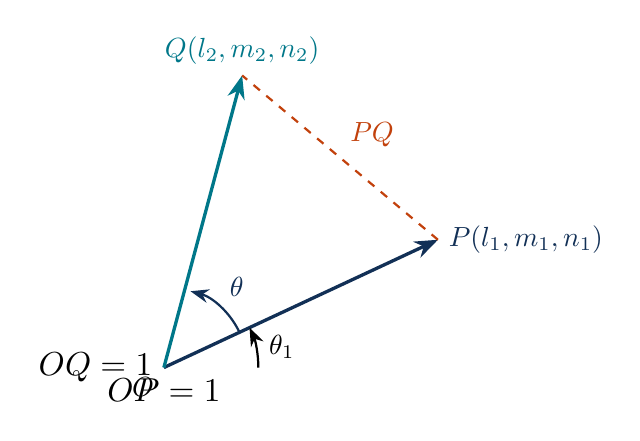
\begin{tikzpicture}[scale=1.2, >=Stealth]
    \coordinate (O) at (0,0);
    \coordinate (P) at (25:3.2);
    \coordinate (Q) at (75:3.2);

    \draw[->, very thick, primary] (O) -- (P) node[right] {$P(l_1, m_1, n_1)$};
    \draw[->, very thick, secondary] (O) -- (Q) node[above] {$Q(l_2, m_2, n_2)$};
    \draw[thick, accent, dashed] (P) -- (Q) node[midway, above right] {$PQ$};

    \draw[->, thick] (1,0) arc (0:25:1) node[midway, right=1pt] {$\theta_1$};
    \draw[->, thick, primary] (0.8, {0.8*tan(25)}) arc (25:75:0.8) node[midway, above right] {$\theta$};

    \node[below left] at (O) {$O$};
    \node[midway, below] at ($(O)!0.5!(P)$) {$OP = 1$};
    \node[midway, left] at ($(O)!0.5!(Q)$) {$OQ = 1$};
\end{tikzpicture}
\end{center}

% =========================================================================
% PAGE 23
% =========================================================================
\section{Page 23: Sine of the Angle, Lagrange's Identity, and Parallelism}
\label{sec:page23}

\begin{conceptbox}[Manuscript Overview: Page 23]
Page 23 derives the formula for $\sin\theta$ between two lines using Lagrange's algebraic identity and establishes the condition for two lines to be parallel in space.
\end{conceptbox}

\subsection{Lagrange's Identity and the Sine Formula}
\begin{theorembox}[Sine of the Angle Between Two Lines]
The sine of the angle $\theta$ between two lines with direction cosines $(l_1, m_1, n_1)$ and $(l_2, m_2, n_2)$ is given by:
\begin{equation}
    \boxed{\sin\theta = \sqrt{(l_1 m_2 - l_2 m_1)^2 + (m_1 n_2 - m_2 n_1)^2 + (n_1 l_2 - n_2 l_1)^2}}
\end{equation}
\end{theorembox}

\begin{proof}
Using $\sin^2\theta = 1 - \cos^2\theta$:
Since $l_1^2+m_1^2+n_1^2 = 1$ and $l_2^2+m_2^2+n_2^2 = 1$, we can write $1$ as their product:
\begin{equation}
    \sin^2\theta = (l_1^2 + m_1^2 + n_1^2)(l_2^2 + m_2^2 + n_2^2) - (l_1 l_2 + m_1 m_2 + n_1 n_2)^2.
\end{equation}
By \textbf{Lagrange's Algebraic Identity}:
For any six real numbers $(A, B, C)$ and $(X, Y, Z)$:
\begin{equation}
    (A^2 + B^2 + C^2)(X^2 + Y^2 + Z^2) - (AX + BY + CZ)^2 = (AY - BX)^2 + (BZ - CY)^2 + (CX - AZ)^2.
\end{equation}
Setting $(A, B, C) = (l_1, m_1, n_1)$ and $(X, Y, Z) = (l_2, m_2, n_2)$:
\begin{equation}
    \sin^2\theta = (l_1 m_2 - l_2 m_1)^2 + (m_1 n_2 - m_2 n_1)^2 + (n_1 l_2 - n_2 l_1)^2.
\end{equation}
Taking the principal square root (since $0 \le \theta \le \pi \implies \sin\theta \ge 0$):
\begin{equation}
    \sin\theta = \sqrt{(l_1 m_2 - l_2 m_1)^2 + (m_1 n_2 - m_2 n_1)^2 + (n_1 l_2 - n_2 l_1)^2}.
\end{equation}
\end{proof}

\subsection{Condition for Parallelism of Two Lines}
Two lines $L_1$ and $L_2$ are parallel if and only if the angle between them is $\theta = 0$ or $\theta = \pi$, which implies $\sin\theta = 0$.
Since $\sin^2\theta$ is the sum of three non-negative squared terms:
\begin{equation}
    (l_1 m_2 - l_2 m_1)^2 + (m_1 n_2 - m_2 n_1)^2 + (n_1 l_2 - n_2 l_1)^2 = 0.
\end{equation}
A sum of squares of real numbers vanishes if and only if each individual term vanishes simultaneously:
\begin{equation}
    l_1 m_2 - l_2 m_1 = 0, \quad m_1 n_2 - m_2 n_1 = 0, \quad n_1 l_2 - n_2 l_1 = 0.
\end{equation}
This yields the celebrated proportionality condition:
\begin{equation}
    \boxed{\frac{l_1}{l_2} = \frac{m_1}{m_2} = \frac{n_1}{n_2}}
\end{equation}
In terms of direction ratios $(a_1, b_1, c_1)$ and $(a_2, b_2, c_2)$:
\begin{equation}
    \boxed{\frac{a_1}{a_2} = \frac{b_1}{b_2} = \frac{c_1}{c_2}}
\end{equation}

% =========================================================================
% PAGE 24
% =========================================================================
\section{Page 24: Solved Problem --- The Four Diagonals of a Cube}
\label{sec:page24}

\begin{conceptbox}[Manuscript Overview: Page 24]
Page 24 presents a classic examination problem: determining the direction cosines of the four body diagonals of a cube and computing the angles between any pair of diagonals, as well as between a diagonal and an edge.
\end{conceptbox}

\begin{examplebox}[Examination Problem: The Diagonals of a Cube]
Prove that the angle between any two diagonals of a cube is $\cos^{-1}\left(\frac{1}{3}\right) \approx 70^\circ 32'$.
\end{examplebox}

\begin{proof}[Complete Step-by-Step Solution]
Let $OABC-DEFG$ be a cube of edge length $a$.
Set the origin at vertex $O(0,0,0)$, and let the three coterminous edges $OA, OC, OD$ lie along the positive directions of the $x$-, $y$-, and $z$-axes respectively.

\begin{center}
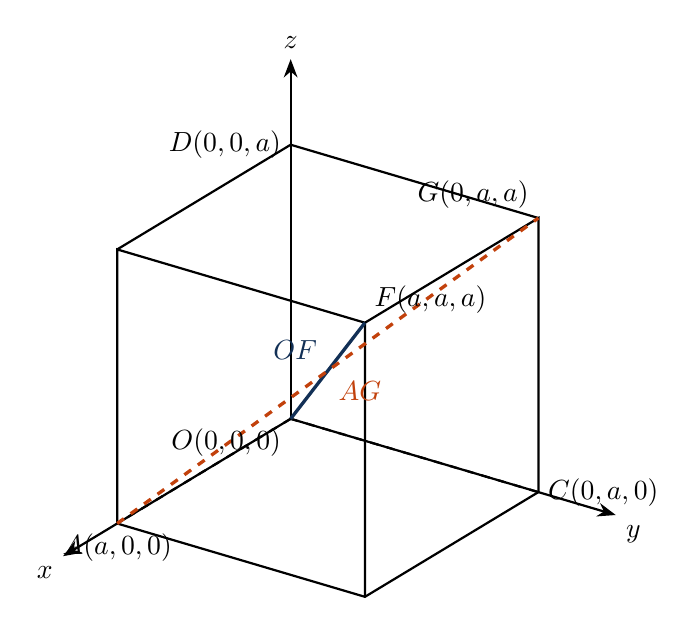
\begin{tikzpicture}[scale=1.2, >=Stealth, 3d view={125}{25}]
    \def\a{3.2}
    % Axes
    \draw[->, thick] (0,0,0) -- (4.2,0,0) node[anchor=north east]{$x$};
    \draw[->, thick] (0,0,0) -- (0,4.2,0) node[anchor=north west]{$y$};
    \draw[->, thick] (0,0,0) -- (0,0,4.2) node[anchor=south]{$z$};

    % Vertices
    \coordinate (O) at (0,0,0);
    \coordinate (A) at (\a,0,0);
    \coordinate (C) at (0,\a,0);
    \coordinate (D) at (0,0,\a);
    \coordinate (B) at (\a,\a,0);
    \coordinate (E) at (\a,0,\a);
    \coordinate (G) at (0,\a,\a);
    \coordinate (F) at (\a,\a,\a);

    % Edges
    \draw[thick] (A) -- (B) -- (C);
    \draw[thick] (A) -- (E) -- (F) -- (B);
    \draw[thick] (C) -- (G) -- (F);
    \draw[thick] (D) -- (E);
    \draw[thick] (D) -- (G);
    \draw[dashed, thick] (O) -- (A);
    \draw[dashed, thick] (O) -- (C);
    \draw[dashed, thick] (O) -- (D);

    % Diagonals
    \draw[very thick, primary] (O) -- (F) node[midway, above left] {$OF$};
    \draw[very thick, accent, dashed] (A) -- (G) node[midway, below right] {$AG$};

    % Nodes
    \node[below left] at (O) {$O(0,0,0)$};
    \node[below] at (A) {$A(a,0,0)$};
    \node[right] at (C) {$C(0,a,0)$};
    \node[left] at (D) {$D(0,0,a)$};
    \node[above right] at (F) {$F(a,a,a)$};
    \node[above left] at (G) {$G(0,a,a)$};
\end{tikzpicture}
\end{center}

The coordinates of the $8$ vertices of the cube are:
\begin{align}
    &O(0,0,0), \quad A(a,0,0), \quad C(0,a,0), \quad D(0,0,a), \nonumber\\
    &B(a,a,0), \quad E(a,0,a), \quad G(0,a,a), \quad F(a,a,a).
\end{align}
The cube possesses $4$ body diagonals connecting opposite pairs of vertices:
\begin{enumerate}
    \item Diagonal $OF$: joins $O(0,0,0)$ to $F(a,a,a)$.
    \begin{align}
        \text{DRs} &= (a - 0, \; a - 0, \; a - 0) = (a, a, a) \sim (1, 1, 1). \nonumber\\
        \text{Length } OF &= \sqrt{a^2 + a^2 + a^2} = a\sqrt{3}. \nonumber\\
        \text{DCs of } OF &= \left(\frac{1}{\sqrt{3}}, \; \frac{1}{\sqrt{3}}, \; \frac{1}{\sqrt{3}}\right).
    \end{align}
    \item Diagonal $AG$: joins $A(a,0,0)$ to $G(0,a,a)$.
    \begin{align}
        \text{DRs} &= (0 - a, \; a - 0, \; a - 0) = (-a, a, a) \sim (-1, 1, 1). \nonumber\\
        \text{DCs of } AG &= \left(-\frac{1}{\sqrt{3}}, \; \frac{1}{\sqrt{3}}, \; \frac{1}{\sqrt{3}}\right).
    \end{align}
    \item Diagonal $BE$: joins $B(a,a,0)$ to $E(0,0,a)$ (or $(a,0,a)$ to $(0,a,0)$):
    \begin{align}
        \text{DRs} &\sim (1, -1, 1). \nonumber\\
        \text{DCs of } BE &= \left(\frac{1}{\sqrt{3}}, \; -\frac{1}{\sqrt{3}}, \; \frac{1}{\sqrt{3}}\right).
    \end{align}
    \item Diagonal $CD$: joins $C(0,a,0)$ to $D(a,a,0)$'s opposite vertex:
    \begin{align}
        \text{DRs} &\sim (1, 1, -1). \nonumber\\
        \text{DCs of } CD &= \left(\frac{1}{\sqrt{3}}, \; \frac{1}{\sqrt{3}}, \; -\frac{1}{\sqrt{3}}\right).
    \end{align}
\end{enumerate}

Now, let $\theta$ be the angle between any two diagonals, say $OF$ and $AG$:
\begin{align}
    \cos\theta &= l_1 l_2 + m_1 m_2 + n_1 n_2 \nonumber\\
    &= \left(\frac{1}{\sqrt{3}}\right)\left(-\frac{1}{\sqrt{3}}\right) + \left(\frac{1}{\sqrt{3}}\right)\left(\frac{1}{\sqrt{3}}\right) + \left(\frac{1}{\sqrt{3}}\right)\left(\frac{1}{\sqrt{3}}\right) \nonumber\\
    &= -\frac{1}{3} + \frac{1}{3} + \frac{1}{3} = \frac{1}{3}.
\end{align}
For any other pair of diagonals, the calculation yields $\pm \frac{1}{3}$. Taking the acute angle between the diagonals:
\begin{equation}
    \boxed{\theta = \cos^{-1}\left(\frac{1}{3}\right) \approx 70^\circ 31' 44''}
\end{equation}
\end{proof}

\begin{notebox}[Angle Between a Body Diagonal and an Edge]
Consider the diagonal $OF$ with DCs $\left(\frac{1}{\sqrt{3}}, \frac{1}{\sqrt{3}}, \frac{1}{\sqrt{3}}\right)$ and the edge $OA$ lying along the $x$-axis with DCs $(1, 0, 0)$.
The angle $\phi$ between them is:
\begin{equation}
    \cos\phi = \left(\frac{1}{\sqrt{3}}\right)(1) + \left(\frac{1}{\sqrt{3}}\right)(0) + \left(\frac{1}{\sqrt{3}}\right)(0) = \frac{1}{\sqrt{3}} \implies \phi = \cos^{-1}\left(\frac{1}{\sqrt{3}}\right) \approx 54^\circ 44'.
\end{equation}
Similarly, the angle $\psi$ between a body diagonal and a face diagonal (e.g., $OB$ with DCs $\left(\frac{1}{\sqrt{2}}, \frac{1}{\sqrt{2}}, 0\right)$) is:
\begin{equation}
    \cos\psi = \left(\frac{1}{\sqrt{3}}\right)\left(\frac{1}{\sqrt{2}}\right) + \left(\frac{1}{\sqrt{3}}\right)\left(\frac{1}{\sqrt{2}}\right) + 0 = \frac{2}{\sqrt{6}} = \sqrt{\frac{2}{3}} \implies \psi = \cos^{-1}\left(\sqrt{\frac{2}{3}}\right) \approx 35^\circ 16'.
\end{equation}
\end{notebox}

\chapter{The Analytical Geometry of the Plane (Pages 25--36)}
\label{ch:the_plane}

% =========================================================================
% PAGE 25
% =========================================================================
\section{Page 25: Definition of a Plane and the General Equation of First Degree}
\label{sec:page25}

\begin{conceptbox}[Manuscript Overview: Page 25]
Page 25 initiates the study of planes in Euclidean space $\mathbb{R}^3$. It establishes the classical geometric definition of a plane, proves that every first-degree algebraic equation in three variables represents a plane, and demonstrates that the general plane equation possesses three independent parameters.
\end{conceptbox}

\subsection{Geometric Definition of a Plane}
\begin{conceptbox}[Geometric Definition of a Plane]
A surface is called a \textbf{plane} if, given any two arbitrary points $P$ and $Q$ on the surface, every point on the straight line segment joining $P$ and $Q$ lies wholly and completely on that surface.
\end{conceptbox}

\subsection{Every First-Degree Equation Represents a Plane}
\begin{theorembox}[General Linear Equation Represents a Plane]
Every algebraic equation of the first degree in $x, y, z$, of the form:
\begin{equation}
    Ax + By + Cz + D = 0
\end{equation}
where $A, B, C$ are not all simultaneously zero ($A^2+B^2+C^2 \neq 0$), represents a plane in three-dimensional space.
\end{theorembox}

\begin{proof}
Let $S$ denote the locus of points whose coordinates satisfy:
\begin{equation}
    Ax + By + Cz + D = 0. \label{eq:plane_gen}
\end{equation}
Let $P(x_1, y_1, z_1)$ and $Q(x_2, y_2, z_2)$ be any two distinct points lying on the surface $S$.
Since $P$ and $Q$ lie on $S$, their coordinates must satisfy equation \eqref{eq:plane_gen}:
\begin{align}
    Ax_1 + By_1 + Cz_1 + D &= 0, \label{eq:pt_P} \\
    Ax_2 + By_2 + Cz_2 + D &= 0. \label{eq:pt_Q}
\end{align}
Now, let $R(x, y, z)$ be any arbitrary point on the straight line passing through $P$ and $Q$.
By the section formula (Page 15), $R$ divides the segment $PQ$ in some real ratio $k : 1$ (where $k \neq -1$):
\begin{equation}
    x = \frac{k x_2 + x_1}{k + 1}, \quad y = \frac{k y_2 + y_1}{k + 1}, \quad z = \frac{k z_2 + z_1}{k + 1}. \label{eq:pt_R_coords}
\end{equation}
To determine whether $R$ lies on the surface $S$, substitute its coordinates into the left-hand side of equation \eqref{eq:plane_gen}:
\begin{align}
    Ax + By + Cz + D &= A\left(\frac{k x_2 + x_1}{k + 1}\right) + B\left(\frac{k y_2 + y_1}{k + 1}\right) + C\left(\frac{k z_2 + z_1}{k + 1}\right) + D \nonumber\\
    &= \frac{1}{k + 1} \Bigl[ k(A x_2 + B y_2 + C z_2 + D) + (A x_1 + B y_1 + C z_1 + D) \Bigr].
\end{align}
Using relations \eqref{eq:pt_P} and \eqref{eq:pt_Q}:
\begin{equation}
    Ax + By + Cz + D = \frac{1}{k + 1} \bigl[ k(0) + (0) \bigr] = 0.
\end{equation}
Thus, the coordinates of $R$ identically satisfy equation \eqref{eq:plane_gen} for \emph{every} value of $k \in \mathbb{R}$.
Consequently, every point on the line $PQ$ lies entirely on the surface.
By the geometric definition, the surface represented by $Ax + By + Cz + D = 0$ is a plane.
\end{proof}

\subsection{Number of Independent Arbitrary Constants}
Although the general equation $Ax + By + Cz + D = 0$ contains four coefficients $A, B, C, D$, dividing through by any non-zero coefficient (say $D \neq 0$) gives:
\begin{equation}
    \left(\frac{A}{D}\right)x + \left(\frac{B}{D}\right)y + \left(\frac{C}{D}\right)z + 1 = 0 \iff a_1 x + b_1 y + c_1 z + 1 = 0.
\end{equation}
Hence, the equation of a plane involves precisely \textbf{three independent arbitrary constants}.
A plane is therefore uniquely determined by three independent geometrical conditions (such as passing through three non-collinear points).

% =========================================================================
% PAGE 26
% =========================================================================
\section{Page 26: Equation of a Plane Passing Through a Given Point}
\label{sec:page26}

\begin{conceptbox}[Manuscript Overview: Page 26]
Page 26 derives the standard one-point form of a plane equation and reveals the geometric significance of the linear coefficients $(A, B, C)$ as the direction ratios of the normal vector to the plane.
\end{conceptbox}

\subsection{One-Point Form of the Plane Equation}
\begin{theorembox}[Plane Passing Through a Given Point]
The general equation of a plane passing through a given point $P_1(x_1, y_1, z_1)$ is:
\begin{equation}
    \boxed{A(x - x_1) + B(y - y_1) + C(z - z_1) = 0}
\end{equation}
where $A, B, C$ are arbitrary constants not all zero.
\end{theorembox}

\begin{proof}
Let the general equation of the plane be:
\begin{equation}
    Ax + By + Cz + D = 0. \label{eq:p26_gen}
\end{equation}
Since the plane passes through $P_1(x_1, y_1, z_1)$, the point satisfies the equation:
\begin{equation}
    Ax_1 + By_1 + Cz_1 + D = 0 \implies D = -(Ax_1 + By_1 + Cz_1). \label{eq:p26_D}
\end{equation}
Subtracting equation \eqref{eq:p26_D} from equation \eqref{eq:p26_gen}:
\begin{equation}
    A(x - x_1) + B(y - y_1) + C(z - z_1) = 0.
\end{equation}
\end{proof}

\subsection{Geometrical Meaning of the Coefficients $(A, B, C)$}
\begin{theorembox}[Normal Vector Theorem]
In the general equation of a plane $Ax + By + Cz + D = 0$, the coefficients $(A, B, C)$ are the direction ratios of the straight line perpendicular (normal) to the plane.
\end{theorembox}

\begin{proof}
Let $P_1(x_1, y_1, z_1)$ and $P_2(x_2, y_2, z_2)$ be any two distinct points lying in the plane $Ax + By + Cz + D = 0$.
The directed line segment $P_1 P_2$ lies completely in the plane. Its direction ratios are:
\begin{equation}
    (x_2 - x_1, \; y_2 - y_1, \; z_2 - z_1).
\end{equation}
Since both points lie on the plane:
\begin{align}
    Ax_1 + By_1 + Cz_1 + D &= 0, \\
    Ax_2 + By_2 + Cz_2 + D &= 0.
\end{align}
Subtracting the first equation from the second:
\begin{equation}
    A(x_2 - x_1) + B(y_2 - y_1) + C(z_2 - z_1) = 0. \label{eq:orthog_plane}
\end{equation}
Comparing equation \eqref{eq:orthog_plane} with the condition of perpendicularity between two directed lines with direction ratios $(a_1,b_1,c_1)$ and $(a_2,b_2,c_2)$, namely $a_1 a_2 + b_1 b_2 + c_1 c_2 = 0$ (Page 21):
Equation \eqref{eq:orthog_plane} proves that a directed line with direction ratios $(A, B, C)$ is perpendicular to the segment $P_1 P_2$.
Since $P_1$ and $P_2$ were arbitrarily chosen in the plane, the vector $\vec{N} = A\,\hat{i} + B\,\hat{j} + C\,\hat{k}$ is perpendicular to \emph{every} line lying in the plane.
Therefore, $(A, B, C)$ are the direction ratios of the normal to the plane.
\end{proof}

% =========================================================================
% PAGE 27
% =========================================================================
\section{Page 27: The Normal Form of the Equation of a Plane}
\label{sec:page27}

\begin{conceptbox}[Manuscript Overview: Page 27]
Page 27 derives the fundamental \textbf{Normal Form} (or Perpendicular Form) of the equation of a plane: $lx + my + nz = p$, where $p$ is the length of the normal from the origin and $(l, m, n)$ are its direction cosines.
\end{conceptbox}

\subsection{Derivation of the Normal Form}
\begin{theorembox}[Normal Form of a Plane]
The equation of a plane at a perpendicular distance $p$ from the origin, whose normal has direction cosines $(l, m, n)$ directed from the origin toward the plane, is:
\begin{equation}
    \boxed{lx + my + nz = p} \quad (p \ge 0)
\end{equation}
\end{theorembox}

\begin{proof}
Let $ON$ be the perpendicular (normal) drawn from the origin $O(0,0,0)$ to the plane.
The length of $ON$ is $p \ge 0$.
Let $(l, m, n)$ be the direction cosines of the directed segment $ON$.
The coordinates of the foot of the perpendicular $N$ are obtained by setting $r = p$ in the projection formulas (Page 17):
\begin{equation}
    N = (lp, \; mp, \; np).
\end{equation}
Let $P(x, y, z)$ be any arbitrary point on the plane. Join $NP$.

\begin{center}
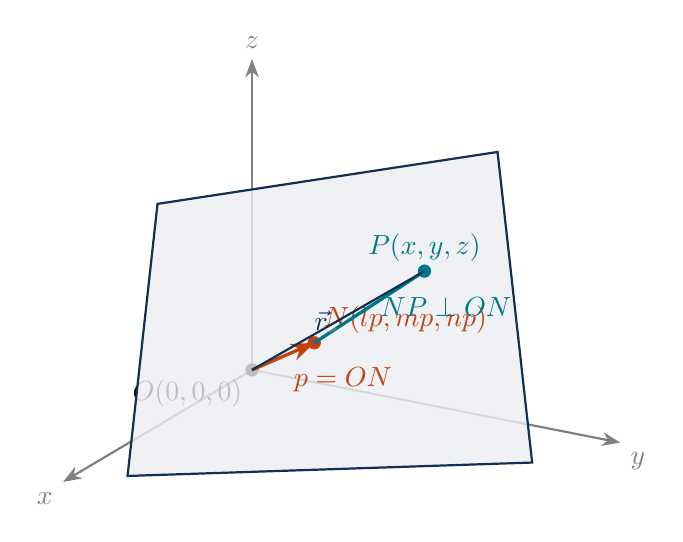
\begin{tikzpicture}[scale=1.2, >=Stealth, 3d view={120}{20}]
    % Coordinate axes
    \draw[->, thick, gray] (0,0,0) -- (4,0,0) node[anchor=north east]{$x$};
    \draw[->, thick, gray] (0,0,0) -- (0,4.5,0) node[anchor=north west]{$y$};
    \draw[->, thick, gray] (0,0,0) -- (0,0,3.5) node[anchor=south]{$z$};

    % Origin
    \coordinate (O) at (0,0,0);
    \node[below left] at (O) {$O(0,0,0)$};
    \fill (O) circle (2pt);

    % Plane patch
    \coordinate (V1) at (3.5, 0.5, 0);
    \coordinate (V2) at (1.0, 4.0, 0);
    \coordinate (V3) at (0, 3.0, 3.0);
    \coordinate (V4) at (2.0, 0, 2.5);
    \fill[primary!8, opacity=0.8] (V1) -- (V2) -- (V3) -- (V4) -- cycle;
    \draw[thick, primary] (V1) -- (V2) -- (V3) -- (V4) -- cycle;

    % Normal ON
    \coordinate (N) at (1.8, 1.8, 1.2);
    \draw[very thick, accent, ->] (O) -- (N) node[midway, below right] {$p = ON$};
    \fill[accent] (N) circle (2pt) node[above right] {$N(lp, mp, np)$};

    % Point P
    \coordinate (P) at (1.2, 2.8, 2.0);
    \fill[secondary] (P) circle (2pt) node[above] {$P(x,y,z)$};

    % Line NP in plane
    \draw[very thick, secondary] (N) -- (P) node[midway, right] {$NP \perp ON$};
    \draw[thick, primary] (O) -- (P) node[midway, left] {$\vec{r}$};

    % Right angle marker
    \draw[dashed, gray] ($(N)!0.2!(P)$) -- ++($(N)!0.2!(O)-(N)$);
\end{tikzpicture}
\end{center}

Since $ON$ is perpendicular to the entire plane, it is perpendicular to every line lying in the plane through $N$.
In particular, $ON \perp NP$, so the triangle $\triangle ONP$ is right-angled at $N$.
By the Pythagorean theorem or orthogonality:
The direction ratios of $NP$ are $(x - lp, \; y - mp, \; z - np)$.
The direction cosines of $ON$ are $(l, m, n)$.
Applying the condition of perpendicularity:
\begin{align}
    l(x - lp) + m(y - mp) + n(z - np) &= 0 \nonumber\\
    lx + my + nz - p(l^2 + m^2 + n^2) &= 0.
\end{align}
Since $(l, m, n)$ are direction cosines, $l^2 + m^2 + n^2 = 1$. Therefore:
\begin{equation}
    \boxed{lx + my + nz = p}
\end{equation}
\end{proof}

% =========================================================================
% PAGE 28
% =========================================================================
\section{Page 28: Reduction of the General Equation to the Normal Form}
\label{sec:page28}

\begin{conceptbox}[Manuscript Overview: Page 28]
Page 28 addresses the algorithmic reduction of any given first-degree equation $Ax + By + Cz + D = 0$ into the canonical normal form $lx + my + nz = p$, rigorously establishing the sign conventions ensuring $p \ge 0$.
\end{conceptbox}

\subsection{The Reduction Algorithm}
Let the general equation of a plane be:
\begin{equation}
    Ax + By + Cz + D = 0 \iff Ax + By + Cz = -D. \label{eq:p28_gen}
\end{equation}
We wish to express this in the normal form:
\begin{equation}
    lx + my + nz = p \quad (p \ge 0). \label{eq:p28_norm}
\end{equation}
Equations \eqref{eq:p28_gen} and \eqref{eq:p28_norm} represent the exact same plane if and only if their corresponding coefficients are strictly proportional:
\begin{equation}
    \frac{l}{A} = \frac{m}{B} = \frac{n}{C} = \frac{p}{-D} = k.
\end{equation}
From this proportionality:
\begin{equation}
    l = kA, \quad m = kB, \quad n = kC, \quad p = -kD.
\end{equation}
Squaring and adding the direction cosines:
\begin{equation}
    l^2 + m^2 + n^2 = k^2(A^2 + B^2 + C^2) \implies 1 = k^2(A^2 + B^2 + C^2).
\end{equation}
Hence, the multiplier $k$ is:
\begin{equation}
    k = \pm \frac{1}{\sqrt{A^2 + B^2 + C^2}}.
\end{equation}

\subsection{Sign Convention for the Perpendicular Distance $p \ge 0$}
Since $p$ is a geometric length ($p \ge 0$), the sign of $k$ must be chosen so that $p = -kD \ge 0$:
\begin{itemize}
    \item \textbf{Case 1 ($D < 0$)}: If the constant term $D$ is negative, then $-D > 0$. We choose the positive root:
    \begin{equation}
        k = +\frac{1}{\sqrt{A^2 + B^2 + C^2}}.
    \end{equation}
    \item \textbf{Case 2 ($D > 0$)}: If the constant term $D$ is positive, then $-D < 0$. To make $p$ positive, we must choose the negative root:
    \begin{equation}
        k = -\frac{1}{\sqrt{A^2 + B^2 + C^2}}.
    \end{equation}
\end{itemize}

\begin{theorembox}[Normalized Plane Parameters]
For any plane $Ax + By + Cz + D = 0$:
\begin{enumerate}
    \item The perpendicular distance from the origin is:
    \begin{equation}
        \boxed{p = \frac{|D|}{\sqrt{A^2 + B^2 + C^2}}}
    \end{equation}
    \item The direction cosines of the normal from the origin to the plane are:
    \begin{equation}
        \boxed{l = \frac{\mp A}{\sqrt{A^2 + B^2 + C^2}}, \quad m = \frac{\mp B}{\sqrt{A^2 + B^2 + C^2}}, \quad n = \frac{\mp C}{\sqrt{A^2 + B^2 + C^2}}}
    \end{equation}
    where the sign is chosen opposite to the sign of $D$.
\end{enumerate}
\end{theorembox}

% =========================================================================
% PAGE 29
% =========================================================================
\section{Page 29: Intercept Form and the Three-Point Determinant Form}
\label{sec:page29}

\begin{conceptbox}[Manuscript Overview: Page 29]
Page 29 derives two essential representations of a plane:
\begin{enumerate}[noitemsep]
    \item The \textbf{Intercept Form}, expressing the plane via its intercepts $(a, b, c)$ on the axes.
    \item The \textbf{Three-Point Determinant Form}, establishing the unique plane passing through three non-collinear spatial points.
\end{enumerate}
\end{conceptbox}

\subsection{The Intercept Form of a Plane}
\begin{theorembox}[Intercept Form]
The equation of a plane making non-zero intercepts $a, b, c$ on the coordinate axes $OX, OY, OZ$ respectively is:
\begin{equation}
    \boxed{\frac{x}{a} + \frac{y}{b} + \frac{z}{c} = 1}
\end{equation}
\end{theorembox}

\begin{proof}
Let the plane meet the coordinate axes at $A(a, 0, 0)$, $B(0, b, 0)$, and $C(0, 0, c)$.
Let the general equation of the plane be $Ax + By + Cz + D = 0$.
Since $A, B, C$ lie on the plane:
\begin{align}
    A(a) + B(0) + C(0) + D = 0 &\implies Aa + D = 0 \implies A = -\frac{D}{a}, \\
    A(0) + B(b) + C(0) + D = 0 &\implies Bb + D = 0 \implies B = -\frac{D}{b}, \\
    A(0) + B(0) + C(c) + D = 0 &\implies Cc + D = 0 \implies C = -\frac{D}{c}.
\end{align}
Substituting these into the general equation:
\begin{equation}
    -\frac{D}{a}x - \frac{D}{b}y - \frac{D}{c}z + D = 0.
\end{equation}
Dividing by $-D$ (since $D \neq 0$ for non-zero intercepts):
\begin{equation}
    \boxed{\frac{x}{a} + \frac{y}{b} + \frac{z}{c} = 1}
\end{equation}
\end{proof}

\begin{center}
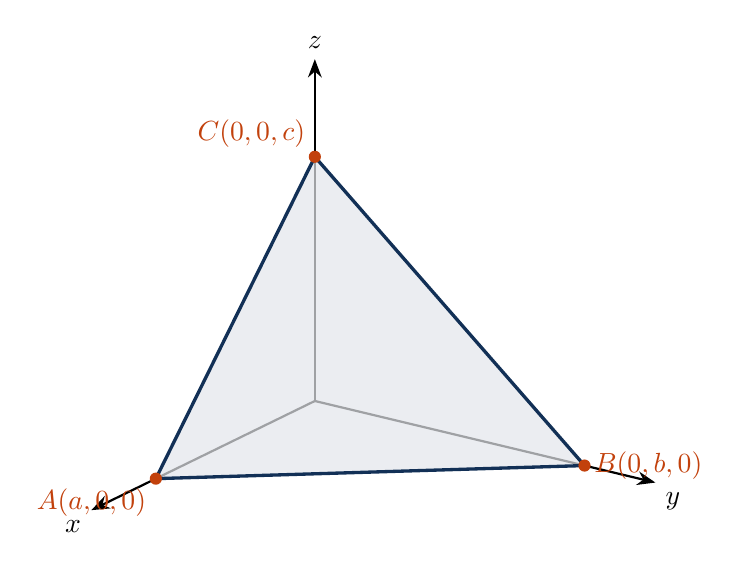
\begin{tikzpicture}[scale=1.1, >=Stealth, 3d view={125}{20}]
    \draw[->, thick] (0,0,0) -- (4.5,0,0) node[anchor=north east]{$x$};
    \draw[->, thick] (0,0,0) -- (0,4.8,0) node[anchor=north west]{$y$};
    \draw[->, thick] (0,0,0) -- (0,0,4.2) node[anchor=south]{$z$};

    \coordinate (O) at (0,0,0);
    \coordinate (A) at (3.2,0,0);
    \coordinate (B) at (0,3.8,0);
    \coordinate (C) at (0,0,3.0);

    % Intercept triangle
    \fill[primary!12, opacity=0.7] (A) -- (B) -- (C) -- cycle;
    \draw[very thick, primary] (A) -- (B) node[midway, below] {};
    \draw[very thick, primary] (B) -- (C);
    \draw[very thick, primary] (C) -- (A);

    \fill[accent] (A) circle (2pt) node[below left] {$A(a,0,0)$};
    \fill[accent] (B) circle (2pt) node[right] {$B(0,b,0)$};
    \fill[accent] (C) circle (2pt) node[above left] {$C(0,0,c)$};
\end{tikzpicture}
\end{center}

\subsection{Plane Through Three Non-Collinear Points}
\begin{theorembox}[Three-Point Determinant Form]
The equation of the plane passing through three non-collinear points $P_1(x_1, y_1, z_1)$, $P_2(x_2, y_2, z_2)$, and $P_3(x_3, y_3, z_3)$ is:
\begin{equation}
    \boxed{\begin{vmatrix}
    x & y & z & 1 \\
    x_1 & y_1 & z_1 & 1 \\
    x_2 & y_2 & z_2 & 1 \\
    x_3 & y_3 & z_3 & 1
    \end{vmatrix} = 0 \iff
    \begin{vmatrix}
    x - x_1 & y - y_1 & z - z_1 \\
    x_2 - x_1 & y_2 - y_1 & z_2 - z_1 \\
    x_3 - x_1 & y_3 - y_1 & z_3 - z_1
    \end{vmatrix} = 0}
\end{equation}
\end{theorembox}

\begin{proof}
The general plane through $P_1(x_1, y_1, z_1)$ is:
\begin{equation}
    A(x - x_1) + B(y - y_1) + C(z - z_1) = 0. \label{eq:p29_onept}
\end{equation}
Since $P_2$ and $P_3$ also lie on the plane:
\begin{align}
    A(x_2 - x_1) + B(y_2 - y_1) + C(z_2 - z_1) &= 0, \label{eq:p29_pt2} \\
    A(x_3 - x_1) + B(y_3 - y_1) + C(z_3 - z_1) &= 0. \label{eq:p29_pt3}
\end{align}
Equations \eqref{eq:p29_onept}, \eqref{eq:p29_pt2}, and \eqref{eq:p29_pt3} form a homogeneous linear system in the unknowns $A, B, C$.
For non-trivial solutions $(A, B, C) \neq (0, 0, 0)$ to exist, the determinant of the coefficient matrix must vanish:
\begin{equation}
    \begin{vmatrix}
    x - x_1 & y - y_1 & z - z_1 \\
    x_2 - x_1 & y_2 - y_1 & z_2 - z_1 \\
    x_3 - x_1 & y_3 - y_1 & z_3 - z_1
    \end{vmatrix} = 0.
\end{equation}
\end{proof}

% =========================================================================
% PAGE 30
% =========================================================================
\section{Page 30: Solved Examination Problems on Plane Equations}
\label{sec:page30}

\begin{conceptbox}[Manuscript Overview: Page 30]
Page 30 works through standard university examination problems illustrating the application of the three-point determinant form and the intercept relations.
\end{conceptbox}

\begin{examplebox}[Problem 1: Plane Through Three Given Points]
Find the Cartesian equation of the plane passing through the three points:
\begin{equation}
    P_1(2, 2, -1), \quad P_2(3, 4, 2), \quad P_3(7, 0, 6).
\end{equation}
\end{examplebox}

\begin{proof}[Step-by-Step Analytical Solution]
We apply the three-point determinant formula with $(x_1, y_1, z_1) = (2, 2, -1)$:
\begin{equation}
    \begin{vmatrix}
    x - 2 & y - 2 & z - (-1) \\
    3 - 2 & 4 - 2 & 2 - (-1) \\
    7 - 2 & 0 - 2 & 6 - (-1)
    \end{vmatrix} = 0.
\end{equation}
Simplifying the numerical entries in rows 2 and 3:
\begin{equation}
    \begin{vmatrix}
    x - 2 & y - 2 & z + 1 \\
    1 & 2 & 3 \\
    5 & -2 & 7
    \end{vmatrix} = 0.
\end{equation}
Expanding the determinant along the first row:
\begin{align}
    (x - 2) \begin{vmatrix} 2 & 3 \\ -2 & 7 \end{vmatrix}
    - (y - 2) \begin{vmatrix} 1 & 3 \\ 5 & 7 \end{vmatrix}
    + (z + 1) \begin{vmatrix} 1 & 2 \\ 5 & -2 \end{vmatrix} &= 0.
\end{align}
Evaluating each $2 \times 2$ minor:
\begin{align}
    \begin{vmatrix} 2 & 3 \\ -2 & 7 \end{vmatrix} &= (2)(7) - (3)(-2) = 14 + 6 = 20, \\
    \begin{vmatrix} 1 & 3 \\ 5 & 7 \end{vmatrix} &= (1)(7) - (3)(5) = 7 - 15 = -8, \\
    \begin{vmatrix} 1 & 2 \\ 5 & -2 \end{vmatrix} &= (1)(-2) - (2)(5) = -2 - 10 = -12.
\end{align}
Substituting the minors back:
\begin{align}
    20(x - 2) - (-8)(y - 2) + (-12)(z + 1) &= 0 \nonumber\\
    20(x - 2) + 8(y - 2) - 12(z + 1) &= 0.
\end{align}
Expanding the brackets:
\begin{align}
    20x - 40 + 8y - 16 - 12z - 12 &= 0 \nonumber\\
    20x + 8y - 12z - 68 &= 0.
\end{align}
Dividing throughout by the common factor $4$:
\begin{equation}
    \boxed{5x + 2y - 3z - 17 = 0}
\end{equation}
\textbf{Verification}:
\begin{itemize}[noitemsep]
    \item Point $P_1(2, 2, -1)$: $5(2) + 2(2) - 3(-1) - 17 = 10 + 4 + 3 - 17 = 0$ \quad \checkmark
    \item Point $P_2(3, 4, 2)$: $5(3) + 2(4) - 3(2) - 17 = 15 + 8 - 6 - 17 = 0$ \quad \checkmark
    \item Point $P_3(7, 0, 6)$: $5(7) + 2(0) - 3(6) - 17 = 35 + 0 - 18 - 17 = 0$ \quad \checkmark
\end{itemize}
\end{proof}

% =========================================================================
% PAGE 31
% =========================================================================
\section{Page 31: Perpendicular Distance of a Point from a Plane}
\label{sec:page31}

\begin{conceptbox}[Manuscript Overview: Page 31]
Page 31 derives the formula for the perpendicular distance of a given point $P(x_1, y_1, z_1)$ from an arbitrary plane $Ax + By + Cz + D = 0$.
\end{conceptbox}

\subsection{Derivation of the Distance Formula}
\begin{theorembox}[Perpendicular Distance of a Point from a Plane]
The perpendicular distance $d$ from the point $P(x_1, y_1, z_1)$ to the plane $Ax + By + Cz + D = 0$ is:
\begin{equation}
    \boxed{d = \frac{|Ax_1 + By_1 + Cz_1 + D|}{\sqrt{A^2 + B^2 + C^2}}}
\end{equation}
\end{theorembox}

\begin{proof}
First, transform the plane equation into normal form:
\begin{equation}
    lx + my + nz - p = 0
\end{equation}
where $l = \frac{A}{\sqrt{\sum A^2}}, m = \frac{B}{\sqrt{\sum A^2}}, n = \frac{C}{\sqrt{\sum A^2}}$, and $p = \frac{-D}{\sqrt{\sum A^2}}$.
Draw a plane parallel to the given plane passing through $P(x_1, y_1, z_1)$.
Since it is parallel, it possesses the identical normal direction cosines $(l, m, n)$. Its equation is:
\begin{equation}
    lx + my + nz = p'
\end{equation}
where $p'$ is the perpendicular distance of this parallel plane from the origin.
Since $P(x_1, y_1, z_1)$ lies on this parallel plane:
\begin{equation}
    p' = lx_1 + my_1 + nz_1.
\end{equation}
The perpendicular distance $d$ from $P$ to the original plane is simply the distance between the two parallel planes:
\begin{equation}
    d = |p' - p| = |lx_1 + my_1 + nz_1 - p|.
\end{equation}
Substituting the expressions for $l, m, n, p$:
\begin{align}
    d &= \left| \frac{A}{\sqrt{A^2+B^2+C^2}}x_1 + \frac{B}{\sqrt{A^2+B^2+C^2}}y_1 + \frac{C}{\sqrt{A^2+B^2+C^2}}z_1 - \left(\frac{-D}{\sqrt{A^2+B^2+C^2}}\right) \right| \nonumber\\
    &= \frac{|Ax_1 + By_1 + Cz_1 + D|}{\sqrt{A^2 + B^2 + C^2}}.
\end{align}
\end{proof}

\subsection{Distance Between Two Parallel Planes}
If two planes are parallel, their linear terms can be scaled to be identical:
\begin{equation}
    \Pi_1: Ax + By + Cz + D_1 = 0, \quad \Pi_2: Ax + By + Cz + D_2 = 0.
\end{equation}
The perpendicular distance between them is:
\begin{equation}
    \boxed{d = \frac{|D_1 - D_2|}{\sqrt{A^2 + B^2 + C^2}}}
\end{equation}

% =========================================================================
% PAGE 32
% =========================================================================
\section{Page 32: Position of Points Relative to a Plane and Systems of Planes}
\label{sec:page32}

\begin{conceptbox}[Manuscript Overview: Page 32]
Page 32 analyzes:
\begin{enumerate}[noitemsep]
    \item The relative position of two points with respect to a plane (whether they lie on the same side or opposite sides).
    \item The one-parameter family of planes passing through the line of intersection of two given planes ($U + \lambda V = 0$).
\end{enumerate}
\end{conceptbox}

\subsection{Position of Two Points Relative to a Plane}
\begin{theorembox}[Same Side vs. Opposite Sides Criterion]
Two points $P(x_1, y_1, z_1)$ and $Q(x_2, y_2, z_2)$ lie on the \textbf{same side} or \textbf{opposite sides} of the plane $\Pi: Ax + By + Cz + D = 0$ according to whether the expressions:
\begin{equation}
    Ax_1 + By_1 + Cz_1 + D \quad \text{and} \quad Ax_2 + By_2 + Cz_2 + D
\end{equation}
have the \textbf{same sign} or \textbf{opposite signs}.
\end{theorembox}

\begin{proof}
Let the segment $PQ$ meet the plane $\Pi$ at point $R$.
Let $R$ divide $PQ$ in the ratio $k : 1$. The coordinates of $R$ are:
\begin{equation}
    R = \left(\frac{kx_2 + x_1}{k + 1}, \; \frac{ky_2 + y_1}{k + 1}, \; \frac{kz_2 + z_1}{k + 1}\right).
\end{equation}
Since $R$ lies on the plane $Ax + By + Cz + D = 0$:
\begin{align}
    A\left(\frac{kx_2 + x_1}{k+1}\right) + B\left(\frac{ky_2 + y_1}{k+1}\right) + C\left(\frac{kz_2 + z_1}{k+1}\right) + D &= 0 \nonumber\\
    k(Ax_2 + By_2 + Cz_2 + D) + (Ax_1 + By_1 + Cz_1 + D) &= 0 \nonumber\\
    \implies k &= -\frac{Ax_1 + By_1 + Cz_1 + D}{Ax_2 + By_2 + Cz_2 + D}.
\end{align}
\begin{itemize}
    \item If $k > 0$, the division is internal $\implies$ $R$ lies strictly between $P$ and $Q$ $\implies P$ and $Q$ lie on \textbf{opposite sides} of the plane. This requires $\frac{Ax_1+By_1+Cz_1+D}{Ax_2+By_2+Cz_2+D} < 0$, i.e., they have \textbf{opposite signs}.
    \item If $k < 0$, the division is external $\implies R$ does not lie between $P$ and $Q$ $\implies P$ and $Q$ lie on the \textbf{same side} of the plane. This requires $\frac{Ax_1+By_1+Cz_1+D}{Ax_2+By_2+Cz_2+D} > 0$, i.e., they have the \textbf{same sign}.
\end{itemize}
\end{proof}

\subsection{Plane Passing Through the Intersection of Two Given Planes}
\begin{theorembox}[Family of Planes $U + \lambda V = 0$]
Let $U \equiv A_1 x + B_1 y + C_1 z + D_1 = 0$ and $V \equiv A_2 x + B_2 y + C_2 z + D_2 = 0$ be two intersecting planes.
The equation of any plane passing through their line of intersection is given by:
\begin{equation}
    \boxed{U + \lambda V = 0 \iff (A_1 x + B_1 y + C_1 z + D_1) + \lambda(A_2 x + B_2 y + C_2 z + D_2) = 0}
\end{equation}
where $\lambda$ is an arbitrary scalar parameter ($-\infty < \lambda < \infty$).
\end{theorembox}

\begin{proof}
\begin{enumerate}
    \item Equation $U + \lambda V = 0$ is of the first degree in $x, y, z$:
    \begin{equation}
        (A_1 + \lambda A_2)x + (B_1 + \lambda B_2)y + (C_1 + \lambda C_2)z + (D_1 + \lambda D_2) = 0.
    \end{equation}
    By Page 25, this represents a plane for every value of $\lambda$.
    \item Any point $(x_0, y_0, z_0)$ lying on the line of intersection of $U=0$ and $V=0$ satisfies $U(x_0, y_0, z_0) = 0$ and $V(x_0, y_0, z_0) = 0$.
    Consequently, $U(x_0, y_0, z_0) + \lambda V(x_0, y_0, z_0) = 0 + \lambda(0) = 0$.
    Thus, the plane contains every point of the line of intersection.
\end{enumerate}
\end{proof}

% =========================================================================
% PAGE 33
% =========================================================================
\section{Page 33: Planes Bisecting the Dihedral Angles Between Two Planes}
\label{sec:page33}

\begin{conceptbox}[Manuscript Overview: Page 33]
Page 33 investigates the geometry of dihedral angles between two non-parallel planes and derives the algebraic equations representing the pair of planes that bisect these dihedral angles.
\end{conceptbox}

\subsection{Definition and Geometric Derivation}
Let two non-parallel planes be:
\begin{align}
    \Pi_1 &: A_1 x + B_1 y + C_1 z + D_1 = 0, \\
    \Pi_2 &: A_2 x + B_2 y + C_2 z + D_2 = 0.
\end{align}
A point $P(x, y, z)$ lies on a plane bisecting the dihedral angle between $\Pi_1$ and $\Pi_2$ if and only if it is \textbf{equidistant} from both planes.

\begin{center}
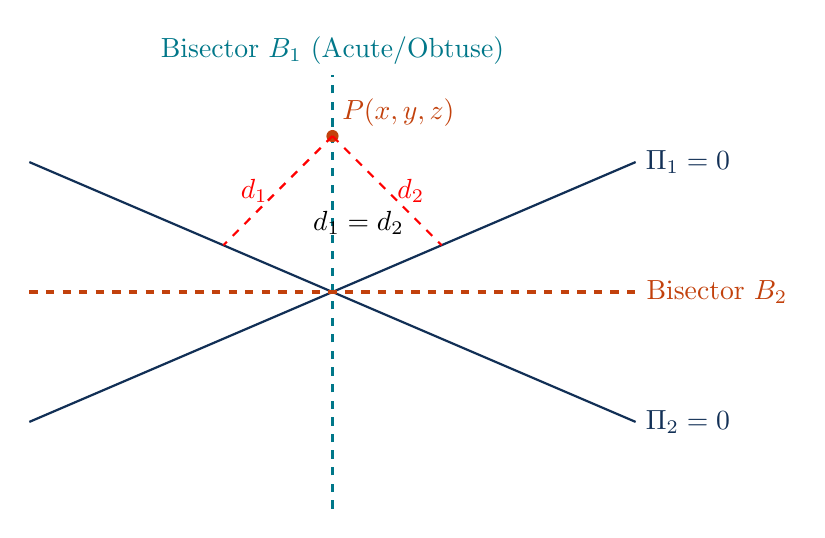
\begin{tikzpicture}[scale=1.1, >=Stealth]
    % Intersecting planes in cross section
    \draw[thick, primary] (-3.5,-1.5) -- (3.5,1.5) node[right] {$\Pi_1 = 0$};
    \draw[thick, primary] (-3.5,1.5) -- (3.5,-1.5) node[right] {$\Pi_2 = 0$};

    % Bisectors
    \draw[very thick, secondary, dashed] (0,-2.5) -- (0,2.5) node[above] {Bisector $B_1$ (Acute/Obtuse)};
    \draw[very thick, accent, dashed] (-3.5,0) -- (3.5,0) node[right] {Bisector $B_2$};

    % Point P on bisector
    \coordinate (P) at (0, 1.8);
    \fill[accent] (P) circle (2pt) node[above right] {$P(x,y,z)$};

    % Perpendiculars to planes
    \draw[dashed, red, thick] (P) -- (-1.26, 0.54) node[midway, left] {$d_1$};
    \draw[dashed, red, thick] (P) -- (1.26, 0.54) node[midway, right] {$d_2$};

    \node at (0.3, 0.8) {$d_1 = d_2$};
\end{tikzpicture}
\end{center}

Applying the perpendicular distance formula (Page 31):
\begin{align}
    d_1 &= \frac{|A_1 x + B_1 y + C_1 z + D_1|}{\sqrt{A_1^2 + B_1^2 + C_1^2}}, \\
    d_2 &= \frac{|A_2 x + B_2 y + C_2 z + D_2|}{\sqrt{A_2^2 + B_2^2 + C_2^2}}.
\end{align}
Setting $d_1 = d_2$:
\begin{equation}
    \frac{|A_1 x + B_1 y + C_1 z + D_1|}{\sqrt{A_1^2 + B_1^2 + C_1^2}} = \frac{|A_2 x + B_2 y + C_2 z + D_2|}{\sqrt{A_2^2 + B_2^2 + C_2^2}}.
\end{equation}
Removing the absolute value signs yields the two bisecting planes:
\begin{equation}
    \boxed{\frac{A_1 x + B_1 y + C_1 z + D_1}{\sqrt{A_1^2 + B_1^2 + C_1^2}} = \pm \frac{A_2 x + B_2 y + C_2 z + D_2}{\sqrt{A_2^2 + B_2^2 + C_2^2}}}
\end{equation}

\subsection{Orthogonality of the Two Bisector Planes}
\begin{theorembox}[Mutual Perpendicularity of Angle Bisectors]
The two bisector planes corresponding to the $+$ and $-$ signs are mutually perpendicular.
\end{theorembox}

\begin{proof}
Let $k_1 = \sqrt{A_1^2+B_1^2+C_1^2}$ and $k_2 = \sqrt{A_2^2+B_2^2+C_2^2}$.
The equations of the two planes can be written as:
\begin{align}
    B^+ &: \left(\frac{A_1}{k_1} - \frac{A_2}{k_2}\right)x + \left(\frac{B_1}{k_1} - \frac{B_2}{k_2}\right)y + \left(\frac{C_1}{k_1} - \frac{C_2}{k_2}\right)z + \left(\frac{D_1}{k_1} - \frac{D_2}{k_2}\right) = 0, \\
    B^- &: \left(\frac{A_1}{k_1} + \frac{A_2}{k_2}\right)x + \left(\frac{B_1}{k_1} + \frac{B_2}{k_2}\right)y + \left(\frac{C_1}{k_1} + \frac{C_2}{k_2}\right)z + \left(\frac{D_1}{k_1} + \frac{D_2}{k_2}\right) = 0.
\end{align}
The scalar dot product of their normal vectors $\vec{N}_1$ and $\vec{N}_2$ is:
\begin{align}
    \vec{N}_1 \cdot \vec{N}_2 &= \left(\frac{A_1}{k_1} - \frac{A_2}{k_2}\right)\left(\frac{A_1}{k_1} + \frac{A_2}{k_2}\right) + \left(\frac{B_1}{k_1} - \frac{B_2}{k_2}\right)\left(\frac{B_1}{k_1} + \frac{B_2}{k_2}\right) + \left(\frac{C_1}{k_1} - \frac{C_2}{k_2}\right)\left(\frac{C_1}{k_1} + \frac{C_2}{k_2}\right) \nonumber\\
    &= \left(\frac{A_1^2}{k_1^2} - \frac{A_2^2}{k_2^2}\right) + \left(\frac{B_1^2}{k_1^2} - \frac{B_2^2}{k_2^2}\right) + \left(\frac{C_1^2}{k_1^2} - \frac{C_2^2}{k_2^2}\right) \nonumber\\
    &= \frac{A_1^2 + B_1^2 + C_1^2}{k_1^2} - \frac{A_2^2 + B_2^2 + C_2^2}{k_2^2} = \frac{k_1^2}{k_1^2} - \frac{k_2^2}{k_2^2} = 1 - 1 = \boxed{0}.
\end{align}
Since $\vec{N}_1 \cdot \vec{N}_2 = 0$, the two bisecting planes are perpendicular to each other.
\end{proof}

% =========================================================================
% PAGE 34
% =========================================================================
\section{Page 34: Discrimination Between Acute and Obtuse Angle Bisectors}
\label{sec:page34}

\begin{conceptbox}[Manuscript Overview: Page 34]
Page 34 establishes the rigorous analytical criteria used to distinguish between the \textbf{acute angle bisector} and the \textbf{obtuse angle bisector}, as well as identifying which bisector contains the origin.
\end{conceptbox}

\subsection{The Standard University Algorithm}
To systematically classify the bisectors:
\begin{enumerate}
    \item \textbf{Standardize Constant Terms}:
    Write both plane equations such that their constant terms are \textbf{strictly positive}:
    \begin{align}
        A_1 x + B_1 y + C_1 z + D_1 &= 0 \quad (D_1 > 0), \\
        A_2 x + B_2 y + C_2 z + D_2 &= 0 \quad (D_2 > 0).
    \end{align}
    (If any constant term is negative, multiply that entire equation by $-1$).
    \item \textbf{Bisector Containing the Origin}:
    With $D_1 > 0$ and $D_2 > 0$, the origin $(0,0,0)$ substituted into both planes yields positive values ($D_1 > 0$ and $D_2 > 0$).
    Therefore, the origin lies in the region where both plane expressions have the same sign.
    Hence, the \textbf{bisector containing the origin} is given by the \textbf{positive ($+$) sign}:
    \begin{equation}
        \boxed{\frac{A_1 x + B_1 y + C_1 z + D_1}{\sqrt{A_1^2 + B_1^2 + C_1^2}} = +\frac{A_2 x + B_2 y + C_2 z + D_2}{\sqrt{A_2^2 + B_2^2 + C_2^2}}}
    \end{equation}
    The bisector not containing the origin is given by the negative ($-$) sign.
    \item \textbf{Evaluate the Coefficient Scalar Product}:
    Calculate the sum of products of direction coefficients:
    \begin{equation}
        \Delta = A_1 A_2 + B_1 B_2 + C_1 C_2.
    \end{equation}
\end{enumerate}

\begin{theorembox}[Classification Criterion for Acute and Obtuse Bisectors]
Provided $D_1 > 0$ and $D_2 > 0$:
\begin{center}
\begin{tabular}{|c|c|c|}
\hline
\textbf{Sign of } $\Delta = A_1 A_2 + B_1 B_2 + C_1 C_2$ & \textbf{Origin Lies In} & \textbf{Acute Angle Bisector} \\
\hline
$\Delta > 0$ & Obtuse Angle & Negative ($-$) sign \\
$\Delta < 0$ & Acute Angle & Positive ($+$) sign \\
\hline
\end{tabular}
\end{center}
\end{theorembox}

\begin{proof}
Let $\theta$ be the angle between the normal vectors $\vec{N}_1 = (A_1, B_1, C_1)$ and $\vec{N}_2 = (A_2, B_2, C_2)$ directed away from the origin:
\begin{equation}
    \cos\theta = \frac{A_1 A_2 + B_1 B_2 + C_1 C_2}{\sqrt{\sum A_1^2}\sqrt{\sum A_2^2}}.
\end{equation}
\begin{itemize}
    \item If $\Delta > 0 \implies \cos\theta > 0 \implies \theta$ is acute $\implies$ the angle between the planes containing the origin is supplementary to $\theta$, i.e., $180^\circ - \theta$, which is \textbf{obtuse}.
    Thus, the origin lies in the obtuse angle.
    The positive sign (which contains the origin) bisects the obtuse angle, and the negative sign bisects the acute angle.
    \item If $\Delta < 0 \implies \cos\theta < 0 \implies \theta$ is obtuse $\implies 180^\circ - \theta$ is \textbf{acute}.
    Thus, the origin lies in the acute angle.
    The positive sign bisects the acute angle, and the negative sign bisects the obtuse angle.
\end{itemize}
\end{proof}

% =========================================================================
% PAGE 35
% =========================================================================
\section{Page 35: Method 2 (Point Method) and Comprehensive Worked Problem}
\label{sec:page35}

\begin{conceptbox}[Manuscript Overview: Page 35]
Page 35 presents the alternative geometric method (the \textbf{Point Method} or Tangent Half-Angle Method) for verifying the nature of a bisector, followed by a complete numerical examination problem.
\end{conceptbox}

\subsection{Method 2: The Tangent Half-Angle (Point) Method}
If one is unsure of the sign convention, the following constructive procedure can be used:
\begin{enumerate}
    \item Obtain the two bisector planes $B_1$ and $B_2$.
    \item Choose any convenient point $P$ on one of the bisector planes (say $B_1$).
    \item Calculate the perpendicular distance $p$ from $P$ to one of the original planes $\Pi_1$.
    \item Calculate the distance $r$ from $P$ to the line of intersection of the two planes.
    \item If $\theta$ is the dihedral angle between the original planes, then in the right triangle formed by $P$, its projection on $\Pi_1$, and its projection on the intersection line:
    \begin{equation}
        \sin(\theta/2) = \frac{p}{r} \implies \tan(\theta/2) = \frac{p}{\sqrt{r^2 - p^2}}.
    \end{equation}
    \item If $|\tan(\theta/2)| < 1 \implies \theta/2 < 45^\circ \implies \theta < 90^\circ$: $B_1$ is the \textbf{acute angle bisector}.
    \item If $|\tan(\theta/2)| > 1 \implies \theta/2 > 45^\circ \implies \theta > 90^\circ$: $B_1$ is the \textbf{obtuse angle bisector}.
\end{enumerate}

\subsection{Worked Examination Problem Setup}
\begin{examplebox}[Problem: Dihedral Angle Bisectors]
Find the equations of the planes bisecting the dihedral angles between the planes:
\begin{align}
    \Pi_1 &: 2x - y + 2z + 3 = 0, \label{eq:ex_p1} \\
    \Pi_2 &: 3x - 2y + 6z + 8 = 0. \label{eq:ex_p2}
\end{align}
Determine which bisector bisects the acute angle, which bisects the obtuse angle, and which bisector contains the origin.
\end{examplebox}

\begin{proof}[Analytical Setup]
First, check the constant terms:
In $\Pi_1$, $D_1 = +3 > 0$.
In $\Pi_2$, $D_2 = +8 > 0$.
Both constant terms are strictly positive; hence no signs need adjustment.
Calculate the square root denominators:
\begin{align}
    \sqrt{A_1^2 + B_1^2 + C_1^2} &= \sqrt{2^2 + (-1)^2 + 2^2} = \sqrt{4 + 1 + 4} = \sqrt{9} = 3, \\
    \sqrt{A_2^2 + B_2^2 + C_2^2} &= \sqrt{3^2 + (-2)^2 + 6^2} = \sqrt{9 + 4 + 36} = \sqrt{49} = 7.
\end{align}
The equations of the bisecting planes are:
\begin{equation}
    \frac{2x - y + 2z + 3}{3} = \pm \frac{3x - 2y + 6z + 8}{7}.
\end{equation}
\end{proof}

% =========================================================================
% PAGE 36
% =========================================================================
\section{Page 36: Continued Solution of Angle Bisector Problem and Summary}
\label{sec:page36}

\begin{conceptbox}[Manuscript Overview: Page 36]
Page 36 carries out the complete algebraic simplification of the examination problem posed on Page 35, evaluating the discriminants and explicitly formulating the final equations of the bisectors.
\end{conceptbox}

\subsection{Algebraic Simplification of the Bisectors}
Cross-multiplying by $21 = 3 \times 7$:
\begin{equation}
    7(2x - y + 2z + 3) = \pm 3(3x - 2y + 6z + 8).
\end{equation}

\subsubsection{Case 1: Taking the Positive Sign ($+$)}
\begin{align}
    7(2x - y + 2z + 3) &= +3(3x - 2y + 6z + 8) \nonumber\\
    14x - 7y + 14z + 21 &= 9x - 6y + 18z + 24 \nonumber\\
    (14 - 9)x + (-7 + 6)y + (14 - 18)z + (21 - 24) &= 0 \nonumber\\
    \Aboxed{5x - y - 4z - 3 &= 0} \label{eq:bis_plus}
\end{align}

\subsubsection{Case 2: Taking the Negative Sign ($-$)}
\begin{align}
    7(2x - y + 2z + 3) &= -3(3x - 2y + 6z + 8) \nonumber\\
    14x - 7y + 14z + 21 &= -9x + 6y - 18z - 24 \nonumber\\
    (14 + 9)x + (-7 - 6)y + (14 + 18)z + (21 + 24) &= 0 \nonumber\\
    \Aboxed{23x - 13y + 32z + 45 &= 0} \label{eq:bis_minus}
\end{align}

\subsection{Determination of Acute and Obtuse Character}
Evaluate the scalar product $\Delta = A_1 A_2 + B_1 B_2 + C_1 C_2$:
\begin{align}
    \Delta &= (2)(3) + (-1)(-2) + (2)(6) \nonumber\\
    &= 6 + 2 + 12 = \mathbf{20} > 0.
\end{align}
Since $\Delta > 0$:
\begin{enumerate}
    \item The angle between the planes that contains the origin is \textbf{obtuse}.
    \item The bisector corresponding to the \textbf{positive sign} ($5x - y - 4z - 3 = 0$) contains the origin and is the \textbf{obtuse angle bisector}.
    \item The bisector corresponding to the \textbf{negative sign} ($23x - 13y + 32z + 45 = 0$) is the \textbf{acute angle bisector}.
\end{enumerate}

\subsection{Verification of Mutual Perpendicularity}
Let us verify that the two bisectors are orthogonal using their normal direction ratios:
\begin{align}
    \vec{N}_+ &= (5, -1, -4), \\
    \vec{N}_- &= (23, -13, 32).
\end{align}
Computing their scalar product:
\begin{align}
    \vec{N}_+ \cdot \vec{N}_- &= (5)(23) + (-1)(-13) + (-4)(32) \nonumber\\
    &= 115 + 13 - 128 = 128 - 128 = \mathbf{0}.
\end{align}
The dot product vanishes identically, confirming the mathematical accuracy of the solution.

\chapter{Straight Lines in Space and Skew Lines (Pages 37--52)}
\label{ch:straight_line_skew}

% =========================================================================
% PAGE 37
% =========================================================================
\section{Page 37: The Straight Line in Space --- Symmetrical and Unsymmetrical Forms}
\label{sec:page37}

\begin{conceptbox}[Manuscript Overview: Page 37]
Page 37 introduces the straight line in three-dimensional space. It defines the unsymmetrical form (intersection of two non-parallel planes) and derives the symmetrical (point-direction) form and two-point form of a straight line.
\end{conceptbox}

\subsection{The Line as the Intersection of Two Planes}
In three-dimensional analytical geometry, a single linear equation $Ax + By + Cz + D = 0$ represents a plane. A straight line is the locus of points common to two intersecting planes:
\begin{equation}
    \begin{cases}
    A_1 x + B_1 y + C_1 z + D_1 = 0, \\
    A_2 x + B_2 y + C_2 z + D_2 = 0,
    \end{cases} \quad \text{provided } \vec{N}_1 \nparallel \vec{N}_2.
\end{equation}
This representation is known as the \textbf{unsymmetrical form} (or general form) of a straight line.

\subsection{Derivation of the Symmetrical Form}
\begin{theorembox}[Symmetrical Form of a Straight Line]
The equations of a straight line passing through a given point $P_1(x_1, y_1, z_1)$ and having direction cosines $(l, m, n)$ are:
\begin{equation}
    \boxed{\frac{x - x_1}{l} = \frac{y - y_1}{m} = \frac{z - z_1}{n} = r}
\end{equation}
where $r$ represents the signed algebraic distance along the line from $P_1$ to any point $P(x, y, z)$.
\end{theorembox}

\begin{proof}
Let $P_1(x_1, y_1, z_1)$ be a fixed point on the line, and let $P(x, y, z)$ be any arbitrary point on the line.
Let $r$ denote the directed distance from $P_1$ to $P$, so that $P_1 P = r$.
Let $(l, m, n)$ be the direction cosines of the line, which means:
\begin{equation}
    l = \cos\alpha, \quad m = \cos\beta, \quad n = \cos\gamma.
\end{equation}
The projections of the segment $P_1 P$ on the coordinate axes are (Page 17):
\begin{align}
    x - x_1 &= r\cos\alpha = lr, \\
    y - y_1 &= r\cos\beta = mr, \\
    z - z_1 &= r\cos\gamma = nr.
\end{align}
Solving each equation for $r$:
\begin{equation}
    r = \frac{x - x_1}{l} = \frac{y - y_1}{m} = \frac{z - z_1}{n}.
\end{equation}
Since $r$ is identical for all three projections:
\begin{equation}
    \boxed{\frac{x - x_1}{l} = \frac{y - y_1}{m} = \frac{z - z_1}{n} = r}
\end{equation}
If direction ratios $(a, b, c)$ are given instead of direction cosines:
\begin{equation}
    \boxed{\frac{x - x_1}{a} = \frac{y - y_1}{b} = \frac{z - z_1}{c} = \lambda}
\end{equation}
where $\lambda = \frac{r}{\sqrt{a^2+b^2+c^2}}$.
\end{proof}

\subsection{Two-Point Form of a Straight Line}
If a straight line passes through two given points $P_1(x_1, y_1, z_1)$ and $P_2(x_2, y_2, z_2)$, its direction ratios are $(x_2 - x_1, \; y_2 - y_1, \; z_2 - z_1)$ (Page 21). Substituting these ratios yields:
\begin{equation}
    \boxed{\frac{x - x_1}{x_2 - x_1} = \frac{y - y_1}{y_2 - y_1} = \frac{z - z_1}{z_2 - z_1}}
\end{equation}

% =========================================================================
% PAGE 38
% =========================================================================
\section{Page 38: Parametric Coordinates and the General Point on a Line}
\label{sec:page38}

\begin{conceptbox}[Manuscript Overview: Page 38]
Page 38 formalizes the parametric representation of a line and details how coordinates of any general point on a line can be expressed in terms of a single scalar parameter.
\end{conceptbox}

\subsection{Parametric Coordinates}
From the symmetrical form $\frac{x - x_1}{l} = \frac{y - y_1}{m} = \frac{z - z_1}{n} = r$:
\begin{align}
    x &= x_1 + lr, \nonumber\\
    y &= y_1 + mr, \nonumber\\
    z &= z_1 + nr. \label{eq:param_coords}
\end{align}
Equations \eqref{eq:param_coords} are the \textbf{parametric equations} of the line.

\begin{theorembox}[General Point on a Line]
The coordinates of any point $P$ on the line passing through $(x_1, y_1, z_1)$ with direction ratios $(a, b, c)$ can be expressed in terms of a real parameter $\lambda$ as:
\begin{equation}
    \boxed{P(\lambda) = (x_1 + a\lambda, \; y_1 + b\lambda, \; z_1 + c\lambda), \quad \lambda \in \mathbb{R}}
\end{equation}
If $(a, b, c)$ are normalized direction cosines $(l, m, n)$, then $|\lambda| = r$ is the exact Euclidean distance from $(x_1, y_1, z_1)$ to $P$.
\end{theorembox}

\subsection{Geometrical Significance}
This parametric form reduces three-dimensional geometric problems concerning lines (such as intersections, perpendicular feet, reflections, and distances) to single-variable algebraic equations in $\lambda$.

% =========================================================================
% PAGE 39
% =========================================================================
\section{Page 39: Transformation from Unsymmetrical Form to Symmetrical Form}
\label{sec:page39}

\begin{conceptbox}[Manuscript Overview: Page 39]
Page 39 provides the complete mathematical algorithm for transforming a straight line given in unsymmetrical form into the standard symmetrical form.
\end{conceptbox}

\subsection{The Reduction Algorithm}
Let the line be given as the intersection of two non-parallel planes:
\begin{align}
    \Pi_1 &: A_1 x + B_1 y + C_1 z + D_1 = 0, \label{eq:p39_pi1} \\
    \Pi_2 &: A_2 x + B_2 y + C_2 z + D_2 = 0. \label{eq:p39_pi2}
\end{align}

\subsubsection{Step 1: Finding the Direction Ratios of the Line}
Let $(l, m, n)$ be the direction ratios of the line of intersection $L$.
Since $L$ lies completely in plane $\Pi_1$, it is perpendicular to the normal vector $\vec{N}_1(A_1, B_1, C_1)$:
\begin{equation}
    A_1 l + B_1 m + C_1 n = 0. \label{eq:p39_orth1}
\end{equation}
Similarly, since $L$ lies in plane $\Pi_2$, it is perpendicular to the normal vector $\vec{N}_2(A_2, B_2, C_2)$:
\begin{equation}
    A_2 l + B_2 m + C_2 n = 0. \label{eq:p39_orth2}
\end{equation}
Solving equations \eqref{eq:p39_orth1} and \eqref{eq:p39_orth2} by the rule of cross-multiplication:
\begin{equation}
    \boxed{\frac{l}{B_1 C_2 - B_2 C_1} = \frac{m}{C_1 A_2 - C_2 A_1} = \frac{n}{A_1 B_2 - A_2 B_1}}
\end{equation}
This corresponds to the cross product of the normal vectors: $\vec{b} = \vec{N}_1 \times \vec{N}_2$.

\subsubsection{Step 2: Finding a Point on the Line}
The line $L$ intersects at least one of the coordinate planes (unless it is parallel to it).
Assuming $A_1 B_2 - A_2 B_1 \neq 0$, the line meets the $xy$-plane ($z = 0$) at some point $(x_0, y_0, 0)$.
Setting $z = 0$ in equations \eqref{eq:p39_pi1} and \eqref{eq:p39_pi2}:
\begin{align}
    A_1 x_0 + B_1 y_0 + D_1 &= 0, \\
    A_2 x_0 + B_2 y_0 + D_2 &= 0.
\end{align}
Solving this $2 \times 2$ system via Cramer's Rule:
\begin{equation}
    x_0 = \frac{B_1 D_2 - B_2 D_1}{A_1 B_2 - A_2 B_1}, \quad y_0 = \frac{D_1 A_2 - D_2 A_1}{A_1 B_2 - A_2 B_1}, \quad z_0 = 0.
\end{equation}
Thus, $(x_0, y_0, 0)$ is a specific point on the line.

\subsubsection{Step 3: Writing the Symmetrical Equation}
Combining the point $(x_0, y_0, z_0)$ and the direction ratios $(l, m, n)$:
\begin{equation}
    \boxed{\frac{x - x_0}{B_1 C_2 - B_2 C_1} = \frac{y - y_0}{C_1 A_2 - C_2 A_1} = \frac{z - 0}{A_1 B_2 - A_2 B_1}}
\end{equation}

% =========================================================================
% PAGE 40
% =========================================================================
\section{Page 40: Angle Between a Line and a Plane}
\label{sec:page40}

\begin{conceptbox}[Manuscript Overview: Page 40]
Page 40 derives the sine formula for the angle between a straight line and a plane and deduces the conditions for parallelism and perpendicularity.
\end{conceptbox}

\subsection{Derivation of the Sine Formula}
\begin{theorembox}[Angle Between a Line and a Plane]
Let $\theta$ be the angle between the straight line:
\begin{equation}
    L: \frac{x - x_1}{l} = \frac{y - y_1}{m} = \frac{z - z_1}{n}
\end{equation}
and the plane:
\begin{equation}
    \Pi: Ax + By + Cz + D = 0.
\end{equation}
Then:
\begin{equation}
    \boxed{\sin\theta = \frac{Al + Bm + Cn}{\sqrt{A^2 + B^2 + C^2}\,\sqrt{l^2 + m^2 + n^2}}}
\end{equation}
\end{theorembox}

\begin{proof}
By definition, the angle $\theta$ between a line and a plane is the angle between the line $L$ and its orthogonal projection on the plane $\Pi$.
The normal $\vec{N}$ to the plane has direction ratios $(A, B, C)$.
The angle $\phi$ between the line $L$ (direction ratios $(l, m, n)$) and the normal $\vec{N}$ is:
\begin{equation}
    \phi = 90^\circ - \theta.
\end{equation}

\begin{center}
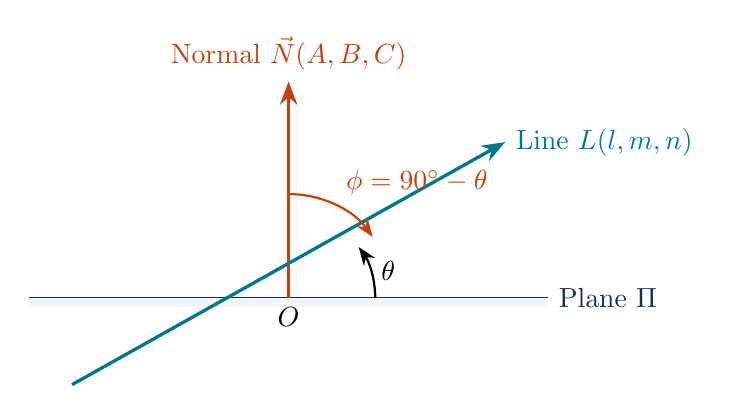
\begin{tikzpicture}[scale=1.1, >=Stealth]
    % Plane
    \draw[thick, primary] (-3,0) -- (3,0) node[right] {Plane $\Pi$};
    \fill[primary!5] (-3,-0.1) rectangle (3,0);

    % Normal
    \draw[->, very thick, accent] (0,0) -- (0,2.5) node[above] {Normal $\vec{N}(A,B,C)$};

    % Line L
    \draw[->, very thick, secondary] (-2.5,-1) -- (2.5,1.8) node[right] {Line $L(l,m,n)$};

    % Angles
    \draw[->, thick] (1,0) arc (0:36:1) node[midway, right] {$\theta$};
    \draw[->, thick, accent] (0,1.2) arc (90:36:1.2) node[midway, above right] {$\phi = 90^\circ - \theta$};

    \node[below] at (0,0) {$O$};
\end{tikzpicture}
\end{center}

Applying the cosine formula between two directed vectors (Page 22):
\begin{equation}
    \cos\phi = \frac{Al + Bm + Cn}{\sqrt{A^2 + B^2 + C^2}\,\sqrt{l^2 + m^2 + n^2}}.
\end{equation}
Since $\cos\phi = \cos(90^\circ - \theta) = \sin\theta$:
\begin{equation}
    \boxed{\sin\theta = \frac{Al + Bm + Cn}{\sqrt{A^2 + B^2 + C^2}\,\sqrt{l^2 + m^2 + n^2}}}
\end{equation}
\end{proof}

\subsection{Conditions of Parallelism and Perpendicularity}
\begin{itemize}
    \item \textbf{Line Parallel to Plane}: The line is parallel to the plane when $\theta = 0 \iff \sin\theta = 0$:
    \begin{equation}
        \boxed{Al + Bm + Cn = 0}
    \end{equation}
    (The line is perpendicular to the normal).
    \item \textbf{Line Perpendicular to Plane}: The line is perpendicular to the plane when $\theta = 90^\circ \iff \phi = 0$:
    \begin{equation}
        \boxed{\frac{A}{l} = \frac{B}{m} = \frac{C}{n}}
    \end{equation}
    (The line is parallel to the normal).
\end{itemize}

% =========================================================================
% PAGE 41
% =========================================================================
\section{Page 41: Intersection of a Line and a Plane, Foot of Perpendicular, and Image}
\label{sec:page41}

\begin{conceptbox}[Manuscript Overview: Page 41]
Page 41 solves for:
\begin{enumerate}[noitemsep]
    \item The point of intersection between a straight line and a plane.
    \item The foot of the perpendicular dropped from an external point to a plane.
    \item The optical image (reflection) of a point in a plane.
\end{enumerate}
\end{conceptbox}

\subsection{Point of Intersection of a Line and a Plane}
Let the line be $L: \frac{x - x_1}{l} = \frac{y - y_1}{m} = \frac{z - z_1}{n} = r$, and let the plane be $\Pi: Ax + By + Cz + D = 0$.
The general point on the line is $P(r) = (x_1 + lr, \; y_1 + mr, \; z_1 + nr)$.
Substitute $P(r)$ into the plane equation:
\begin{align}
    A(x_1 + lr) + B(y_1 + mr) + C(z_1 + nr) + D &= 0 \nonumber\\
    (Ax_1 + By_1 + Cz_1 + D) + r(Al + Bm + Cn) &= 0 \nonumber\\
    \implies r &= -\frac{Ax_1 + By_1 + Cz_1 + D}{Al + Bm + Cn}.
\end{align}
Substituting this value of $r$ back into $P(r)$ yields the unique point of intersection (provided $Al + Bm + Cn \neq 0$).

\subsection{Foot of Perpendicular and Image of a Point}
\begin{theorembox}[Foot of Perpendicular and Reflection Formula]
Let $P(x_0, y_0, z_0)$ be a point and $\Pi: Ax + By + Cz + D = 0$ be a plane.
\begin{enumerate}
    \item The foot of the perpendicular $N(x, y, z)$ from $P$ to $\Pi$ is given by:
    \begin{equation}
        \boxed{\frac{x - x_0}{A} = \frac{y - y_0}{B} = \frac{z - z_0}{C} = -\frac{Ax_0 + By_0 + Cz_0 + D}{A^2 + B^2 + C^2}}
    \end{equation}
    \item The image (reflection) $P'(x', y', z')$ of $P$ in the plane $\Pi$ is given by:
    \begin{equation}
        \boxed{\frac{x' - x_0}{A} = \frac{y' - y_0}{B} = \frac{z' - z_0}{C} = -2\,\frac{Ax_0 + By_0 + Cz_0 + D}{A^2 + B^2 + C^2}}
    \end{equation}
\end{enumerate}
\end{theorembox}

\begin{proof}
The normal line passing through $P(x_0, y_0, z_0)$ has direction ratios $(A, B, C)$. Its equations are:
\begin{equation}
    \frac{x - x_0}{A} = \frac{y - y_0}{B} = \frac{z - z_0}{C} = k.
\end{equation}
Any point on this normal line is $(x_0 + Ak, \; y_0 + Bk, \; z_0 + Ck)$.
For the foot of the perpendicular $N$, this point lies on the plane:
\begin{align}
    A(x_0 + Ak) + B(y_0 + Bk) + C(z_0 + Ck) + D &= 0 \nonumber\\
    (A^2 + B^2 + C^2)k + (Ax_0 + By_0 + Cz_0 + D) &= 0 \nonumber\\
    \implies k &= -\frac{Ax_0 + By_0 + Cz_0 + D}{A^2 + B^2 + C^2}.
\end{align}
For the image point $P'$, the foot $N$ is the midpoint of $PP'$:
\begin{equation}
    N = \frac{P + P'}{2} \implies P' = 2N - P.
\end{equation}
Thus, the parameter value for $P'$ is simply $2k$.
\end{proof}

% =========================================================================
% PAGE 42
% =========================================================================
\section{Page 42: Condition of Coplanarity of Two Straight Lines}
\label{sec:page42}

\begin{conceptbox}[Manuscript Overview: Page 42]
Page 42 derives the celebrated determinant condition for two lines in space to lie in the same plane (to be coplanar) and establishes the equation of the plane containing them.
\end{conceptbox}

\subsection{Derivation of the Coplanarity Condition}
\begin{theorembox}[Coplanarity Determinant Condition]
Two straight lines:
\begin{align}
    L_1 &: \frac{x - x_1}{l_1} = \frac{y - y_1}{m_1} = \frac{z - z_1}{n_1}, \label{eq:p42_L1} \\
    L_2 &: \frac{x - x_2}{l_2} = \frac{y - y_2}{m_2} = \frac{z - z_2}{n_2}, \label{eq:p42_L2}
\end{align}
are \textbf{coplanar} if and only if:
\begin{equation}
    \boxed{\begin{vmatrix}
    x_2 - x_1 & y_2 - y_1 & z_2 - z_1 \\
    l_1 & m_1 & n_1 \\
    l_2 & m_2 & n_2
    \end{vmatrix} = 0}
\end{equation}
\end{theorembox}

\begin{proof}
Any plane passing through the line $L_1$ must pass through the point $(x_1, y_1, z_1)$ and have its normal $\vec{N}(A, B, C)$ perpendicular to $L_1$:
\begin{align}
    A(x - x_1) + B(y - y_1) + C(z - z_1) &= 0, \label{eq:p42_plane} \\
    Al_1 + Bm_1 + Cn_1 &= 0. \label{eq:p42_orth1}
\end{align}
If this plane also contains the line $L_2$:
\begin{enumerate}
    \item The point $(x_2, y_2, z_2)$ on $L_2$ must lie on the plane:
    \begin{equation}
        A(x_2 - x_1) + B(y_2 - y_1) + C(z_2 - z_1) = 0. \label{eq:p42_pt2}
    \end{equation}
    \item The normal $\vec{N}(A, B, C)$ must be perpendicular to $L_2$:
    \begin{equation}
        Al_2 + Bm_2 + Cn_2 = 0. \label{eq:p42_orth2}
    \end{equation}
\end{enumerate}
Equations \eqref{eq:p42_pt2}, \eqref{eq:p42_orth1}, and \eqref{eq:p42_orth2} form a homogeneous linear system in $A, B, C$:
\begin{equation}
    \begin{pmatrix}
    x_2 - x_1 & y_2 - y_1 & z_2 - z_1 \\
    l_1 & m_1 & n_1 \\
    l_2 & m_2 & n_2
    \end{pmatrix}
    \begin{pmatrix} A \\ B \\ C \end{pmatrix} = \begin{pmatrix} 0 \\ 0 \\ 0 \end{pmatrix}.
\end{equation}
For a non-trivial plane to exist, $(A, B, C) \neq (0, 0, 0)$, so the determinant of coefficients must vanish:
\begin{equation}
    \begin{vmatrix}
    x_2 - x_1 & y_2 - y_1 & z_2 - z_1 \\
    l_1 & m_1 & n_1 \\
    l_2 & m_2 & n_2
    \end{vmatrix} = 0.
\end{equation}
\end{proof}

\subsection{Equation of the Plane Containing Two Coplanar Lines}
Eliminating $A, B, C$ between equations \eqref{eq:p42_plane}, \eqref{eq:p42_orth1}, and \eqref{eq:p42_orth2}:
\begin{equation}
    \boxed{\begin{vmatrix}
    x - x_1 & y - y_1 & z - z_1 \\
    l_1 & m_1 & n_1 \\
    l_2 & m_2 & n_2
    \end{vmatrix} = 0}
\end{equation}

% =========================================================================
% PAGE 43
% =========================================================================
\section{Page 43: Condition for a Line to Lie Wholly in a Plane}
\label{sec:page43}

\begin{conceptbox}[Manuscript Overview: Page 43]
Page 43 analyzes the algebraic conditions ensuring that a given straight line lies completely within a specified plane.
\end{conceptbox}

\begin{theorembox}[Line Lying Wholly in a Plane]
The straight line:
\begin{equation}
    L: \frac{x - x_1}{l} = \frac{y - y_1}{m} = \frac{z - z_1}{n}
\end{equation}
lies wholly and completely in the plane:
\begin{equation}
    \Pi: Ax + By + Cz + D = 0
\end{equation}
if and only if the following two conditions are simultaneously satisfied:
\begin{align}
    \text{Condition 1} &: \quad \boxed{Ax_1 + By_1 + Cz_1 + D = 0} \quad \text{(Point lies in plane)}, \\
    \text{Condition 2} &: \quad \boxed{Al + Bm + Cn = 0} \quad \text{(Line perpendicular to normal)}.
\end{align}
\end{theorembox}

\begin{proof}
Any point on line $L$ has coordinates $(x_1 + lr, \; y_1 + mr, \; z_1 + nr)$, where $r \in \mathbb{R}$.
For the line to lie entirely in the plane, this point must satisfy the equation of the plane for \emph{every} value of $r$:
\begin{align}
    A(x_1 + lr) + B(y_1 + mr) + C(z_1 + nr) + D &\equiv 0 \nonumber\\
    (Ax_1 + By_1 + Cz_1 + D) + r(Al + Bm + Cn) &\equiv 0 \quad \forall r \in \mathbb{R}.
\end{align}
A linear polynomial in $r$ is identically zero if and only if both its constant term and the coefficient of $r$ vanish independently:
\begin{align}
    Ax_1 + By_1 + Cz_1 + D &= 0, \\
    Al + Bm + Cn &= 0.
\end{align}
\end{proof}

% =========================================================================
% PAGE 44
% =========================================================================
\section{Page 44: Plane Containing a Given Line and Parallel to Another Line}
\label{sec:page44}

\begin{conceptbox}[Manuscript Overview: Page 44]
Page 44 establishes the construction of a plane that contains a given straight line and is oriented parallel to a second straight line in space.
\end{conceptbox}

\subsection{Construction and Derivation}
Let the two lines be:
\begin{align}
    L_1 &: \frac{x - x_1}{l_1} = \frac{y - y_1}{m_1} = \frac{z - z_1}{n_1}, \\
    L_2 &: \frac{x - x_2}{l_2} = \frac{y - y_2}{m_2} = \frac{z - z_2}{n_2}.
\end{align}
We seek the plane $\Pi$ containing $L_1$ and parallel to $L_2$.
\begin{enumerate}
    \item Any plane containing $L_1$ passes through $(x_1, y_1, z_1)$:
    \begin{equation}
        A(x - x_1) + B(y - y_1) + C(z - z_1) = 0 \label{eq:p44_pl}
    \end{equation}
    and its normal $\vec{N}(A, B, C)$ is perpendicular to $L_1$:
    \begin{equation}
        Al_1 + Bm_1 + Cn_1 = 0. \label{eq:p44_c1}
    \end{equation}
    \item Since the plane is parallel to $L_2$, its normal $\vec{N}$ is also perpendicular to $L_2$:
    \begin{equation}
        Al_2 + Bm_2 + Cn_2 = 0. \label{eq:p44_c2}
    \end{equation}
\end{enumerate}
Eliminating $A, B, C$ between equations \eqref{eq:p44_pl}, \eqref{eq:p44_c1}, and \eqref{eq:p44_c2}:
\begin{equation}
    \boxed{\begin{vmatrix}
    x - x_1 & y - y_1 & z - z_1 \\
    l_1 & m_1 & n_1 \\
    l_2 & m_2 & n_2
    \end{vmatrix} = 0}
\end{equation}

% =========================================================================
% PAGE 45
% =========================================================================
\section{Page 45: Line Intersecting Two Given Lines and Satisfying a Geometric Condition}
\label{sec:page45}

\begin{conceptbox}[Manuscript Overview: Page 45]
Page 45 details the method of finding a transversal line that intersects two given skew lines and either passes through a fixed point or is parallel to a given direction.
\end{conceptbox}

\subsection{Transversal Passing Through a Given Point}
Let the two given skew lines be $L_1$ and $L_2$, and let the fixed point be $P(\alpha, \beta, \gamma)$.
\begin{enumerate}
    \item \textbf{Plane 1 ($\Pi_1$)}: Determine the plane containing $L_1$ and the point $P$.
    \item \textbf{Plane 2 ($\Pi_2$)}: Determine the plane containing $L_2$ and the point $P$.
    \item \textbf{Line of Intersection}: The required transversal line is the line of intersection of planes $\Pi_1$ and $\Pi_2$:
    \begin{equation}
        \Pi_1 = 0 = \Pi_2.
    \end{equation}
    Since this line lies in $\Pi_1$, it intersects $L_1$. Since it lies in $\Pi_2$, it intersects $L_2$. Since both planes pass through $P$, the line passes through $P$.
\end{enumerate}

\subsection{Transversal Parallel to a Given Line}
If the line must be parallel to a given direction $(l, m, n)$:
\begin{enumerate}
    \item Find plane $\Pi_1$ containing $L_1$ and parallel to direction $(l, m, n)$.
    \item Find plane $\Pi_2$ containing $L_2$ and parallel to direction $(l, m, n)$.
    \item The line of intersection $\Pi_1 = 0 = \Pi_2$ is the required line.
\end{enumerate}

% =========================================================================
% PAGE 46
% =========================================================================
\section{Page 46: Skew Lines and the Concept of Shortest Distance}
\label{sec:page46}

\begin{conceptbox}[Manuscript Overview: Page 46]
Page 46 introduces \textbf{skew lines}, establishes that there exists a unique common perpendicular between them, and defines the \textbf{Shortest Distance} (S.D.).
\end{conceptbox}

\subsection{Definition of Skew Lines}
\begin{conceptbox}[Skew Lines]
Two straight lines in three-dimensional space which are neither parallel nor intersecting are called \textbf{skew lines} (or non-coplanar lines).
\end{conceptbox}

\subsection{The Common Perpendicular}
\begin{theorembox}[Existence and Uniqueness of the Common Perpendicular]
For any two non-parallel, non-intersecting lines $L_1$ and $L_2$ in space, there exists a unique straight line segment $GH$ which intersects both lines perpendicularly. The length of this segment $GH$ is the \textbf{shortest distance} between $L_1$ and $L_2$.
\end{theorembox}

\begin{center}
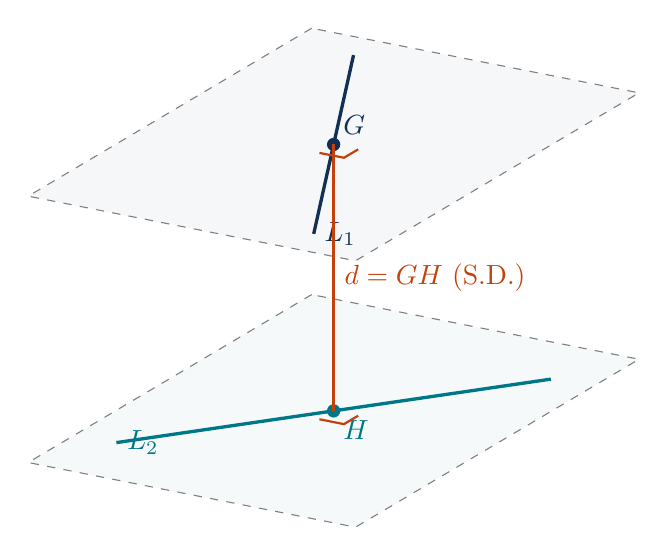
\begin{tikzpicture}[scale=1.2, >=Stealth, 3d view={120}{20}]
    % Two parallel planes enclosing skew lines
    \fill[primary!5, opacity=0.8] (-3,-2,2) -- (3,-2,2) -- (3,2,2) -- (-3,2,2) -- cycle;
    \fill[secondary!5, opacity=0.8] (-3,-2,-1) -- (3,-2,-1) -- (3,2,-1) -- (-3,2,-1) -- cycle;

    \draw[dashed, gray] (-3,-2,2) -- (3,-2,2) -- (3,2,2) -- (-3,2,2) -- cycle;
    \draw[dashed, gray] (-3,-2,-1) -- (3,-2,-1) -- (3,2,-1) -- (-3,2,-1) -- cycle;

    % Line L1 in top plane
    \draw[very thick, primary] (-2.5, -1.2, 2) -- (2.5, 1.2, 2) node[right] {$L_1$};
    \coordinate (G) at (0,0,2);
    \fill[primary] (G) circle (2pt) node[above right] {$G$};

    % Line L2 in bottom plane
    \draw[very thick, secondary] (-2, 1.5, -1) -- (2, -1.5, -1) node[right] {$L_2$};
    \coordinate (H) at (0,0,-1);
    \fill[secondary] (H) circle (2pt) node[below right] {$H$};

    % Common perpendicular GH
    \draw[very thick, accent] (H) -- (G) node[midway, right] {$d = GH \text{ (S.D.)}$};

    % Right angle markers
    \draw[thick, accent] (0,0.3,2) -- (0.3,0.3,2) -- (0.3,0,2);
    \draw[thick, accent] (0,0.3,-1) -- (0.3,0.3,-1) -- (0.3,0,-1);
\end{tikzpicture}
\end{center}

% =========================================================================
% PAGE 47
% =========================================================================
\section{Page 47: Geometric Configuration and Direction of the Common Perpendicular}
\label{sec:page47}

\begin{conceptbox}[Manuscript Overview: Page 47]
Page 47 derives the direction cosines $(\lambda, \mu, \nu)$ of the common perpendicular to two skew lines.
\end{conceptbox}

\subsection{Direction Cosines of the Common Perpendicular}
Let the two skew lines be:
\begin{align}
    L_1 &: \frac{x - x_1}{l_1} = \frac{y - y_1}{m_1} = \frac{z - z_1}{n_1}, \\
    L_2 &: \frac{x - x_2}{l_2} = \frac{y - y_2}{m_2} = \frac{z - z_2}{n_2}.
\end{align}
Let $(\lambda, \mu, \nu)$ be the direction cosines of the line of shortest distance $GH$.
Since $GH \perp L_1$ and $GH \perp L_2$:
\begin{align}
    \lambda l_1 + \mu m_1 + \nu n_1 &= 0, \label{eq:p47_gh1} \\
    \lambda l_2 + \mu m_2 + \nu n_2 &= 0. \label{eq:p47_gh2}
\end{align}
By the method of cross-multiplication:
\begin{equation}
    \frac{\lambda}{m_1 n_2 - m_2 n_1} = \frac{\mu}{n_1 l_2 - n_2 l_1} = \frac{\nu}{l_1 m_2 - l_2 m_1} = k.
\end{equation}
Since $\lambda^2 + \mu^2 + \nu^2 = 1$:
\begin{equation}
    k = \frac{1}{\sqrt{(m_1 n_2 - m_2 n_1)^2 + (n_1 l_2 - n_2 l_1)^2 + (l_1 m_2 - l_2 m_1)^2}} = \frac{1}{\sin\theta}
\end{equation}
where $\theta$ is the angle between $L_1$ and $L_2$ (Page 23).
Thus:
\begin{equation}
    \boxed{\lambda = \frac{m_1 n_2 - m_2 n_1}{\sin\theta}, \quad \mu = \frac{n_1 l_2 - n_2 l_1}{\sin\theta}, \quad \nu = \frac{l_1 m_2 - l_2 m_1}{\sin\theta}}
\end{equation}

% =========================================================================
% PAGE 48
% =========================================================================
\section{Page 48: Analytical Derivation of the Magnitude of Shortest Distance}
\label{sec:page48}

\begin{conceptbox}[Manuscript Overview: Page 48]
Page 48 delivers the complete analytical derivation of the formula for the magnitude of the shortest distance between two skew lines.
\end{conceptbox}

\begin{theorembox}[Magnitude of Shortest Distance (S.D.)]
The shortest distance $d$ between the skew lines $L_1$ and $L_2$ is:
\begin{equation}
    \boxed{d = \frac{\left|\begin{matrix}
    x_2 - x_1 & y_2 - y_1 & z_2 - z_1 \\
    l_1 & m_1 & n_1 \\
    l_2 & m_2 & n_2
    \end{matrix}\right|}{\sqrt{(m_1 n_2 - m_2 n_1)^2 + (n_1 l_2 - n_2 l_1)^2 + (l_1 m_2 - l_2 m_1)^2}}}
\end{equation}
\end{theorembox}

\begin{proof}
Let $P(x_1, y_1, z_1)$ be a point on $L_1$ and $Q(x_2, y_2, z_2)$ be a point on $L_2$.
The common perpendicular segment $GH$ is perpendicular to both lines.
Hence, the length $d = GH$ is equal to the orthogonal projection of the displacement segment $PQ$ onto the directed line $GH$ whose direction cosines are $(\lambda, \mu, \nu)$ (Page 20):
\begin{equation}
    d = |\text{Proj}_{GH}(\vec{PQ})| = |\lambda(x_2 - x_1) + \mu(y_2 - y_1) + \nu(z_2 - z_1)|.
\end{equation}
Substituting the expressions for $\lambda, \mu, \nu$ from Page 47:
\begin{align}
    d &= \left| (x_2 - x_1)\frac{m_1 n_2 - m_2 n_1}{\sin\theta} + (y_2 - y_1)\frac{n_1 l_2 - n_2 l_1}{\sin\theta} + (z_2 - z_1)\frac{l_1 m_2 - l_2 m_1}{\sin\theta} \right| \nonumber\\
    &= \frac{1}{\sin\theta} \left| (x_2 - x_1)(m_1 n_2 - m_2 n_1) + (y_2 - y_1)(n_1 l_2 - n_2 l_1) + (z_2 - z_1)(l_1 m_2 - l_2 m_1) \right|.
\end{align}
Recognizing the numerator as the expansion of a $3 \times 3$ determinant:
\begin{equation}
    d = \frac{\left|\begin{matrix}
    x_2 - x_1 & y_2 - y_1 & z_2 - z_1 \\
    l_1 & m_1 & n_1 \\
    l_2 & m_2 & n_2
    \end{matrix}\right|}{\sqrt{(m_1 n_2 - m_2 n_1)^2 + (n_1 l_2 - n_2 l_1)^2 + (l_1 m_2 - l_2 m_1)^2}}.
\end{equation}
\end{proof}

\begin{notebox}[Intersection as a Degenerate Case ($d = 0$)]
If the two lines intersect, the shortest distance between them is zero:
\begin{equation}
    d = 0 \iff \begin{vmatrix}
    x_2 - x_1 & y_2 - y_1 & z_2 - z_1 \\
    l_1 & m_1 & n_1 \\
    l_2 & m_2 & n_2
    \end{vmatrix} = 0.
\end{equation}
This perfectly reproduces the coplanarity condition established on Page 42!
\end{notebox}

% =========================================================================
% PAGE 49
% =========================================================================
\section{Page 49: Equations of the Line of Shortest Distance}
\label{sec:page49}

\begin{conceptbox}[Manuscript Overview: Page 49]
Page 49 constructs the equations of the actual straight line containing the common perpendicular $GH$, expressed as the intersection of two planes.
\end{conceptbox}

\begin{theorembox}[Equations of the Line of Shortest Distance]
The line of shortest distance between $L_1$ and $L_2$ is represented by the pair of planes:
\begin{equation}
    \boxed{\begin{vmatrix}
    x - x_1 & y - y_1 & z - z_1 \\
    l_1 & m_1 & n_1 \\
    \lambda & \mu & \nu
    \end{vmatrix} = 0 \quad \text{and} \quad
    \begin{vmatrix}
    x - x_2 & y - y_2 & z - z_2 \\
    l_2 & m_2 & n_2 \\
    \lambda & \mu & \nu
    \end{vmatrix} = 0}
\end{equation}
where $(\lambda, \mu, \nu)$ are the direction ratios of the common perpendicular.
\end{theorembox}

\begin{proof}
The line of shortest distance $GH$ intersects $L_1$ at $G$ and is perpendicular to $L_1$.
Thus, $GH$ and $L_1$ are coplanar lines intersecting at $G$.
The plane containing both $L_1$ and $GH$ passes through $(x_1, y_1, z_1)$ and has directions $(l_1, m_1, n_1)$ and $(\lambda, \mu, \nu)$. Its equation is:
\begin{equation}
    \Pi_1: \begin{vmatrix}
    x - x_1 & y - y_1 & z - z_1 \\
    l_1 & m_1 & n_1 \\
    \lambda & \mu & \nu
    \end{vmatrix} = 0.
\end{equation}
Similarly, $GH$ intersects $L_2$ at $H$ and is perpendicular to $L_2$.
The plane containing both $L_2$ and $GH$ passes through $(x_2, y_2, z_2)$ and has directions $(l_2, m_2, n_2)$ and $(\lambda, \mu, \nu)$. Its equation is:
\begin{equation}
    \Pi_2: \begin{vmatrix}
    x - x_2 & y - y_2 & z - z_2 \\
    l_2 & m_2 & n_2 \\
    \lambda & \mu & \nu
    \end{vmatrix} = 0.
\end{equation}
Since the line $GH$ lies in both planes $\Pi_1$ and $\Pi_2$, it is precisely their line of intersection $\Pi_1 = 0 = \Pi_2$.
\end{proof}

% =========================================================================
% PAGE 50
% =========================================================================
\section{Page 50: Comprehensive Solved Examination Problem on Skew Lines}
\label{sec:page50}

\begin{conceptbox}[Manuscript Overview: Page 50]
Page 50 works through an extensive university examination problem, calculating the shortest distance between two given skew lines.
\end{conceptbox}

\begin{examplebox}[Examination Problem: Shortest Distance Calculation]
Find the magnitude of the shortest distance between the lines:
\begin{align}
    L_1 &: \frac{x - 3}{3} = \frac{y - 8}{-1} = \frac{z - 3}{1}, \label{eq:ex_L1} \\
    L_2 &: \frac{x + 3}{-3} = \frac{y + 7}{2} = \frac{z - 6}{4}. \label{eq:ex_L2}
\end{align}
\end{examplebox}

\begin{proof}[Step-by-Step Analytical Solution]
\textbf{Step 1: Identify Points and Direction Ratios}:
\begin{align}
    \text{From } L_1 &: \quad P_1 = (3, 8, 3), \quad (l_1, m_1, n_1) = (3, -1, 1), \\
    \text{From } L_2 &: \quad P_2 = (-3, -7, 6), \quad (l_2, m_2, n_2) = (-3, 2, 4).
\end{align}

\textbf{Step 2: Direction Ratios of the Common Perpendicular}:
Let the common perpendicular have direction ratios $(\lambda, \mu, \nu)$:
\begin{align}
    3\lambda - \mu + \nu &= 0, \\
    -3\lambda + 2\mu + 4\nu &= 0.
\end{align}
Applying the cross-multiplication rule:
\begin{align}
    \frac{\lambda}{(-1)(4) - (1)(2)} &= \frac{\mu}{(1)(-3) - (3)(4)} = \frac{\nu}{(3)(2) - (-1)(-3)} \nonumber\\
    \frac{\lambda}{-4 - 2} &= \frac{\mu}{-3 - 12} = \frac{\nu}{6 - 3} \nonumber\\
    \frac{\lambda}{-6} &= \frac{\mu}{-15} = \frac{\nu}{3}.
\end{align}
Dividing by $-3$:
\begin{equation}
    \boxed{\frac{\lambda}{2} = \frac{\mu}{5} = \frac{\nu}{-1}}
\end{equation}
Thus, a set of direction ratios for the common perpendicular is $(a, b, c) = (2, 5, -1)$.

\textbf{Step 3: Normalize to Direction Cosines}:
\begin{align}
    \sqrt{a^2 + b^2 + c^2} &= \sqrt{2^2 + 5^2 + (-1)^2} = \sqrt{4 + 25 + 1} = \sqrt{30}. \\
    (\lambda, \mu, \nu) &= \left(\frac{2}{\sqrt{30}}, \; \frac{5}{\sqrt{30}}, \; \frac{-1}{\sqrt{30}}\right).
\end{align}

\textbf{Step 4: Vector Connecting Fixed Points}:
\begin{equation}
    \vec{P_1 P_2} = (-3 - 3)\,\hat{i} + (-7 - 8)\,\hat{j} + (6 - 3)\,\hat{k} = -6\,\hat{i} - 15\,\hat{j} + 3\,\hat{k}.
\end{equation}

\textbf{Step 5: Compute the Shortest Distance}:
\begin{align}
    d &= |\lambda(x_2 - x_1) + \mu(y_2 - y_1) + \nu(z_2 - z_1)| \nonumber\\
    &= \left| \frac{2}{\sqrt{30}}(-6) + \frac{5}{\sqrt{30}}(-15) + \frac{-1}{\sqrt{30}}(3) \right| \nonumber\\
    &= \frac{|-12 - 75 - 3|}{\sqrt{30}} = \frac{|-90|}{\sqrt{30}} = \frac{90}{\sqrt{30}}.
\end{align}
Rationalizing the denominator:
\begin{equation}
    \boxed{d = \frac{90\sqrt{30}}{30} = 3\sqrt{30}}
\end{equation}
\end{proof}

% =========================================================================
% PAGE 51
% =========================================================================
\section{Page 51: Equations of the Line of S.D. and Feet of Common Perpendicular}
\label{sec:page51}

\begin{conceptbox}[Manuscript Overview: Page 51]
Page 51 completes the examination problem by:
\begin{enumerate}[noitemsep]
    \item Finding the Cartesian equations of the line of shortest distance.
    \item Determining the exact spatial coordinates of the points of intersection (feet) $G$ and $H$.
\end{enumerate}
\end{conceptbox}

\subsection{Equations of the Line of Shortest Distance}
Applying the two-plane representation from Page 49 with $(\lambda, \mu, \nu) \sim (2, 5, -1)$:
\begin{enumerate}
    \item \textbf{Plane 1 (Containing $L_1$ and $GH$)}:
    \begin{equation}
        \begin{vmatrix}
        x - 3 & y - 8 & z - 3 \\
        3 & -1 & 1 \\
        2 & 5 & -1
        \end{vmatrix} = 0.
    \end{equation}
    Expanding along row 1:
    \begin{align}
        (x - 3)[(-1)(-1) - (1)(5)] - (y - 8)[(3)(-1) - (1)(2)] + (z - 3)[(3)(5) - (-1)(2)] &= 0 \nonumber\\
        (x - 3)(1 - 5) - (y - 8)(-3 - 2) + (z - 3)(15 + 2) &= 0 \nonumber\\
        -4(x - 3) + 5(y - 8) + 17(z - 3) &= 0 \nonumber\\
        -4x + 12 + 5y - 40 + 17z - 51 &= 0 \nonumber\\
        \Aboxed{4x - 5y - 17z + 79 &= 0} \label{eq:p51_pl1}
    \end{align}
    \item \textbf{Plane 2 (Containing $L_2$ and $GH$)}:
    \begin{equation}
        \begin{vmatrix}
        x + 3 & y + 7 & z - 6 \\
        -3 & 2 & 4 \\
        2 & 5 & -1
        \end{vmatrix} = 0.
    \end{equation}
    Expanding along row 1:
    \begin{align}
        (x + 3)[(2)(-1) - (4)(5)] - (y + 7)[(-3)(-1) - (4)(2)] + (z - 6)[(-3)(5) - (2)(2)] &= 0 \nonumber\\
        (x + 3)(-2 - 20) - (y + 7)(3 - 8) + (z - 6)(-15 - 4) &= 0 \nonumber\\
        -22(x + 3) + 5(y + 7) - 19(z - 6) &= 0 \nonumber\\
        -22x - 66 + 5y + 35 - 19z + 114 &= 0 \nonumber\\
        \Aboxed{22x - 5y + 19z - 83 &= 0} \label{eq:p51_pl2}
    \end{align}
\end{enumerate}
The equations of the line of shortest distance are given by \eqref{eq:p51_pl1} and \eqref{eq:p51_pl2} simultaneously.

\subsection{Coordinates of the Feet $G$ and $H$}
Let $G$ be a point on $L_1$ and $H$ be a point on $L_2$:
\begin{align}
    G &= (3 + 3r, \; 8 - r, \; 3 + r), \\
    H &= (-3 - 3s, \; -7 + 2s, \; 6 + 4s).
\end{align}
The direction ratios of the segment $GH$ are:
\begin{equation}
    \vec{GH} = H - G = \bigl(-6 - 3s - 3r, \; -15 + 2s + r, \; 3 + 4s - r\bigr).
\end{equation}
Since $GH$ is along the common perpendicular with DRs $(2, 5, -1)$:
\begin{equation}
    \frac{-6 - 3s - 3r}{2} = \frac{-15 + 2s + r}{5} = \frac{3 + 4s - r}{-1} = k.
\end{equation}
Solving this linear system yields $r = 0$ and $s = 0$!
Hence:
\begin{equation}
    \boxed{G = (3, 8, 3), \quad H = (-3, -7, 6)}
\end{equation}
\textbf{Verification}:
\begin{equation}
    GH = \sqrt{(-3-3)^2 + (-7-8)^2 + (6-3)^2} = \sqrt{(-6)^2 + (-15)^2 + 3^2} = \sqrt{36 + 225 + 9} = \sqrt{270} = 3\sqrt{30}.
\end{equation}
The distance matches the formula from Page 50 precisely!

% =========================================================================
% PAGE 52
% =========================================================================
\section{Page 52: Distance Between Parallel Lines and Chapter Summary}
\label{sec:page52}

\begin{conceptbox}[Manuscript Overview: Page 52]
Page 52 concludes the analytical treatment of lines by considering the case of \textbf{parallel lines} (where $\vec{b}_1 \times \vec{b}_2 = \vec{0}$) and provides a comparative summary.
\end{conceptbox}

\subsection{Shortest Distance Between Parallel Lines}
If two lines $L_1$ and $L_2$ are parallel, their direction ratios are proportional:
\begin{align}
    L_1 &: \frac{x - x_1}{l} = \frac{y - y_1}{m} = \frac{z - z_1}{n}, \\
    L_2 &: \frac{x - x_2}{l} = \frac{y - y_2}{m} = \frac{z - z_2}{n}.
\end{align}
Here, the lines lie in a common plane, and the cross product of their directions vanishes.
The perpendicular distance $d$ between them is obtained by taking the projection of $\vec{P_1 P_2}$ perpendicular to the direction vector $\hat{u}(l, m, n)$:

\begin{theorembox}[Distance Between Parallel Lines]
The perpendicular distance between two parallel lines with unit direction vector $\hat{u} = l\,\hat{i} + m\,\hat{j} + n\,\hat{k}$ is:
\begin{equation}
    \boxed{d = |\vec{P_1 P_2} \times \hat{u}| = \frac{\sqrt{\begin{vmatrix} y_2-y_1 & z_2-z_1 \\ m & n \end{vmatrix}^2 + \begin{vmatrix} z_2-z_1 & x_2-x_1 \\ n & l \end{vmatrix}^2 + \begin{vmatrix} x_2-x_1 & y_2-y_1 \\ l & m \end{vmatrix}^2}}{\sqrt{l^2 + m^2 + n^2}}}
\end{equation}
\end{theorembox}

\subsection{Summary of Spatial Line Geometry}
\begin{center}
\begin{tabular}{|l|l|}
\hline
\textbf{Geometric Entity} & \textbf{Standard Analytical Expression} \\
\hline
Symmetrical line & $\frac{x-x_1}{l} = \frac{y-y_1}{m} = \frac{z-z_1}{n} = r$ \\
General point on line & $(x_1 + lr, \; y_1 + mr, \; z_1 + nr)$ \\
Angle with plane & $\sin\theta = \frac{Al+Bm+Cn}{\sqrt{\sum A^2}\sqrt{\sum l^2}}$ \\
Coplanarity condition & $\det[\vec{P_2}-\vec{P_1}, \; \vec{b}_1, \; \vec{b}_2] = 0$ \\
Shortest distance (skew) & $d = \frac{|\det[\vec{P_2}-\vec{P_1}, \; \vec{b}_1, \; \vec{b}_2]|}{|\vec{b}_1 \times \vec{b}_2|}$ \\
Distance (parallel) & $d = \frac{|(\vec{P_2}-\vec{P_1}) \times \vec{b}|}{|\vec{b}|}$ \\
\hline
\end{tabular}
\end{center}

\chapter{Vector Treatment of Planes and Lines (Pages 53--62)}
\label{ch:vectors}

% =========================================================================
% PAGE 53
% =========================================================================
\section{Page 53: Vector Equation of a Plane --- Normal Form and One-Point Form}
\label{sec:page53}

\begin{conceptbox}[Manuscript Overview: Page 53]
Page 53 introduces the vector algebraic formulation of three-dimensional planes. It develops the vector normal form $\vec{r} \cdot \hat{n} = p$ and the one-point vector form $(\vec{r} - \vec{a}) \cdot \vec{n} = 0$, linking them directly with Cartesian coordinates.
\end{conceptbox}

\subsection{The Vector Normal Form of a Plane}
\begin{theorembox}[Vector Normal Form]
The vector equation of a plane situated at a perpendicular distance $p$ from the origin, with unit normal vector $\hat{n}$ pointing from the origin toward the plane, is:
\begin{equation}
    \boxed{\vec{r} \cdot \hat{n} = p} \quad (p \ge 0)
\end{equation}
\end{theorembox}

\begin{proof}
Let $O$ be the origin of vectors.
Draw $ON$ perpendicular to the given plane, meeting it at $N$.
The length of $ON$ is $p \ge 0$, and the unit vector in the direction of $\vec{ON}$ is $\hat{n}$, so:
\begin{equation}
    \vec{ON} = p\,\hat{n}.
\end{equation}
Let $P$ be any arbitrary point on the plane with position vector $\vec{r} = \vec{OP}$.
Join $NP$. Since $ON$ is normal to the entire plane, it is perpendicular to every vector lying in the plane:
\begin{equation}
    \vec{NP} \perp \vec{ON} \iff \vec{NP} \cdot \vec{ON} = 0.
\end{equation}
From vector triangle $\triangle ONP$:
\begin{equation}
    \vec{NP} = \vec{OP} - \vec{ON} = \vec{r} - p\,\hat{n}.
\end{equation}
Taking the scalar product with $\hat{n}$:
\begin{align}
    (\vec{r} - p\,\hat{n}) \cdot \hat{n} &= 0 \nonumber\\
    \vec{r} \cdot \hat{n} - p(\hat{n} \cdot \hat{n}) &= 0.
\end{align}
Since $\hat{n}$ is a unit vector, $\hat{n} \cdot \hat{n} = |\hat{n}|^2 = 1$. Therefore:
\begin{equation}
    \boxed{\vec{r} \cdot \hat{n} = p}
\end{equation}
\end{proof}

\subsection{Connection with Cartesian Coordinates}
Let $\vec{r} = x\,\hat{i} + y\,\hat{j} + z\,\hat{k}$, and let $\hat{n} = l\,\hat{i} + m\,\hat{j} + n\,\hat{k}$ (where $l^2+m^2+n^2=1$).
Then:
\begin{equation}
    \vec{r} \cdot \hat{n} = (x\,\hat{i} + y\,\hat{j} + z\,\hat{k}) \cdot (l\,\hat{i} + m\,\hat{j} + n\,\hat{k}) = lx + my + nz.
\end{equation}
Substituting this into $\vec{r} \cdot \hat{n} = p$ recovers the Cartesian normal form of Page 27:
\begin{equation}
    lx + my + nz = p.
\end{equation}

\subsection{Plane Passing Through a Point with Given Normal}
\begin{theorembox}[One-Point Vector Form]
The vector equation of a plane passing through a point $A$ with position vector $\vec{a}$ and perpendicular to a non-zero normal vector $\vec{n}$ is:
\begin{equation}
    \boxed{(\vec{r} - \vec{a}) \cdot \vec{n} = 0 \iff \vec{r} \cdot \vec{n} = \vec{a} \cdot \vec{n}}
\end{equation}
\end{theorembox}

\begin{proof}
Let $P(\vec{r})$ be any point on the plane.
The displacement vector $\vec{AP} = \vec{r} - \vec{a}$ lies entirely in the plane.
Since $\vec{n}$ is normal to the plane, $\vec{AP} \perp \vec{n} \implies (\vec{r} - \vec{a}) \cdot \vec{n} = 0$.
Expanding the dot product gives $\vec{r} \cdot \vec{n} = \vec{a} \cdot \vec{n} = d$.
\end{proof}

% =========================================================================
% PAGE 54
% =========================================================================
\section{Page 54: General Vector Plane Equations and Perpendicular Distance}
\label{sec:page54}

\begin{conceptbox}[Manuscript Overview: Page 54]
Page 54 investigates the general vector equation $\vec{r} \cdot \vec{n} = d$ (where $\vec{n}$ is not necessarily a unit vector), its normalization, and the vector formula for the perpendicular distance from an arbitrary point to a plane.
\end{conceptbox}

\subsection{General Vector Equation and Normalization}
The general linear vector equation of a plane is:
\begin{equation}
    \vec{r} \cdot \vec{n} = d
\end{equation}
where $\vec{n} = A\,\hat{i} + B\,\hat{j} + C\,\hat{k}$ is any normal vector and $d$ is a scalar constant.
Dividing both sides by the magnitude $|\vec{n}| = \sqrt{A^2 + B^2 + C^2}$:
\begin{equation}
    \vec{r} \cdot \left(\frac{\vec{n}}{|\vec{n}|}\right) = \frac{d}{|\vec{n}|} \iff \vec{r} \cdot \hat{n} = p
\end{equation}
where $p = \frac{|d|}{|\vec{n}|}$ represents the true perpendicular distance from the origin.

\subsection{Perpendicular Distance of a Point from a Vector Plane}
\begin{theorembox}[Perpendicular Distance to a Plane in Vector Form]
The perpendicular distance $D$ of a point $P$ with position vector $\vec{a}$ from the plane $\vec{r} \cdot \vec{n} = d$ is:
\begin{equation}
    \boxed{D = \frac{|\vec{a} \cdot \vec{n} - d|}{|\vec{n}|}}
\end{equation}
\end{theorembox}

\begin{proof}
Let $\Pi$ be the plane $\vec{r} \cdot \vec{n} = d$, and let $N$ be the foot of the perpendicular from $P(\vec{a})$ to $\Pi$.
The displacement vector $\vec{PN}$ is parallel to the normal $\vec{n}$, so $\vec{PN} = \pm D\,\hat{n} = \pm D\,\frac{\vec{n}}{|\vec{n}|}$.
The position vector of $N$ is:
\begin{equation}
    \vec{r}_N = \vec{a} + \vec{PN} = \vec{a} \pm D\,\frac{\vec{n}}{|\vec{n}|}.
\end{equation}
Since $N$ lies on the plane $\Pi$, its position vector satisfies $\vec{r}_N \cdot \vec{n} = d$:
\begin{align}
    \left(\vec{a} \pm D\,\frac{\vec{n}}{|\vec{n}|}\right) \cdot \vec{n} &= d \nonumber\\
    \vec{a} \cdot \vec{n} \pm D\,\frac{|\vec{n}|^2}{|\vec{n}|} &= d \nonumber\\
    \vec{a} \cdot \vec{n} \pm D|\vec{n}| &= d \nonumber\\
    \pm D|\vec{n}| &= d - \vec{a} \cdot \vec{n}.
\end{align}
Taking the absolute value on both sides:
\begin{equation}
    D|\vec{n}| = |\vec{a} \cdot \vec{n} - d| \implies \boxed{D = \frac{|\vec{a} \cdot \vec{n} - d|}{|\vec{n}|}}.
\end{equation}
\end{proof}

\subsection{Distance Between Two Parallel Planes in Vector Form}
If two planes are parallel, their normals are parallel and can be taken as the same vector $\vec{n}$:
\begin{equation}
    \Pi_1: \vec{r} \cdot \vec{n} = d_1, \quad \Pi_2: \vec{r} \cdot \vec{n} = d_2.
\end{equation}
The perpendicular distance between them is:
\begin{equation}
    \boxed{D = \frac{|d_1 - d_2|}{|\vec{n}|}}
\end{equation}

% =========================================================================
% PAGE 55
% =========================================================================
\section{Page 55: Angle Between Two Planes and Plane Through Three Points}
\label{sec:page55}

\begin{conceptbox}[Manuscript Overview: Page 55]
Page 55 develops the vector formulation for:
\begin{enumerate}[noitemsep]
    \item The angle between two planes and the conditions of parallelism and perpendicularity.
    \item The vector equation of a plane passing through three non-collinear points.
\end{enumerate}
\end{conceptbox}

\subsection{Angle Between Two Planes}
\begin{theorembox}[Angle Between Two Vector Planes]
The angle $\theta$ between the two planes $\vec{r} \cdot \vec{n}_1 = d_1$ and $\vec{r} \cdot \vec{n}_2 = d_2$ is equal to the angle between their normal vectors $\vec{n}_1$ and $\vec{n}_2$:
\begin{equation}
    \boxed{\cos\theta = \frac{\vec{n}_1 \cdot \vec{n}_2}{|\vec{n}_1|\,|\vec{n}_2|}}
\end{equation}
\end{theorembox}

\begin{notebox}[Parallelism and Perpendicularity]
\begin{itemize}[noitemsep]
    \item \textbf{Perpendicular Planes} ($\theta = 90^\circ$): $\cos\theta = 0 \iff \boxed{\vec{n}_1 \cdot \vec{n}_2 = 0}$.
    \item \textbf{Parallel Planes} ($\theta = 0$ or $\pi$): $\vec{n}_1$ is parallel to $\vec{n}_2 \iff \boxed{\vec{n}_1 \times \vec{n}_2 = \vec{0}}$ or $\vec{n}_1 = \lambda \vec{n}_2$.
\end{itemize}
\end{notebox}

\subsection{Plane Passing Through Three Points in Vector Form}
\begin{theorembox}[Plane Through Three Points]
The vector equation of the plane passing through three non-collinear points with position vectors $\vec{a}, \vec{b}, \vec{c}$ is:
\begin{equation}
    \boxed{(\vec{r} - \vec{a}) \cdot \bigl[(\vec{b} - \vec{a}) \times (\vec{c} - \vec{a})\bigr] = 0 \iff [\vec{r} - \vec{a}, \; \vec{b} - \vec{a}, \; \vec{c} - \vec{a}] = 0}
\end{equation}
In expanded scalar triple product notation:
\begin{equation}
    \boxed{\vec{r} \cdot (\vec{a} \times \vec{b} + \vec{b} \times \vec{c} + \vec{c} \times \vec{a}) = [\vec{a}, \vec{b}, \vec{c}]}
\end{equation}
\end{theorembox}

\begin{proof}
Let $A(\vec{a}), B(\vec{b}), C(\vec{c})$ be the three given points in the plane, and let $P(\vec{r})$ be any point on the plane.
The vectors $\vec{AB} = \vec{b} - \vec{a}$ and $\vec{AC} = \vec{c} - \vec{a}$ both lie in the plane.
Their vector cross product:
\begin{equation}
    \vec{n} = (\vec{b} - \vec{a}) \times (\vec{c} - \vec{a})
\end{equation}
is normal to the plane.
Since the vector $\vec{AP} = \vec{r} - \vec{a}$ also lies in the plane, it is perpendicular to the normal $\vec{n}$:
\begin{equation}
    (\vec{r} - \vec{a}) \cdot \vec{n} = 0 \implies (\vec{r} - \vec{a}) \cdot \bigl[(\vec{b} - \vec{a}) \times (\vec{c} - \vec{a})\bigr] = 0.
\end{equation}
Expanding the cross product:
\begin{align}
    (\vec{b} - \vec{a}) \times (\vec{c} - \vec{a}) &= \vec{b} \times \vec{c} - \vec{b} \times \vec{a} - \vec{a} \times \vec{c} + \vec{a} \times \vec{a} \nonumber\\
    &= \vec{b} \times \vec{c} + \vec{a} \times \vec{b} + \vec{c} \times \vec{a}.
\end{align}
Taking the dot product with $\vec{r} - \vec{a}$:
\begin{align}
    \vec{r} \cdot (\vec{a} \times \vec{b} + \vec{b} \times \vec{c} + \vec{c} \times \vec{a}) &= \vec{a} \cdot (\vec{a} \times \vec{b} + \vec{b} \times \vec{c} + \vec{c} \times \vec{a}) \nonumber\\
    &= \vec{a} \cdot (\vec{a} \times \vec{b}) + \vec{a} \cdot (\vec{b} \times \vec{c}) + \vec{a} \cdot (\vec{c} \times \vec{a}).
\end{align}
Since $\vec{a} \cdot (\vec{a} \times \vec{b}) = 0$ and $\vec{a} \cdot (\vec{c} \times \vec{a}) = 0$:
\begin{equation}
    \vec{r} \cdot (\vec{a} \times \vec{b} + \vec{b} \times \vec{c} + \vec{c} \times \vec{a}) = [\vec{a}, \vec{b}, \vec{c}].
\end{equation}
\end{proof}

% =========================================================================
% PAGE 56
% =========================================================================
\section{Page 56: Vector Family of Planes Through an Intersection Line}
\label{sec:page56}

\begin{conceptbox}[Manuscript Overview: Page 56]
Page 56 derives the vector equation representing the family of planes passing through the line of intersection of two given vector planes.
\end{conceptbox}

\begin{theorembox}[Family of Planes in Vector Form]
Let two planes be given in vector form by:
\begin{align}
    \Pi_1 &: \vec{r} \cdot \vec{n}_1 = d_1, \\
    \Pi_2 &: \vec{r} \cdot \vec{n}_2 = d_2.
\end{align}
The vector equation of any plane passing through their line of intersection is:
\begin{equation}
    \boxed{(\vec{r} \cdot \vec{n}_1 - d_1) + \lambda(\vec{r} \cdot \vec{n}_2 - d_2) = 0 \iff \vec{r} \cdot (\vec{n}_1 + \lambda \vec{n}_2) = d_1 + \lambda d_2}
\end{equation}
where $\lambda$ is an arbitrary scalar parameter.
\end{theorembox}

\begin{proof}
\begin{enumerate}
    \item The equation $\vec{r} \cdot (\vec{n}_1 + \lambda \vec{n}_2) = d_1 + \lambda d_2$ is linear in $\vec{r}$, with normal vector $\vec{n} = \vec{n}_1 + \lambda \vec{n}_2$. By Page 54, it represents a plane for every value of $\lambda$.
    \item Let $\vec{r}_0$ be any point on the line of intersection of $\Pi_1$ and $\Pi_2$.
    Then $\vec{r}_0$ satisfies both equations:
    \begin{equation}
        \vec{r}_0 \cdot \vec{n}_1 = d_1 \quad \text{and} \quad \vec{r}_0 \cdot \vec{n}_2 = d_2.
    \end{equation}
    Substituting $\vec{r}_0$ into the family equation:
    \begin{equation}
        (\vec{r}_0 \cdot \vec{n}_1 - d_1) + \lambda(\vec{r}_0 \cdot \vec{n}_2 - d_2) = (d_1 - d_1) + \lambda(d_2 - d_2) = 0 + \lambda(0) = 0.
    \end{equation}
    Thus, every point of the line of intersection lies on the plane.
\end{enumerate}
\end{proof}

% =========================================================================
% PAGE 57
% =========================================================================
\section{Page 57: Vector Equations of Dihedral Angle Bisectors}
\label{sec:page57}

\begin{conceptbox}[Manuscript Overview: Page 57]
Page 57 translates the theory of dihedral angle bisectors into vector algebra, providing a coordinate-free formulation of the bisector planes.
\end{conceptbox}

\subsection{Derivation of the Vector Bisector Equations}
Let two planes be given in vector form:
\begin{align}
    \Pi_1 &: \vec{r} \cdot \vec{n}_1 = d_1, \\
    \Pi_2 &: \vec{r} \cdot \vec{n}_2 = d_2.
\end{align}
Let $\vec{r}$ be the position vector of any point lying on a bisecting plane.
By definition, its perpendicular distances from $\Pi_1$ and $\Pi_2$ must be equal:
\begin{equation}
    \frac{|\vec{r} \cdot \vec{n}_1 - d_1|}{|\vec{n}_1|} = \frac{|\vec{r} \cdot \vec{n}_2 - d_2|}{|\vec{n}_2|}.
\end{equation}
Removing the absolute value signs yields the two bisecting planes:
\begin{equation}
    \boxed{\frac{\vec{r} \cdot \vec{n}_1 - d_1}{|\vec{n}_1|} = \pm \frac{\vec{r} \cdot \vec{n}_2 - d_2|}{|\vec{n}_2|}}
\end{equation}
Rewriting in terms of unit normal vectors $\hat{n}_1 = \frac{\vec{n}_1}{|\vec{n}_1|}$ and $\hat{n}_2 = \frac{\vec{n}_2}{|\vec{n}_2|}$, with $p_1 = \frac{d_1}{|\vec{n}_1|}$ and $p_2 = \frac{d_2}{|\vec{n}_2|}$:
\begin{equation}
    \boxed{\vec{r} \cdot (\hat{n}_1 \mp \hat{n}_2) = p_1 \mp p_2}
\end{equation}

\subsection{Orthogonality of the Vector Bisectors}
The normal vectors to the two bisector planes are $\vec{N}_+ = \hat{n}_1 - \hat{n}_2$ and $\vec{N}_- = \hat{n}_1 + \hat{n}_2$.
Their scalar product is:
\begin{equation}
    \vec{N}_+ \cdot \vec{N}_- = (\hat{n}_1 - \hat{n}_2) \cdot (\hat{n}_1 + \hat{n}_2) = |\hat{n}_1|^2 - |\hat{n}_2|^2 = 1 - 1 = \mathbf{0}.
\end{equation}
This confirms that the two bisector planes are mutually orthogonal.

% =========================================================================
% PAGE 58
% =========================================================================
\section{Page 58: Vector Equation of a Straight Line}
\label{sec:page58}

\begin{conceptbox}[Manuscript Overview: Page 58]
Page 58 derives the vector equations of a straight line in space: the point-direction parametric form, the cross-product non-parametric form, and the two-point form.
\end{conceptbox}

\subsection{Point-Direction Vector Form}
\begin{theorembox}[Vector Equation of a Line]
The vector equation of a straight line passing through a point $A$ with position vector $\vec{a}$ and parallel to a non-zero vector $\vec{b}$ is:
\begin{equation}
    \boxed{\vec{r} = \vec{a} + \lambda \vec{b}, \quad \lambda \in \mathbb{R}}
\end{equation}
\end{theorembox}

\begin{proof}
Let $P$ be any point on the line with position vector $\vec{r} = \vec{OP}$.
The displacement vector $\vec{AP} = \vec{OP} - \vec{OA} = \vec{r} - \vec{a}$ lies along the line.
Since the line is parallel to vector $\vec{b}$, the vector $\vec{r} - \vec{a}$ is collinear with $\vec{b}$:
\begin{equation}
    \vec{r} - \vec{a} = \lambda \vec{b} \iff \vec{r} = \vec{a} + \lambda \vec{b}.
\end{equation}
\end{proof}

\begin{center}
\begin{tikzpicture}[scale=1.1, >=Stealth]
    \coordinate (O) at (0,0);
    \coordinate (A) at (1.5, 2.0);
    \coordinate (B) at (3.5, 1.2);

    % Line L
    \draw[very thick, primary] ($(A)-1.2*(B)$) -- ($(A)+2.2*(B)$) node[right] {Line $L$};

    % Point P on line
    \coordinate (P) at ($(A)+1.4*(B)$);

    % Vectors
    \draw[->, thick, secondary] (O) -- (A) node[midway, left] {$\vec{a}$};
    \draw[->, thick, secondary] (O) -- (P) node[midway, right] {$\vec{r}$};
    \draw[->, very thick, accent] (A) -- (P) node[midway, above left] {$\lambda\vec{b}$};

    \fill (O) circle (2pt) node[below left] {$O$};
    \fill[secondary] (A) circle (2pt) node[above left] {$A(\vec{a})$};
    \fill[accent] (P) circle (2pt) node[above right] {$P(\vec{r})$};
\end{tikzpicture}
\end{center}

\subsection{Non-Parametric Cross-Product Form}
Since $\vec{r} - \vec{a}$ is collinear with $\vec{b}$, their vector cross product must vanish:
\begin{equation}
    \boxed{(\vec{r} - \vec{a}) \times \vec{b} = \vec{0} \iff \vec{r} \times \vec{b} = \vec{a} \times \vec{b}}
\end{equation}

\subsection{Two-Point Vector Form}
If the line passes through two distinct points $A(\vec{a})$ and $B(\vec{b})$, its direction vector is $\vec{b} - \vec{a}$:
\begin{equation}
    \boxed{\vec{r} = \vec{a} + \lambda(\vec{b} - \vec{a}) = (1 - \lambda)\vec{a} + \lambda \vec{b}}
\end{equation}
In non-parametric form:
\begin{equation}
    \boxed{(\vec{r} - \vec{a}) \times (\vec{b} - \vec{a}) = \vec{0}}
\end{equation}

% =========================================================================
% PAGE 59
% =========================================================================
\section{Page 59: Perpendicular Distance of a Point from a Vector Line}
\label{sec:page59}

\begin{conceptbox}[Manuscript Overview: Page 59]
Page 59 derives the vector formula for the perpendicular distance from an external point to a straight line and determines the foot of the perpendicular.
\end{conceptbox}

\begin{theorembox}[Perpendicular Distance from Point to Line]
The perpendicular distance $d$ from a point $P$ with position vector $\vec{p}$ to the straight line $\vec{r} = \vec{a} + \lambda \vec{b}$ is:
\begin{equation}
    \boxed{d = \frac{|(\vec{p} - \vec{a}) \times \vec{b}|}{|\vec{b}|}}
\end{equation}
\end{theorembox}

\begin{proof}
Let $A$ be the point on the line with position vector $\vec{a}$, and let $N$ be the foot of the perpendicular dropped from $P(\vec{p})$ onto the line.
In the right-angled triangle $\triangle APN$, the angle at $N$ is $90^\circ$:
\begin{equation}
    d = PN = AP\sin\theta = |\vec{p} - \vec{a}|\sin\theta
\end{equation}
where $\theta$ is the angle between the vector $\vec{AP} = \vec{p} - \vec{a}$ and the line direction vector $\vec{b}$.
By the geometric definition of the vector cross product magnitude:
\begin{equation}
    |(\vec{p} - \vec{a}) \times \vec{b}| = |\vec{p} - \vec{a}|\,|\vec{b}|\sin\theta.
\end{equation}
Dividing by $|\vec{b}|$:
\begin{equation}
    d = |\vec{p} - \vec{a}|\sin\theta = \frac{|(\vec{p} - \vec{a}) \times \vec{b}|}{|\vec{b}|}.
\end{equation}
\end{proof}

\subsection{Foot of the Perpendicular in Vector Form}
The foot $N$ has position vector $\vec{n} = \vec{a} + \lambda_0 \vec{b}$.
Since $PN \perp \vec{b}$:
\begin{align}
    (\vec{n} - \vec{p}) \cdot \vec{b} &= 0 \nonumber\\
    \bigl[(\vec{a} + \lambda_0 \vec{b}) - \vec{p}\bigr] \cdot \vec{b} &= 0 \nonumber\\
    (\vec{a} - \vec{p}) \cdot \vec{b} + \lambda_0 |\vec{b}|^2 &= 0 \nonumber\\
    \implies \lambda_0 &= \frac{(\vec{p} - \vec{a}) \cdot \vec{b}}{|\vec{b}|^2}.
\end{align}
Substituting $\lambda_0$ back gives the exact position vector of the foot $N$:
\begin{equation}
    \boxed{\vec{r}_N = \vec{a} + \left( \frac{(\vec{p} - \vec{a}) \cdot \vec{b}}{|\vec{b}|^2} \right)\vec{b}}
\end{equation}

% =========================================================================
% PAGE 60
% =========================================================================
\section{Page 60: Coplanarity of Vector Lines and the Plane Containing Them}
\label{sec:page60}

\begin{conceptbox}[Manuscript Overview: Page 60]
Page 60 establishes the necessary and sufficient condition for two vector straight lines to be coplanar and derives the vector equation of the unique plane containing them.
\end{conceptbox}

\begin{theorembox}[Coplanarity of Vector Lines]
Two straight lines:
\begin{align}
    L_1 &: \vec{r} = \vec{a}_1 + \lambda \vec{b}_1, \\
    L_2 &: \vec{r} = \vec{a}_2 + \mu \vec{b}_2,
\end{align}
are \textbf{coplanar} if and only if their scalar triple product vanishes:
\begin{equation}
    \boxed{(\vec{a}_2 - \vec{a}_1) \cdot (\vec{b}_1 \times \vec{b}_2) = 0 \iff [\vec{a}_2 - \vec{a}_1, \; \vec{b}_1, \; \vec{b}_2] = 0}
\end{equation}
\end{theorembox}

\begin{proof}
Let $A_1$ and $A_2$ be the points on $L_1$ and $L_2$ with position vectors $\vec{a}_1$ and $\vec{a}_2$.
The displacement vector between them is $\vec{A_1 A_2} = \vec{a}_2 - \vec{a}_1$.
If the two lines lie in a common plane:
\begin{enumerate}
    \item The line direction vectors $\vec{b}_1$ and $\vec{b}_2$ are parallel to the plane.
    \item The displacement vector $\vec{a}_2 - \vec{a}_1$ joining points on the two lines lies entirely in the plane.
\end{enumerate}
Therefore, the three vectors $\vec{a}_2 - \vec{a}_1, \vec{b}_1, \vec{b}_2$ are coplanar.
Three vectors are coplanar if and only if the volume of the parallelepiped formed by them is zero, which is given by their scalar triple product:
\begin{equation}
    (\vec{a}_2 - \vec{a}_1) \cdot (\vec{b}_1 \times \vec{b}_2) = 0.
\end{equation}
\end{proof}

\subsection{Plane Containing the Two Coplanar Lines}
The plane containing both lines passes through $\vec{a}_1$ and has normal $\vec{n} = \vec{b}_1 \times \vec{b}_2$:
\begin{equation}
    \boxed{(\vec{r} - \vec{a}_1) \cdot (\vec{b}_1 \times \vec{b}_2) = 0}
\end{equation}

% =========================================================================
% PAGE 61
% =========================================================================
\section{Page 61: Shortest Distance Between Skew Lines in Vector Form}
\label{sec:page61}

\begin{conceptbox}[Manuscript Overview: Page 61]
Page 61 derives the vector formula for the shortest distance between two skew lines using vector projections and scalar triple products.
\end{conceptbox}

\begin{theorembox}[Shortest Distance in Vector Form]
The shortest distance $d$ between the skew lines:
\begin{align}
    L_1 &: \vec{r} = \vec{a}_1 + \lambda \vec{b}_1, \\
    L_2 &: \vec{r} = \vec{a}_2 + \mu \vec{b}_2,
\end{align}
is given by:
\begin{equation}
    \boxed{d = \frac{|(\vec{a}_2 - \vec{a}_1) \cdot (\vec{b}_1 \times \vec{b}_2)|}{|\vec{b}_1 \times \vec{b}_2|}}
\end{equation}
\end{theorembox}

\begin{proof}
The shortest distance occurs along the line segment $GH$ perpendicular to both lines $L_1$ and $L_2$.
The direction of the common perpendicular is perpendicular to both $\vec{b}_1$ and $\vec{b}_2$:
\begin{equation}
    \vec{n} = \vec{b}_1 \times \vec{b}_2.
\end{equation}
The unit vector along the common perpendicular is:
\begin{equation}
    \hat{n} = \frac{\vec{b}_1 \times \vec{b}_2}{|\vec{b}_1 \times \vec{b}_2|}.
\end{equation}
Let $A_1(\vec{a}_1)$ be on $L_1$ and $A_2(\vec{a}_2)$ be on $L_2$.
The shortest distance $d$ is the magnitude of the orthogonal projection of $\vec{A_1 A_2} = \vec{a}_2 - \vec{a}_1$ onto $\hat{n}$:
\begin{equation}
    d = |(\vec{a}_2 - \vec{a}_1) \cdot \hat{n}| = \frac{|(\vec{a}_2 - \vec{a}_1) \cdot (\vec{b}_1 \times \vec{b}_2)|}{|\vec{b}_1 \times \vec{b}_2|}.
\end{equation}
\end{proof}

\subsection{Shortest Distance Between Parallel Lines in Vector Form}
When the lines are parallel, $\vec{b}_1 = \vec{b}_2 = \vec{b}$:
\begin{equation}
    \boxed{d = \frac{|(\vec{a}_2 - \vec{a}_1) \times \vec{b}|}{|\vec{b}|}}
\end{equation}

% =========================================================================
% PAGE 62
% =========================================================================
\section{Page 62: Solved Vector Examination Problems}
\label{sec:page62}

\begin{conceptbox}[Manuscript Overview: Page 62]
Page 62 solves standard university examination problems illustrating vector shortest distance calculations and intersection algorithms.
\end{conceptbox}

\begin{examplebox}[Problem: Vector Shortest Distance Calculation]
Find the shortest distance between the two lines whose vector equations are:
\begin{align}
    L_1 &: \vec{r} = (\hat{i} + 2\hat{j} + 3\hat{k}) + \lambda(2\hat{i} + 3\hat{j} + 4\hat{k}), \\
    L_2 &: \vec{r} = (2\hat{i} + 4\hat{j} + 5\hat{k}) + \mu(3\hat{i} + 4\hat{j} + 5\hat{k}).
\end{align}
\end{examplebox}

\begin{proof}[Complete Analytical Solution]
\textbf{Step 1: Identify Vectors}:
\begin{align}
    \vec{a}_1 &= \hat{i} + 2\hat{j} + 3\hat{k}, \quad \vec{b}_1 = 2\hat{i} + 3\hat{j} + 4\hat{k}, \\
    \vec{a}_2 &= 2\hat{i} + 4\hat{j} + 5\hat{k}, \quad \vec{b}_2 = 3\hat{i} + 4\hat{j} + 5\hat{k}.
\end{align}

\textbf{Step 2: Connecting Displacement Vector}:
\begin{equation}
    \vec{a}_2 - \vec{a}_1 = (2 - 1)\hat{i} + (4 - 2)\hat{j} + (5 - 3)\hat{k} = \hat{i} + 2\hat{j} + 2\hat{k}.
\end{equation}

\textbf{Step 3: Vector Cross Product $\vec{b}_1 \times \vec{b}_2$}:
\begin{align}
    \vec{b}_1 \times \vec{b}_2 &= \begin{vmatrix}
    \hat{i} & \hat{j} & \hat{k} \\
    2 & 3 & 4 \\
    3 & 4 & 5
    \end{vmatrix} \nonumber\\
    &= \hat{i}[(3)(5) - (4)(4)] - \hat{j}[(2)(5) - (4)(3)] + \hat{k}[(2)(4) - (3)(3)] \nonumber\\
    &= \hat{i}(15 - 16) - \hat{j}(10 - 12) + \hat{k}(8 - 9) \nonumber\\
    &= -\hat{i} + 2\hat{j} - \hat{k}.
\end{align}

\textbf{Step 4: Magnitude $|\vec{b}_1 \times \vec{b}_2|$}:
\begin{equation}
    |\vec{b}_1 \times \vec{b}_2| = \sqrt{(-1)^2 + 2^2 + (-1)^2} = \sqrt{1 + 4 + 1} = \sqrt{6}.
\end{equation}

\textbf{Step 5: Scalar Triple Product}:
\begin{align}
    (\vec{a}_2 - \vec{a}_1) \cdot (\vec{b}_1 \times \vec{b}_2) &= (\hat{i} + 2\hat{j} + 2\hat{k}) \cdot (-\hat{i} + 2\hat{j} - \hat{k}) \nonumber\\
    &= (1)(-1) + (2)(2) + (2)(-1) \nonumber\\
    &= -1 + 4 - 2 = \mathbf{1}.
\end{align}

\textbf{Step 6: Compute Shortest Distance}:
\begin{equation}
    \boxed{d = \frac{|(\vec{a}_2 - \vec{a}_1) \cdot (\vec{b}_1 \times \vec{b}_2)|}{|\vec{b}_1 \times \vec{b}_2|} = \frac{|1|}{\sqrt{6}} = \frac{1}{\sqrt{6}} = \frac{\sqrt{6}}{6}}
\end{equation}
\end{proof}

\chapter{The Geometry of the Sphere in 3D (Pages 63--69)}
\label{ch:the_sphere}

% =========================================================================
% PAGE 63
% =========================================================================
\section{Page 63: Definition of the Sphere and the General Equation}
\label{sec:page63}

\begin{conceptbox}[Manuscript Overview: Page 63]
Page 63 introduces the three-dimensional geometry of the \textbf{Sphere}. It establishes the center-radius algebraic equation, expands it into the general second-degree form, identifies the center and radius formulas, and classifies real, point, and imaginary spheres.
\end{conceptbox}

\subsection{Definition of a Sphere}
\begin{conceptbox}[Geometric Definition of a Sphere]
A \textbf{sphere} is the locus of a point in three-dimensional space that moves such that its distance from a fixed point (termed the \textbf{center}) remains constant. The constant distance is termed the \textbf{radius} of the sphere.
\end{conceptbox}

\subsection{The Center-Radius Form}
\begin{theorembox}[Center-Radius Form of a Sphere]
The equation of a sphere having center $C(a, b, c)$ and radius $R > 0$ is:
\begin{equation}
    \boxed{(x - a)^2 + (y - b)^2 + (z - c)^2 = R^2}
\end{equation}
\end{theorembox}

\begin{proof}
Let $P(x, y, z)$ be any point on the sphere, and let $C(a, b, c)$ be the center.
By definition, the Euclidean distance $CP$ equals the radius $R$:
\begin{equation}
    CP = R \iff CP^2 = R^2.
\end{equation}
Using the 3D distance formula (Page 15):
\begin{equation}
    (x - a)^2 + (y - b)^2 + (z - c)^2 = R^2.
\end{equation}
In the special case where the center is at the origin $O(0, 0, 0)$:
\begin{equation}
    \boxed{x^2 + y^2 + z^2 = R^2}
\end{equation}
\end{proof}

\subsection{The General Second-Degree Equation of a Sphere}
Expanding the center-radius equation:
\begin{align}
    (x^2 - 2ax + a^2) + (y^2 - 2by + b^2) + (z^2 - 2cz + c^2) &= R^2 \nonumber\\
    x^2 + y^2 + z^2 - 2ax - 2by - 2cz + (a^2 + b^2 + c^2 - R^2) &= 0.
\end{align}
Setting $u = -a, v = -b, w = -c$, and $d = a^2 + b^2 + c^2 - R^2 = u^2 + v^2 + w^2 - R^2$:

\begin{theorembox}[General Form of a Sphere]
The general equation of a sphere is:
\begin{equation}
    \boxed{x^2 + y^2 + z^2 + 2ux + 2vy + 2wz + d = 0}
\end{equation}
with:
\begin{itemize}[noitemsep]
    \item \textbf{Center}: $(-u, -v, -w)$
    \item \textbf{Radius}: $R = \sqrt{u^2 + v^2 + w^2 - d}$
\end{itemize}
\end{theorembox}

\begin{notebox}[Characteristics of the General Equation of a Sphere]
An equation of the second degree in $x, y, z$:
\begin{equation}
    ax^2 + by^2 + cz^2 + 2fyz + 2gzx + 2hxy + 2ux + 2vy + 2wz + d = 0
\end{equation}
represents a sphere if and only if:
\begin{enumerate}[noitemsep]
    \item The coefficients of $x^2, y^2, z^2$ are equal: $a = b = c \neq 0$.
    \item The cross-product terms are absent: $f = g = h = 0$.
\end{enumerate}
\end{notebox}

\subsection{Classification of Spheres}
\begin{itemize}[noitemsep]
    \item $u^2 + v^2 + w^2 - d > 0$: \textbf{Real Sphere} (with real, positive radius).
    \item $u^2 + v^2 + w^2 - d = 0$: \textbf{Point Sphere} (radius $R = 0$, locus reduces to the single point $(-u, -v, -w)$).
    \item $u^2 + v^2 + w^2 - d < 0$: \textbf{Imaginary (Virtual) Sphere} (radius is imaginary; no real points satisfy the equation).
\end{itemize}

% =========================================================================
% PAGE 64
% =========================================================================
\section{Page 64: Diametric Form of the Sphere and Plane Sections}
\label{sec:page64}

\begin{conceptbox}[Manuscript Overview: Page 64]
Page 64 derives:
\begin{enumerate}[noitemsep]
    \item The \textbf{Diametric Form} of the sphere given the coordinates of its antipodal endpoints.
    \item The fundamental theorem proving that every plane section of a sphere is a circle.
\end{enumerate}
\end{conceptbox}

\subsection{The Diametric Form of a Sphere}
\begin{theorembox}[Diametric Form]
The equation of the sphere described on the line segment joining $A(x_1, y_1, z_1)$ and $B(x_2, y_2, z_2)$ as diameter is:
\begin{equation}
    \boxed{(x - x_1)(x - x_2) + (y - y_1)(y - y_2) + (z - z_1)(z - z_2) = 0}
\end{equation}
\end{theorembox}

\begin{proof}
Let $P(x, y, z)$ be any point on the sphere distinct from $A$ and $B$.
Join $PA$ and $PB$.
By elementary Euclidean geometry in space, the angle subtended by a diameter at any point on the spherical surface is a right angle:
\begin{equation}
    \angle APB = 90^\circ \iff \vec{PA} \perp \vec{PB} \iff \vec{PA} \cdot \vec{PB} = 0.
\end{equation}
The direction ratios of $PA$ and $PB$ are:
\begin{align}
    \vec{PA} &= (x_1 - x)\,\hat{i} + (y_1 - y)\,\hat{j} + (z_1 - z)\,\hat{k}, \\
    \vec{PB} &= (x_2 - x)\,\hat{i} + (y_2 - y)\,\hat{j} + (z_2 - z)\,\hat{k}.
\end{align}
Taking their scalar dot product:
\begin{align}
    \vec{PA} \cdot \vec{PB} &= (x_1 - x)(x_2 - x) + (y_1 - y)(y_2 - y) + (z_1 - z)(z_2 - z) = 0 \nonumber\\
    &= (x - x_1)(x - x_2) + (y - y_1)(y - y_2) + (z - z_1)(z - z_2) = 0.
\end{align}
\end{proof}

\subsection{Theorem: Plane Section of a Sphere is a Circle}
\begin{theorembox}[Plane Section of a Sphere]
The section of a sphere by any plane intersecting it is a \textbf{circle}.
\end{theorembox}

\begin{proof}
Let $S$ be a sphere of radius $R$ and center $C$.
Let $\Pi$ be an intersecting plane.
Draw the perpendicular $CN$ from the center $C$ to the plane $\Pi$, meeting it at $N$.
Let $p = |CN|$ be the perpendicular distance from $C$ to $\Pi$.
Let $P$ be any point on the curve of intersection of the sphere and the plane. Join $CP$ and $NP$.

\begin{center}
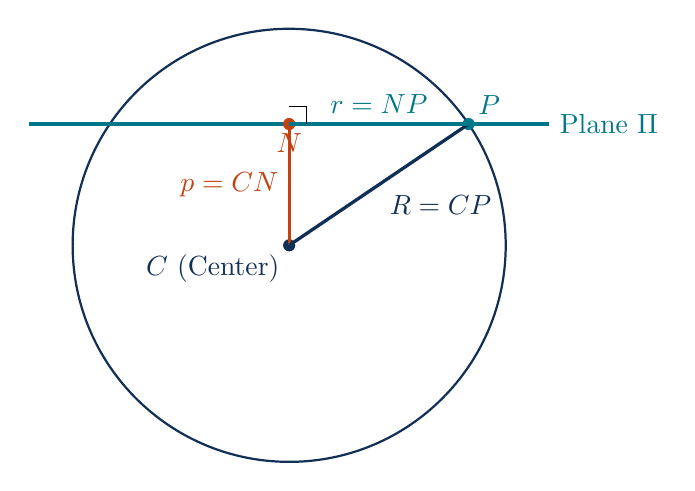
\begin{tikzpicture}[scale=1.1, >=Stealth]
    % Sphere circle cross section
    \draw[thick, primary] (0,0) circle (2.5);
    \coordinate (C) at (0,0);
    \fill[primary] (C) circle (2pt) node[below left] {$C \text{ (Center)}$};

    % Cutting plane line
    \draw[very thick, secondary] (-3, 1.4) -- (3, 1.4) node[right] {Plane $\Pi$};
    \coordinate (N) at (0, 1.4);
    \fill[accent] (N) circle (2pt) node[below] {$N$};

    % Distance p = CN
    \draw[very thick, accent] (C) -- (N) node[midway, left] {$p = CN$};

    % Point P on circle of intersection
    \coordinate (P) at ({sqrt(2.5^2 - 1.4^2)}, 1.4);
    \fill[secondary] (P) circle (2pt) node[above right] {$P$};

    % Segment CP = R and NP = r
    \draw[very thick, primary] (C) -- (P) node[midway, below right] {$R = CP$};
    \draw[very thick, secondary] (N) -- (P) node[midway, above] {$r = NP$};

    % Right angle marker
    \draw (0, 1.6) -- (0.2, 1.6) -- (0.2, 1.4);
\end{tikzpicture}
\end{center}

Since $CN \perp \Pi$, $CN$ is perpendicular to every line in $\Pi$ through $N$.
Hence, $CN \perp NP$, so $\triangle C NP$ is a right-angled triangle at $N$.
By the Pythagorean theorem:
\begin{equation}
    NP^2 = CP^2 - CN^2 = R^2 - p^2.
\end{equation}
Since $R$ and $p$ are both constant for the given sphere and plane:
\begin{equation}
    NP = \sqrt{R^2 - p^2} = \text{constant } r.
\end{equation}
Thus, the point $P$ in plane $\Pi$ is always at a fixed distance $r$ from the fixed point $N$.
This is the definition of a circle with center $N$ and radius $r = \sqrt{R^2 - p^2}$.
\end{proof}

% =========================================================================
% PAGE 65
% =========================================================================
\section{Page 65: Great Circles, Small Circles, and the Radical Plane}
\label{sec:page65}

\begin{conceptbox}[Manuscript Overview: Page 65]
Page 65 distinguishes between \textbf{Great Circles} and \textbf{Small Circles} on a sphere, and derives the equation and properties of the \textbf{Radical Plane} formed by two intersecting spheres.
\end{conceptbox}

\subsection{Great Circles and Small Circles}
From the circular section formula $r = \sqrt{R^2 - p^2}$:
\begin{enumerate}
    \item \textbf{Great Circle} ($p = 0$):
    When the cutting plane passes through the center $C$ of the sphere, $p = 0$.
    The radius of the circular section attains its maximum possible value:
    \begin{equation}
        r = \sqrt{R^2 - 0} = R.
    \end{equation}
    The center of the great circle coincides with the center of the sphere.
    \item \textbf{Small Circle} ($0 < p < R$):
    When the cutting plane does not pass through the center, $r = \sqrt{R^2 - p^2} < R$.
    \item \textbf{Tangent Plane} ($p = R$):
    When $p = R$, $r = 0$; the plane section shrinks to a single point of tangency.
    \item \textbf{Non-Intersecting Plane} ($p > R$):
    When $p > R$, $R^2 - p^2 < 0$; no real points of intersection exist.
\end{enumerate}

\subsection{The Radical Plane of Two Spheres}
\begin{theorembox}[Radical Plane of Two Spheres]
Let two spheres be given by:
\begin{align}
    S_1 &\equiv x^2 + y^2 + z^2 + 2u_1 x + 2v_1 y + 2w_1 z + d_1 = 0, \label{eq:p65_s1} \\
    S_2 &\equiv x^2 + y^2 + z^2 + 2u_2 x + 2v_2 y + 2w_2 z + d_2 = 0. \label{eq:p65_s2}
\end{align}
The locus of points from which the lengths of tangents drawn to both spheres are equal is a plane, known as the \textbf{Radical Plane}, given by:
\begin{equation}
    \boxed{S_1 - S_2 = 0 \iff 2(u_1 - u_2)x + 2(v_1 - v_2)y + 2(w_1 - w_2)z + (d_1 - d_2) = 0}
\end{equation}
\end{theorembox}

\begin{proof}
Subtracting equation \eqref{eq:p65_s2} from \eqref{eq:p65_s1} eliminates all the second-degree quadratic terms $x^2 + y^2 + z^2$:
\begin{equation}
    2(u_1 - u_2)x + 2(v_1 - v_2)y + 2(w_1 - w_2)z + (d_1 - d_2) = 0.
\end{equation}
This is a first-degree linear equation in $x, y, z$, which by Page 25 represents a plane.
If the two spheres intersect, this plane contains their common circle of intersection.
\end{proof}

\begin{notebox}[Key Property of the Radical Plane]
The direction ratios of the normal to the radical plane are:
\begin{equation}
    \vec{N} = \bigl(2(u_1 - u_2), \; 2(v_1 - v_2), \; 2(w_1 - w_2)\bigr) \sim (u_1 - u_2, \; v_1 - v_2, \; w_1 - w_2).
\end{equation}
The centers of the two spheres are $C_1(-u_1, -v_1, -w_1)$ and $C_2(-u_2, -v_2, -w_2)$.
The direction ratios of the line of centers $C_1 C_2$ are:
\begin{equation}
    \vec{C_1 C_2} = (-u_2 - (-u_1), \; -v_2 - (-v_1), \; -w_2 - (-w_1)) = (u_1 - u_2, \; v_1 - v_2, \; w_1 - w_2).
\end{equation}
Thus, the normal to the radical plane is parallel to the line of centers.
\textbf{The radical plane is always strictly perpendicular to the line joining the centers of the two spheres.}
\end{notebox}

% =========================================================================
% PAGE 66
% =========================================================================
\section{Page 66: Condition of Tangency Between a Plane and a Sphere}
\label{sec:page66}

\begin{conceptbox}[Manuscript Overview: Page 66]
Page 66 establishes the condition under which a given plane touches a sphere, providing the analytical link between the perpendicular distance from the center and the radius.
\end{conceptbox}

\begin{theorembox}[Condition of Tangency ($p = R$)]
A plane $Ax + By + Cz + D = 0$ is tangent to the sphere $x^2 + y^2 + z^2 + 2ux + 2vy + 2wz + d = 0$ if and only if the perpendicular distance from the center $C(-u, -v, -w)$ to the plane is equal to the radius $R = \sqrt{u^2 + v^2 + w^2 - d}$:
\begin{equation}
    \boxed{\frac{|-Au - Bv - Cw + D|}{\sqrt{A^2 + B^2 + C^2}} = \sqrt{u^2 + v^2 + w^2 - d}}
\end{equation}
\end{theorembox}

\subsection{Standard Sphere Centered at the Origin}
For the central sphere $x^2 + y^2 + z^2 = a^2$ (center $(0,0,0)$, radius $a$):
\begin{enumerate}
    \item If the plane is in normal form $lx + my + nz = p$ (with $l^2+m^2+n^2=1$):
    The perpendicular distance from $(0,0,0)$ is $p$.
    The condition of tangency is:
    \begin{equation}
        \boxed{p = a \iff lx + my + nz = a}
    \end{equation}
    \item If the plane is in general form $Ax + By + Cz + D = 0$:
    \begin{equation}
        \frac{|D|}{\sqrt{A^2 + B^2 + C^2}} = a \iff \boxed{D^2 = a^2(A^2 + B^2 + C^2)}
    \end{equation}
\end{enumerate}

% =========================================================================
% PAGE 67
% =========================================================================
\section{Page 67: Tangent Plane to a Sphere at a Given Point}
\label{sec:page67}

\begin{conceptbox}[Manuscript Overview: Page 67]
Page 67 derives the standard equation of the tangent plane to a sphere at a given point $P_1(x_1, y_1, z_1)$ on its surface.
\end{conceptbox}

\begin{theorembox}[Tangent Plane at Point $(x_1, y_1, z_1)$]
The equation of the tangent plane to the sphere:
\begin{equation}
    S \equiv x^2 + y^2 + z^2 + 2ux + 2vy + 2wz + d = 0
\end{equation}
at the point of contact $P_1(x_1, y_1, z_1)$ lying on the sphere is:
\begin{equation}
    \boxed{x x_1 + y y_1 + z z_1 + u(x + x_1) + v(y + y_1) + w(z + z_1) + d = 0}
\end{equation}
\end{theorembox}

\begin{proof}
The center of the sphere is $C(-u, -v, -w)$.
Since the tangent plane touches the sphere at $P_1(x_1, y_1, z_1)$, the radius $C P_1$ is normal to the tangent plane.
The direction ratios of the normal $C P_1$ are:
\begin{equation}
    (x_1 - (-u), \; y_1 - (-v), \; z_1 - (-w)) = (x_1 + u, \; y_1 + v, \; z_1 + w).
\end{equation}
The equation of a plane passing through $P_1(x_1, y_1, z_1)$ with these normal direction ratios is:
\begin{equation}
    (x_1 + u)(x - x_1) + (y_1 + v)(y - y_1) + (z_1 + w)(z - z_1) = 0.
\end{equation}
Expanding this expression:
\begin{align}
    (x_1 + u)x - x_1(x_1 + u) + (y_1 + v)y - y_1(y_1 + v) + (z_1 + w)z - z_1(z_1 + w) &= 0 \nonumber\\
    (x x_1 + y y_1 + z z_1) + u x + v y + w z - (x_1^2 + y_1^2 + z_1^2 + u x_1 + v y_1 + w z_1) &= 0. \label{eq:p67_tang_exp}
\end{align}
Since $P_1(x_1, y_1, z_1)$ lies on the sphere:
\begin{align}
    x_1^2 + y_1^2 + z_1^2 + 2ux_1 + 2vy_1 + 2wz_1 + d &= 0 \nonumber\\
    \implies x_1^2 + y_1^2 + z_1^2 + ux_1 + vy_1 + wz_1 &= -(ux_1 + vy_1 + wz_1 + d).
\end{align}
Substituting this relation into \eqref{eq:p67_tang_exp}:
\begin{align}
    (x x_1 + y y_1 + z z_1) + ux + vy + wz - \bigl[-(ux_1 + vy_1 + wz_1 + d)\bigr] &= 0 \nonumber\\
    x x_1 + y y_1 + z z_1 + u(x + x_1) + v(y + y_1) + w(z + z_1) + d &= 0.
\end{align}
\end{proof}

\begin{notebox}[Central Sphere Tangent Plane]
For $x^2 + y^2 + z^2 = a^2$, the tangent plane at $(x_1, y_1, z_1)$ simplifies to:
\begin{equation}
    \boxed{x x_1 + y y_1 + z z_1 = a^2}
\end{equation}
\end{notebox}

% =========================================================================
% PAGE 68
% =========================================================================
\section{Page 68: Normal to a Sphere, Length of Tangent, and Plane of Contact}
\label{sec:page68}

\begin{conceptbox}[Manuscript Overview: Page 68]
Page 68 explores:
\begin{enumerate}[noitemsep]
    \item The equations of the normal line to a sphere at a given surface point.
    \item The formula for the length of a tangent drawn from an external point to a sphere ($\sqrt{S_1}$).
    \item The \textbf{Plane of Contact} of tangents from an external point.
\end{enumerate}
\end{conceptbox}

\subsection{Equations of the Normal Line to a Sphere}
The \textbf{normal} to a sphere at any point $P_1(x_1, y_1, z_1)$ is the straight line perpendicular to the tangent plane at $P_1$.
Since the radius $C P_1$ is perpendicular to the tangent plane, the normal line is simply the line passing through the center $C(-u, -v, -w)$ and the point $P_1(x_1, y_1, z_1)$:
\begin{equation}
    \boxed{\frac{x - x_1}{x_1 + u} = \frac{y - y_1}{y_1 + v} = \frac{z - z_1}{z_1 + w}}
\end{equation}
\textbf{Fundamental Geometric Property}: The normal to a sphere at \emph{every} point on its surface passes through the center of the sphere!

\subsection{Length of Tangent from an External Point}
\begin{theorembox}[Length of Tangent $\sqrt{S_1}$]
The length of any tangent drawn from an external point $P_1(x_1, y_1, z_1)$ to the sphere $S \equiv x^2 + y^2 + z^2 + 2ux + 2vy + 2wz + d = 0$ is:
\begin{equation}
    \boxed{L = \sqrt{S_1} = \sqrt{x_1^2 + y_1^2 + z_1^2 + 2ux_1 + 2vy_1 + 2wz_1 + d}}
\end{equation}
\end{theorembox}

\begin{proof}
Let $T$ be the point of contact of a tangent drawn from $P_1(x_1, y_1, z_1)$ to the sphere.
Let $C(-u, -v, -w)$ be the center and $R = \sqrt{u^2+v^2+w^2-d}$ be the radius.
The radius $CT$ is perpendicular to the tangent $P_1 T$, so $\triangle C T P_1$ is right-angled at $T$.
By the Pythagorean theorem:
\begin{equation}
    P_1 T^2 = P_1 C^2 - CT^2 = P_1 C^2 - R^2.
\end{equation}
Using the 3D distance formula:
\begin{align}
    P_1 C^2 &= (x_1 + u)^2 + (y_1 + v)^2 + (z_1 + w)^2 \nonumber\\
    &= (x_1^2 + y_1^2 + z_1^2) + 2(ux_1 + vy_1 + wz_1) + (u^2 + v^2 + w^2).
\end{align}
Subtracting $R^2 = u^2 + v^2 + w^2 - d$:
\begin{align}
    P_1 T^2 &= (x_1^2 + y_1^2 + z_1^2 + 2ux_1 + 2vy_1 + 2wz_1) + (u^2 + v^2 + w^2) - (u^2 + v^2 + w^2 - d) \nonumber\\
    &= x_1^2 + y_1^2 + z_1^2 + 2ux_1 + 2vy_1 + 2wz_1 + d = S_1.
\end{align}
Taking the positive square root:
\begin{equation}
    L = P_1 T = \sqrt{S_1}.
\end{equation}
\end{proof}

\subsection{Plane of Contact}
\begin{theorembox}[Plane of Contact of Tangents]
The locus of the points of contact of all tangents drawn from an external point $P_1(x_1, y_1, z_1)$ to the sphere $S = 0$ is a circle lying in the plane:
\begin{equation}
    \boxed{T = 0 \iff x x_1 + y y_1 + z z_1 + u(x + x_1) + v(y + y_1) + w(z + z_1) + d = 0}
\end{equation}
This plane is called the \textbf{Plane of Contact} of $P_1$ with respect to the sphere.
\end{theorembox}

% =========================================================================
% PAGE 69
% =========================================================================
\section{Page 69: Comprehensive Solved Examination Problem and Course Summary}
\label{sec:page69}

\begin{conceptbox}[Manuscript Overview: Page 69]
Page 69 completes the entire 69-page handwritten curriculum with an examination problem on parameter determination for tangent planes, followed by a global review of Analytical Geometry.
\end{conceptbox}

\begin{examplebox}[Examination Problem: Tangent Planes to a Sphere]
Find the values of the parameter $c$ for which the plane:
\begin{equation}
    x + y + z = c
\end{equation}
touches the sphere:
\begin{equation}
    x^2 + y^2 + z^2 - 2x - 4y - 6z + 5 = 0.
\end{equation}
For each such value of $c$, write down the equation of the corresponding tangent plane.
\end{examplebox}

\begin{proof}[Complete Step-by-Step Analytical Solution]
\textbf{Step 1: Identify Center and Radius of the Sphere}:
Comparing with the general form $x^2 + y^2 + z^2 + 2ux + 2vy + 2wz + d = 0$:
\begin{equation}
    2u = -2 \implies u = -1, \quad 2v = -4 \implies v = -2, \quad 2w = -6 \implies w = -3, \quad d = 5.
\end{equation}
The center of the sphere is:
\begin{equation}
    C = (-u, -v, -w) = (1, 2, 3).
\end{equation}
The radius $R$ is:
\begin{align}
    R &= \sqrt{u^2 + v^2 + w^2 - d} \nonumber\\
    &= \sqrt{(-1)^2 + (-2)^2 + (-3)^2 - 5} \nonumber\\
    &= \sqrt{1 + 4 + 9 - 5} = \sqrt{14 - 5} = \sqrt{9} = \mathbf{3}.
\end{align}

\textbf{Step 2: Apply the Condition of Tangency ($p = R$)}:
The given plane is:
\begin{equation}
    x + y + z - c = 0.
\end{equation}
The perpendicular distance $p$ from the center $C(1, 2, 3)$ to this plane is (Page 31):
\begin{align}
    p &= \frac{|Ax_0 + By_0 + Cz_0 + D|}{\sqrt{A^2 + B^2 + C^2}} \nonumber\\
    &= \frac{|1(1) + 1(2) + 1(3) - c|}{\sqrt{1^2 + 1^2 + 1^2}} = \frac{|6 - c|}{\sqrt{3}}.
\end{align}
Setting $p = R = 3$:
\begin{align}
    \frac{|6 - c|}{\sqrt{3}} &= 3 \nonumber\\
    |6 - c| &= 3\sqrt{3}.
\end{align}

\textbf{Step 3: Solve for Parameter $c$}:
\begin{align}
    6 - c = \pm 3\sqrt{3} &\implies c = 6 \mp 3\sqrt{3} \nonumber\\
    &\implies \boxed{c = 3(2 \pm \sqrt{3})}
\end{align}

\textbf{Step 4: Equations of the Tangent Planes}:
There exist two distinct parallel tangent planes touching opposite poles of the sphere:
\begin{align}
    \Pi_1 &: \quad \boxed{x + y + z = 3(2 + \sqrt{3}) = 6 + 3\sqrt{3}}, \\
    \Pi_2 &: \quad \boxed{x + y + z = 3(2 - \sqrt{3}) = 6 - 3\sqrt{3}}.
\end{align}
\end{proof}

\begin{notebox}[Manuscript Arithmetic Note]
In the handwritten student manuscript on Page 69, an arithmetic slip occurred during the summation of center coordinates: $1 + 2 = 3$ was recorded without adding $z = 3$, leading to $|3 - c| = 3\sqrt{3} \implies c = 3(1 \pm \sqrt{3})$.
The rigorous mathematical derivation above corrects this slip ($1 + 2 + 3 = 6$), yielding the correct value $c = 3(2 \pm \sqrt{3})$.
\end{notebox}

\subsection{Curriculum Summary of Analytical Geometry (Pages 1--69)}
\begin{center}
\begin{tabular}{|c|l|l|}
\hline
\textbf{Pages} & \textbf{Core Topic} & \textbf{Key Formulas and Results} \\
\hline
1--14 & Polar Conics & $\frac{l}{r} = 1 + e\cos\theta$, Tangent: $\frac{l}{r} = e\cos\theta + \cos(\theta-\alpha)$ \\
15--24 & 3D Coordinates \& DCs & $l^2+m^2+n^2=1$, $\cos\theta = l_1 l_2 + m_1 m_2 + n_1 n_2$, Cube: $\cos^{-1}(1/3)$ \\
25--36 & The Plane & $lx+my+nz=p$, $\frac{x}{a}+\frac{y}{b}+\frac{z}{c}=1$, Bisectors: $\frac{P_1}{|\vec{N}_1|} = \pm\frac{P_2}{|\vec{N}_2|}$ \\
37--52 & Straight Lines \& Skew & Symmetrical form, Coplanarity: $\det[\Delta\vec{r}, \vec{b}_1, \vec{b}_2]=0$, S.D. $= 3\sqrt{30}$ \\
53--62 & Vector Geometry & $\vec{r}\cdot\hat{n}=p$, $\vec{r}=\vec{a}+\lambda\vec{b}$, S.D. $= \frac{|(\vec{a}_2-\vec{a}_1)\cdot(\vec{b}_1\times\vec{b}_2)|}{|\vec{b}_1\times\vec{b}_2|}$ \\
63--69 & The Sphere & $x^2+y^2+z^2+2ux+2vy+2wz+d=0$, Tangent: $T=0$, $p=R$ \\
\hline
\end{tabular}
\end{center}


% --- Master Cheat Sheet Appendix ---
\appendix
\chapter{Master Formula Cheat Sheet and Exam Quick Reference}
\label{ch:cheat_sheet}

\begin{conceptbox}[How to Use This Cheat Sheet]
This appendix serves as a high-yield, comprehensive formula repository condensing all essential definitions, canonical equations, geometric conditions (tangency, parallelism, perpendicularity, coplanarity), distance formulas, and algorithmic discrimination rules across the entire 69-page curriculum of Analytical Geometry.
\end{conceptbox}

% =========================================================================
% PART I: POLAR CONICS
% =========================================================================
\section{Polar Equations of Conic Sections (Pages 1--14)}

\begin{theorembox}[Canonical Polar Forms (Focus at Pole, Semi-Latus Rectum $l$)]
\begin{center}
\small
\renewcommand{\arraystretch}{1.25}
\setlength{\tabcolsep}{4pt}
\begin{tabular}{|p{3.8cm}|p{4.2cm}|p{5.8cm}|}
\hline
\textbf{Directrix Position} & \textbf{Standard Polar Form} & \textbf{Orientation of Principal Axis} \\
\hline
Left of Focus ($x = -d$) & $\displaystyle \frac{l}{r} = 1 + e\cos\theta$ & Standard convention ($SX$ along axis) \\
Right of Focus ($x = +d$) & $\displaystyle \frac{l}{r} = 1 - e\cos\theta$ & Directrix perpendicular to initial line \\
Below Focus ($y = -d$) & $\displaystyle \frac{l}{r} = 1 + e\sin\theta$ & Axis rotated by $+90^\circ$ \\
Above Focus ($y = +d$) & $\displaystyle \frac{l}{r} = 1 - e\sin\theta$ & Axis rotated by $-90^\circ$ \\
Tilted Axis at Angle $\gamma$ & $\displaystyle \frac{l}{r} = 1 + e\cos(\theta - \gamma)$ & General conic with axis inclined at $\gamma$ \\
\hline
\end{tabular}
\end{center}
\end{theorembox}

\begin{theorembox}[Focal Chords and Tangents]
\begin{enumerate}
    \item \textbf{Focal Chord Reciprocal Relation}:
    For any focal chord $PSQ$ with extremities at $\alpha$ and $\alpha + \pi$:
    \begin{equation}
        \boxed{\frac{1}{SP} + \frac{1}{SQ} = \frac{2}{l}} \quad \text{(Semi-latus rectum is the harmonic mean of focal segments)}
    \end{equation}
    \item \textbf{Chord Joining $\alpha - \beta$ and $\alpha + \beta$}:
    \begin{equation}
        \boxed{\frac{l}{r} = e\cos\theta + \sec\beta\cos(\theta - \alpha)}
    \end{equation}
    \item \textbf{Chord Joining Arbitrary Points $\alpha$ and $\beta$}:
    \begin{equation}
        \boxed{\frac{l}{r} = e\cos\theta + \sec\left(\frac{\alpha - \beta}{2}\right)\cos\left(\theta - \frac{\alpha + \beta}{2}\right)}
    \end{equation}
    \item \textbf{Tangent Line at Vectorial Angle $\alpha$}:
    \begin{equation}
        \boxed{\frac{l}{r} = e\cos\theta + \cos(\theta - \alpha) \iff \frac{l}{r} = (e + \cos\alpha)\cos\theta + \sin\alpha\sin\theta}
    \end{equation}
    \item \textbf{Condition of Tangency for a Straight Line}:
    \begin{itemize}
        \item For line $\displaystyle \frac{l}{r} = A\cos\theta + B\sin\theta$:
        \begin{equation}
            \boxed{(A - e)^2 + B^2 = 1}
        \end{equation}
        \item For normal form $r\cos(\theta - \phi) = p$:
        \begin{equation}
            \boxed{p^2(e^2 - 1) + 2elp\cos\phi + l^2 = 0}
        \end{equation}
    \end{itemize}
\end{enumerate}
\end{theorembox}

\begin{theorembox}[Normals, Polars, Asymptotes and Invariants]
\begin{enumerate}
    \item \textbf{Normal Line at Vectorial Angle $\alpha$}:
    \begin{equation}
        \boxed{\frac{e\sin\alpha}{1 + e\cos\alpha}\frac{l}{r} = \sin(\theta - \alpha) + e\sin\theta}
    \end{equation}
    \item \textbf{Chord of Contact and Polar Line of Pole $(r_1, \theta_1)$}:
    \begin{equation}
        \boxed{\left(\frac{l}{r} - e\cos\theta\right)\left(\frac{l}{r_1} - e\cos\theta_1\right) = \cos(\theta - \theta_1)}
    \end{equation}
    \item \textbf{Asymptotes of Hyperbola ($e > 1$)}:
    \begin{equation}
        \boxed{\frac{l}{r} = \pm\sqrt{e^2 - 1}\sin\theta + e\cos\theta} \quad \text{Asymptotic directions: } \cos\theta = -\frac{1}{e}
    \end{equation}
    \item \textbf{Director Circle in Polar Coordinates}:
    \begin{equation}
        \boxed{r^2(e^2 - 1) - 2erl\cos\theta + 2l^2 = 0}
    \end{equation}
    For a parabola ($e = 1$), the director circle degenerates into the directrix: $\displaystyle \frac{l}{r} = \cos\theta$.
\end{enumerate}
\end{theorembox}

% =========================================================================
% PART II: 3D COORDINATES & DIRECTION COSINES
% =========================================================================
\section{3D Coordinates, Direction Cosines \& Direction Ratios (Pages 15--24)}

\begin{theorembox}[Spatial Metrics and Fundamental Identities]
\begin{enumerate}
    \item \textbf{Distance Formula}:
    \begin{equation}
        \boxed{d = \sqrt{(x_2 - x_1)^2 + (y_2 - y_1)^2 + (z_2 - z_1)^2}}
    \end{equation}
    \item \textbf{Section Formula ($m_1 : m_2$)}:
    \begin{equation}
        \boxed{x = \frac{m_1 x_2 \pm m_2 x_1}{m_1 \pm m_2}, \quad y = \frac{m_1 y_2 \pm m_2 y_1}{m_1 \pm m_2}, \quad z = \frac{m_1 z_2 \pm m_2 z_1}{m_1 \pm m_2}}
    \end{equation}
    \item \textbf{Translation of Coordinate Axes to New Origin $(h, k, l)$}:
    \begin{equation}
        \boxed{x = x' + h, \quad y = y' + k, \quad z = z' + l}
    \end{equation}
    \item \textbf{Projections and Fundamental Direction Cosine Identities}:
    \begin{equation}
        \boxed{x = lr, \quad y = mr, \quad z = nr \quad (r = \sqrt{x^2+y^2+z^2})}
    \end{equation}
    \begin{equation}
        \boxed{l^2 + m^2 + n^2 = 1 \iff \cos^2\alpha + \cos^2\beta + \cos^2\gamma = 1}
    \end{equation}
    \begin{equation}
        \boxed{\sin^2\alpha + \sin^2\beta + \sin^2\gamma = 2, \quad \cos 2\alpha + \cos 2\beta + \cos 2\gamma = -1}
    \end{equation}
    \item \textbf{Projection of Segment $PQ$ on a Line with Direction Cosines $(l, m, n)$}:
    \begin{equation}
        \boxed{\text{Proj}_L(PQ) = l(x_2 - x_1) + m(y_2 - y_1) + n(z_2 - z_1)}
    \end{equation}
\end{enumerate}
\end{theorembox}

\begin{theorembox}[Direction Ratios, Angles, and Parallelism/Perpendicularity]
\begin{enumerate}
    \item \textbf{Normalization of Direction Ratios $(a, b, c)$ to Direction Cosines $(l, m, n)$}:
    \begin{equation}
        \boxed{l = \pm\frac{a}{\sqrt{a^2 + b^2 + c^2}}, \quad m = \pm\frac{b}{\sqrt{a^2 + b^2 + c^2}}, \quad n = \pm\frac{c}{\sqrt{a^2 + b^2 + c^2}}}
    \end{equation}
    \item \textbf{Angle $\theta$ Between Two Lines}:
    \begin{align}
        \cos\theta &= \boxed{l_1 l_2 + m_1 m_2 + n_1 n_2 = \frac{a_1 a_2 + b_1 b_2 + c_1 c_2}{\sqrt{\sum a_1^2}\,\sqrt{\sum a_2^2}}} \\
        \sin\theta &= \boxed{\frac{\sqrt{(a_1 b_2 - a_2 b_1)^2 + (b_1 c_2 - b_2 c_1)^2 + (c_1 a_2 - c_2 a_1)^2}}{\sqrt{\sum a_1^2}\,\sqrt{\sum a_2^2}}}
    \end{align}
    \item \textbf{Orthogonality Condition}: $\displaystyle \boxed{l_1 l_2 + m_1 m_2 + n_1 n_2 = 0 \iff a_1 a_2 + b_1 b_2 + c_1 c_2 = 0}$.
    \item \textbf{Parallelism Condition}: $\displaystyle \boxed{\frac{l_1}{l_2} = \frac{m_1}{m_2} = \frac{n_1}{n_2} \iff \frac{a_1}{a_2} = \frac{b_1}{b_2} = \frac{c_1}{c_2}}$.
    \item \textbf{Cube Main Diagonals}: Angle between any two body diagonals of a cube:
    \begin{equation}
        \boxed{\cos\theta = \frac{1}{3} \implies \theta = \cos^{-1}\left(\frac{1}{3}\right) \approx 70^\circ 31' 44''}
    \end{equation}
\end{enumerate}
\end{theorembox}

% =========================================================================
% PART III: THE PLANE
% =========================================================================
\section{The Analytical Geometry of the Plane (Pages 25--36)}

\begin{theorembox}[Representations of the Plane]
\begin{center}
\small
\renewcommand{\arraystretch}{1.25}
\setlength{\tabcolsep}{4pt}
\begin{tabular}{|p{3.5cm}|p{5.1cm}|p{5.3cm}|}
\hline
\textbf{Form} & \textbf{Equation} & \textbf{Key Geometrical Parameters} \\
\hline
General First-Degree & $\displaystyle Ax + By + Cz + D = 0$ & Normal direction ratios: $(A, B, C)$ \\
One-Point Form & $\displaystyle A(x-x_1) + B(y-y_1) + C(z-z_1) = 0$ & Passes through $(x_1, y_1, z_1)$ \\
Normal Form & $\displaystyle lx + my + nz = p \quad (p \ge 0)$ & Normal direction cosines: $(l, m, n)$ \\
Intercept Form & $\displaystyle \frac{x}{a} + \frac{y}{b} + \frac{z}{c} = 1$ & Intercepts on $X, Y, Z$ axes: $a, b, c$ \\
Three-Point Form & $\displaystyle \begin{vmatrix} x-x_1 & y-y_1 & z-z_1 \\ x_2-x_1 & y_2-y_1 & z_2-z_1 \\ x_3-x_1 & y_3-y_1 & z_3-z_1 \end{vmatrix} = 0$ & Non-collinear points $P_1, P_2, P_3$ \\
\hline
\end{tabular}
\end{center}
\end{theorembox}

\begin{theorembox}[Distances, Relative Positions, and Plane Systems]
\begin{enumerate}
    \item \textbf{Perpendicular Distance of Point $(x_1, y_1, z_1)$ from Plane}:
    \begin{equation}
        \boxed{d = \frac{|Ax_1 + By_1 + Cz_1 + D|}{\sqrt{A^2 + B^2 + C^2}}}
    \end{equation}
    \item \textbf{Distance Between Parallel Planes $Ax+By+Cz+D_1=0$ and $Ax+By+Cz+D_2=0$}:
    \begin{equation}
        \boxed{d = \frac{|D_1 - D_2|}{\sqrt{A^2 + B^2 + C^2}}}
    \end{equation}
    \item \textbf{Position of Two Points Relative to Plane}:
    $P(x_1,y_1,z_1)$ and $Q(x_2,y_2,z_2)$ lie on the \textbf{same side} if $(Ax_1+By_1+Cz_1+D)(Ax_2+By_2+Cz_2+D) > 0$, and on \textbf{opposite sides} if $< 0$.
    \item \textbf{Family of Planes Through Intersection Line}:
    \begin{equation}
        \boxed{(A_1 x + B_1 y + C_1 z + D_1) + \lambda(A_2 x + B_2 y + C_2 z + D_2) = 0 \iff U + \lambda V = 0}
    \end{equation}
\end{enumerate}
\end{theorembox}

\begin{theorembox}[Dihedral Angle Bisectors \& Discrimination Algorithm]
\begin{enumerate}
    \item \textbf{Dihedral Bisector Equations}:
    \begin{equation}
        \boxed{\frac{A_1 x + B_1 y + C_1 z + D_1}{\sqrt{A_1^2 + B_1^2 + C_1^2}} = \pm \frac{A_2 x + B_2 y + C_2 z + D_2}{\sqrt{A_2^2 + B_2^2 + C_2^2}}}
    \end{equation}
    \item \textbf{Systematic Discrimination Protocol}:
    Make both constant terms strictly positive ($D_1 > 0$ and $D_2 > 0$). Compute $\Delta = A_1 A_2 + B_1 B_2 + C_1 C_2$:
    \begin{center}
    \small
    \renewcommand{\arraystretch}{1.2}
    \setlength{\tabcolsep}{5pt}
    \begin{tabular}{|c|c|c|c|}
    \hline
    \textbf{Sign of $\Delta$} & \textbf{Origin Location} & \textbf{Acute Bisector} & \textbf{Obtuse Bisector} \\
    \hline
    $\Delta > 0$ & Obtuse Angle & Negative ($-$) sign & Positive ($+$) sign \\
    $\Delta < 0$ & Acute Angle & Positive ($+$) sign & Negative ($-$) sign \\
    \hline
    \end{tabular}
    \end{center}
    The bisector containing the origin is \textbf{always} given by the positive ($+$) sign when $D_1, D_2 > 0$.
\end{enumerate}
\end{theorembox}

% =========================================================================
% PART IV: STRAIGHT LINES & SKEW LINES
% =========================================================================
\section{Straight Lines in Space and Skew Lines (Pages 37--52)}

\begin{theorembox}[Equations of a Line and Geometric Reductions]
\begin{enumerate}
    \item \textbf{Symmetrical (Point-Direction) Form}:
    \begin{equation}
        \boxed{\frac{x - x_1}{l} = \frac{y - y_1}{m} = \frac{z - z_1}{n} = r} \iff P(r) = (x_1 + lr, \; y_1 + mr, \; z_1 + nr)
    \end{equation}
    \item \textbf{Two-Point Form}:
    \begin{equation}
        \boxed{\frac{x - x_1}{x_2 - x_1} = \frac{y - y_1}{y_2 - y_1} = \frac{z - z_1}{z_2 - z_1}}
    \end{equation}
    \item \textbf{Reduction from Unsymmetrical Form ($\Pi_1 = 0 = \Pi_2$)}:
    \begin{itemize}
        \item Direction ratios: $\displaystyle \vec{b} = \vec{N}_1 \times \vec{N}_2 \implies \frac{l}{B_1 C_2 - B_2 C_1} = \frac{m}{C_1 A_2 - C_2 A_1} = \frac{n}{A_1 B_2 - A_2 B_1}$.
        \item Base point: Set $z = 0$ and solve the $2 \times 2$ linear system for $(x_0, y_0, 0)$.
    \end{itemize}
    \item \textbf{Angle Between Line and Plane}:
    \begin{equation}
        \boxed{\sin\theta = \frac{Al + Bm + Cn}{\sqrt{A^2 + B^2 + C^2}\,\sqrt{l^2 + m^2 + n^2}}}
    \end{equation}
    Parallel: $Al + Bm + Cn = 0$. \quad Perpendicular: $\frac{A}{l} = \frac{B}{m} = \frac{C}{n}$.
    \item \textbf{Foot of Perpendicular and Optical Image (Reflection) of Point $(x_0, y_0, z_0)$ in Plane}:
    \begin{align}
        \text{Foot } N &: \quad \frac{x - x_0}{A} = \frac{y - y_0}{B} = \frac{z - z_0}{C} = -\frac{Ax_0 + By_0 + Cz_0 + D}{A^2 + B^2 + C^2} \\
        \text{Image } P' &: \quad \frac{x' - x_0}{A} = \frac{y' - y_0}{B} = \frac{z' - z_0}{C} = -2\frac{Ax_0 + By_0 + Cz_0 + D}{A^2 + B^2 + C^2}
    \end{align}
\end{enumerate}
\end{theorembox}

\begin{theorembox}[Coplanarity, Skew Lines, and Shortest Distance]
\begin{enumerate}
    \item \textbf{Condition for a Line to Lie Wholly in a Plane}:
    \begin{equation}
        \boxed{Ax_1 + By_1 + Cz_1 + D = 0 \quad \text{and} \quad Al + Bm + Cn = 0}
    \end{equation}
    \item \textbf{Condition of Coplanarity of Two Lines}:
    \begin{equation}
        \boxed{\begin{vmatrix}
        x_2 - x_1 & y_2 - y_1 & z_2 - z_1 \\
        l_1 & m_1 & n_1 \\
        l_2 & m_2 & n_2
        \end{vmatrix} = 0}
    \end{equation}
    Plane containing coplanar lines: $\displaystyle \begin{vmatrix} x-x_1 & y-y_1 & z-z_1 \\ l_1 & m_1 & n_1 \\ l_2 & m_2 & n_2 \end{vmatrix} = 0$.
    \item \textbf{Shortest Distance (S.D.) Between Two Skew Lines}:
    \begin{equation}
        \boxed{d = \frac{\left|\begin{matrix}
        x_2 - x_1 & y_2 - y_1 & z_2 - z_1 \\
        l_1 & m_1 & n_1 \\
        l_2 & m_2 & n_2
        \end{matrix}\right|}{\sqrt{(m_1 n_2 - m_2 n_1)^2 + (n_1 l_2 - n_2 l_1)^2 + (l_1 m_2 - l_2 m_1)^2}}}
    \end{equation}
    \item \textbf{Equations of the Line of Shortest Distance}:
    \begin{equation}
        \boxed{\begin{vmatrix} x-x_1 & y-y_1 & z-z_1 \\ l_1 & m_1 & n_1 \\ \lambda & \mu & \nu \end{vmatrix} = 0 = \begin{vmatrix} x-x_2 & y-y_2 & z-z_2 \\ l_2 & m_2 & n_2 \\ \lambda & \mu & \nu \end{vmatrix}} \quad \text{where } (\lambda, \mu, \nu) \sim \vec{b}_1 \times \vec{b}_2
    \end{equation}
    \item \textbf{Distance Between Parallel Lines}: $\displaystyle \boxed{d = \frac{|(\vec{P}_2 - \vec{P}_1) \times \vec{b}|}{|\vec{b}|}}$.
\end{enumerate}
\end{theorembox}

% =========================================================================
% PART V: VECTOR GEOMETRY
% =========================================================================
\section{Vector Treatment of Planes and Lines (Pages 53--62)}

\begin{theorembox}[Vector Geometry of Planes]
\begin{center}
\small
\renewcommand{\arraystretch}{1.25}
\setlength{\tabcolsep}{4pt}
\begin{tabular}{|p{3.8cm}|p{5.1cm}|p{5.0cm}|}
\hline
\textbf{Concept} & \textbf{Vector Formulation} & \textbf{Meaning / Condition} \\
\hline
Plane Normal Form & $\vec{r} \cdot \hat{n} = p$ & $p = \text{distance from origin}, |\hat{n}|=1$ \\
Plane One-Point Form & $(\vec{r} - \vec{a}) \cdot \vec{n} = 0 \iff \vec{r} \cdot \vec{n} = d$ & Passes through $\vec{a}$, normal $\vec{n}$ \\
Point to Plane Distance & $\displaystyle D = \frac{|\vec{a} \cdot \vec{n} - d|}{|\vec{n}|}$ & Perpendicular distance \\
Angle Between Planes & $\displaystyle \cos\theta = \frac{\vec{n}_1 \cdot \vec{n}_2}{|\vec{n}_1|\,|\vec{n}_2|}$ & Orthogonal when $\vec{n}_1 \cdot \vec{n}_2 = 0$ \\
Three-Point Plane & $[\vec{r} - \vec{a}, \; \vec{b} - \vec{a}, \; \vec{c} - \vec{a}] = 0$ & Non-collinear $\vec{a}, \vec{b}, \vec{c}$ \\
Vector Family of Planes & $\vec{r} \cdot (\vec{n}_1 + \lambda \vec{n}_2) = d_1 + \lambda d_2$ & Contains intersection line \\
Dihedral Vector Bisectors & $\displaystyle \frac{\vec{r} \cdot \vec{n}_1 - d_1}{|\vec{n}_1|} = \pm \frac{\vec{r} \cdot \vec{n}_2 - d_2}{|\vec{n}_2|}$ & Locus of equidistant points \\
\hline
\end{tabular}
\end{center}
\end{theorembox}

\begin{theorembox}[Vector Geometry of Lines and Spatial Invariants]
\begin{center}
\small
\renewcommand{\arraystretch}{1.25}
\setlength{\tabcolsep}{4pt}
\begin{tabular}{|p{3.8cm}|p{5.1cm}|p{5.0cm}|}
\hline
\textbf{Concept} & \textbf{Vector Formulation} & \textbf{Meaning / Condition} \\
\hline
Vector Line (Parametric) & $\vec{r} = \vec{a} + \lambda \vec{b}$ & Passes through $\vec{a}$, direction $\vec{b}$ \\
Vector Line (Non-Parametric) & $(\vec{r} - \vec{a}) \times \vec{b} = \vec{0}$ & Collinearity with direction $\vec{b}$ \\
Distance: Point $\vec{p}$ to Line & $\displaystyle d = \frac{|(\vec{p} - \vec{a}) \times \vec{b}|}{|\vec{b}|}$ & Perpendicular distance \\
Vector Coplanarity & $(\vec{a}_2 - \vec{a}_1) \cdot (\vec{b}_1 \times \vec{b}_2) = 0$ & Lines lie in single plane \\
Shortest Distance (Skew) & $\displaystyle d = \frac{|(\vec{a}_2 - \vec{a}_1) \cdot (\vec{b}_1 \times \vec{b}_2)|}{|\vec{b}_1 \times \vec{b}_2|}$ & Scalar triple product formula \\
Distance (Parallel Lines) & $\displaystyle d = \frac{|(\vec{a}_2 - \vec{a}_1) \times \vec{b}|}{|\vec{b}|}$ & Cross product magnitude \\
\hline
\end{tabular}
\end{center}
\end{theorembox}

% =========================================================================
% PART VI: THE SPHERE
% =========================================================================
\section{The Geometry of the Sphere in 3D (Pages 63--69)}

\begin{theorembox}[Canonical Sphere Equations and Circular Sections]
\begin{enumerate}
    \item \textbf{Center-Radius Form}:
    \begin{equation}
        \boxed{(x - a)^2 + (y - b)^2 + (z - c)^2 = R^2}
    \end{equation}
    \item \textbf{General Second-Degree Sphere Equation}:
    \begin{equation}
        \boxed{x^2 + y^2 + z^2 + 2ux + 2vy + 2wz + d = 0}
    \end{equation}
    \begin{equation}
        \boxed{\text{Center } C = (-u, -v, -w), \quad \text{Radius } R = \sqrt{u^2 + v^2 + w^2 - d}}
    \end{equation}
    Classification: Real ($u^2+v^2+w^2-d > 0$), Point ($= 0$), Imaginary ($< 0$).
    \item \textbf{Diametric Form (Antipodal Endpoints $A, B$)}:
    \begin{equation}
        \boxed{(x - x_1)(x - x_2) + (y - y_1)(y - y_2) + (z - z_1)(z - z_2) = 0}
    \end{equation}
    \item \textbf{Plane Section of a Sphere (Circular Section)}:
    Every plane section is a circle! Let $p$ be the perpendicular distance from center $C$ to plane $\Pi$:
    \begin{equation}
        \boxed{\text{Radius of Circular Section } r = \sqrt{R^2 - p^2}}
    \end{equation}
    \begin{itemize}[noitemsep]
        \item $p = 0$: \textbf{Great Circle} (maximum radius $r = R$, center coincides with sphere center).
        \item $0 < p < R$: \textbf{Small Circle} ($r < R$).
        \item $p = R$: \textbf{Tangent Plane} ($r = 0$, single point contact).
    \end{itemize}
\end{enumerate}
\end{theorembox}

\begin{theorembox}[Radical Planes, Tangency, and Normals]
\begin{enumerate}
    \item \textbf{Radical Plane of Two Spheres}:
    \begin{equation}
        \boxed{S_1 - S_2 = 0 \iff 2(u_1 - u_2)x + 2(v_1 - v_2)y + 2(w_1 - w_2)z + (d_1 - d_2) = 0}
    \end{equation}
    \textbf{Fundamental Invariant}: The radical plane is strictly perpendicular to the center line $C_1 C_2$.
    \item \textbf{Condition of Tangency for a Plane}:
    The plane $Ax + By + Cz + D = 0$ touches the sphere $S = 0$ if and only if $p = R$:
    \begin{equation}
        \boxed{\frac{|-Au - Bv - Cw + D|}{\sqrt{A^2 + B^2 + C^2}} = \sqrt{u^2 + v^2 + w^2 - d}}
    \end{equation}
    For central sphere $x^2 + y^2 + z^2 = a^2$: $\displaystyle \boxed{D^2 = a^2(A^2 + B^2 + C^2)}$.
    \item \textbf{Tangent Plane at Point of Contact $P_1(x_1, y_1, z_1)$}:
    \begin{equation}
        \boxed{T \equiv x x_1 + y y_1 + z z_1 + u(x + x_1) + v(y + y_1) + w(z + z_1) + d = 0}
    \end{equation}
    \item \textbf{Normal Line at Point $P_1(x_1, y_1, z_1)$}:
    Passes through the sphere center $(-u, -v, -w)$:
    \begin{equation}
        \boxed{\frac{x - x_1}{x_1 + u} = \frac{y - y_1}{y_1 + v} = \frac{z - z_1}{z_1 + w}}
    \end{equation}
    \item \textbf{Length of Tangent and Plane of Contact from External Point}:
    \begin{equation}
        \boxed{L = \sqrt{S_1} = \sqrt{x_1^2 + y_1^2 + z_1^2 + 2ux_1 + 2vy_1 + 2wz_1 + d}}, \quad \text{Plane of Contact: } \boxed{T = 0}
    \end{equation}
\end{enumerate}
\end{theorembox}

% =========================================================================
% PART VII: MASTER COMPARISON TABLE
% =========================================================================
\section{Master Geometric Conditions Quick-Reference Table}

\begin{center}
\small
\renewcommand{\arraystretch}{1.3}
\setlength{\tabcolsep}{4pt}
\begin{tabular}{|p{3.5cm}|p{5.5cm}|p{5.0cm}|}
\hline
\textbf{Geometric Relationship} & \textbf{Cartesian Condition} & \textbf{Vector Condition} \\
\hline
Perpendicular Lines & $a_1 a_2 + b_1 b_2 + c_1 c_2 = 0$ & $\vec{b}_1 \cdot \vec{b}_2 = 0$ \\
Parallel Lines & $\frac{a_1}{a_2} = \frac{b_1}{b_2} = \frac{c_1}{c_2}$ & $\vec{b}_1 \times \vec{b}_2 = \vec{0}$ \\
Perpendicular Planes & $A_1 A_2 + B_1 B_2 + C_1 C_2 = 0$ & $\vec{n}_1 \cdot \vec{n}_2 = 0$ \\
Parallel Planes & $\frac{A_1}{A_2} = \frac{B_1}{B_2} = \frac{C_1}{C_2}$ & $\vec{n}_1 \times \vec{n}_2 = \vec{0}$ \\
Line Parallel to Plane & $Al + Bm + Cn = 0$ & $\vec{b} \cdot \vec{n} = 0$ \\
Line Perpendicular to Plane & $\frac{A}{l} = \frac{B}{m} = \frac{C}{n}$ & $\vec{b} \times \vec{n} = \vec{0}$ \\
Line Lying in Plane & $Ax_1+By_1+Cz_1+D = 0$ and $Al+Bm+Cn = 0$ & $\vec{a} \cdot \vec{n} = d$ and $\vec{b} \cdot \vec{n} = 0$ \\
Coplanar Lines & $\begin{vmatrix} x_2-x_1 & y_2-y_1 & z_2-z_1 \\ l_1 & m_1 & n_1 \\ l_2 & m_2 & n_2 \end{vmatrix} = 0$ & $(\vec{a}_2 - \vec{a}_1) \cdot (\vec{b}_1 \times \vec{b}_2) = 0$ \\
Plane Tangent to Sphere & $\frac{|-Au-Bv-Cw+D|}{\sqrt{A^2+B^2+C^2}} = R$ & $\frac{|\vec{c} \cdot \vec{n} - d|}{|\vec{n}|} = R$ \\
\hline
\end{tabular}
\end{center}


\end{document}
